\newcommand{\mypapersize}{A4}
%% e.g., "A4", "letter", "legal", "executive", ...
%% The size of the paper of the resulting PDF file.

\newcommand{\mylaterality}{oneside}
%% "oneside" or "twoside"
%% Either you are creating a document which is printed on both, left pages
%% and right pages (twoside) or you create a document which is printed
%% on right pages only (oneside).

\newcommand{\mydraft}{false}
%% "true" or "false"
%% Use draft mode? If true, included graphics are replaced by empty
%% rectangles (of same size) and overfull boxes (in margin space) are
%% marked with black box (-> easy to spot!)

\newcommand{\myparskip}{half}
\setlength{\parindent}{2em}
%% e.g., "no", "full", "half", ...
%% How to separate paragraphs: indention ("no") or spacing ("half",
%% "full", ...).

\newcommand{\myBCOR}{0mm}
%% Inner binding correction. This value depends on the method which is
%% being used to bind your printed result. Some techniques do not
%% require a binding correction at all ("0mm"), other require for
%% example "5mm". Refer to KOMA script documentation for a detailed
%% explanation what a binding correction is and how to measure it.

\newcommand{\myfontsize}{12pt}
%% e.g., 10pt, 11pt, 12pt
%% The font size of the main text in pt (points).

\newcommand{\mylinespread}{1.0}
%% e.g., 1.0, 1.5, 2.0
%% Line spacing in %/100. For example 1.5 means 150% of the usual line
%% spacing. Please use with caution: 100% ("1.0") is fine because the
%% font was designed for it.

\newcommand{\mylanguage}{american}
%% "english,ngerman", "ngerman,english", ...
%% NOTE: The *last* language is the active one!
%% See babel documentation for further details.

%% BibLaTeX-settings: (see biblatex reference for further description)
\newcommand{\mybiblatexstyle}{ieee}
%% e.g., "alphabetic", "authoryear", ...
%% The biblatex style which is being used for referencing. See
%% biblatex documentation for further details and more values.
%%
%% CAUTION: if you change the style, please check for (in)compatible
%%          "biblatex" package options in the file
%%          "template/preamble.tex"! For example: "alphabetic" does
%%          not have an option "dashed=..." and causes an error if it
%%          does not get removed from the list of options.

\newcommand{\mybiblatexdashed}{false}  %% "true" or "false"
%% If true: replace recurring reference authors with a dash.

\newcommand{\mybiblatexbackref}{true}  %% "true" or "false"
%% If true: create backward links from reference to citations.

\newcommand{\mybiblatexfile}{references-biblatex.bib}
%% Name of the biblatex file that holds the references.

\newcommand{\mydispositioncolor}{0,0,0}
%% e.g., "30,103,182" (blue/turquois), "0,0,0" (black), ...
%% Color of the headings and so forth in RGB (red,green,blue) values.
%% NOTE: if you are using "0,0,0" for black, printers might still
%%       recognize pages as color pages. In case this is a problem
%%       (paying for color print-outs vs. paying for b/w-printouts)
%%       please edit file "template/preamble.tex" and change
%%       "\definecolor{DispositionColor}{RGB}{\mydispositioncolor}"
%%       to "\definecolor{DispositionColor}{gray}{0}" and thus
%%       overwriting the value of \mydispositioncolor above.

\newcommand{\mycolorlinks}{true}  %% "true" or "false"
%% Enables or disables colored links (hyperref package).

\newcommand{\mytitlepage}{template/title_Thesis_TU_Graz}

%% Your own or one of following pre-defined title pages:
%% "template/title_plain_maketitle": simple maketitle page
%% "template/title_Diplomarbeit_KF_Uni_Graz.tex": fancy (german) title page for KF Uni Graz
%% "template/title_Thesis_TU_Graz":
%%             titlepage for Graz University of Technology (correct
%%             (old?) Corporate Design) by Karl Voit (2012)
%% "template/title_Thesis_TU_Graz_-_kazemakase":
%%             titlepage for Graz University of Technology
%%             (correct new Corporate Design) by kazemakase (2013):
%%             see https://github.com/novoid/LaTeX-KOMA-template/issues/5
%% "template/title_VWA": titlepage for Vorwissenschaftliche Arbeit


%% Load main settings for document preamble:
%% Time-stamp: <2015-04-30 17:23:24 vk>
%%%% === Disclaimer: =======================================================
%% created by
%%
%%      Karl Voit
%%
%% using GNU/Linux, GNU Emacs & LaTeX 2e
%%

%doc% %% overriding preamble/preamble.tex %%
%doc% \newcommand{\mylinespread}{1.0}  \newcommand{\mycolorlinks}{true}
%doc% \documentclass[12pt,paper=a4,parskip=half,DIV=calc,oneside,%%
%doc% headinclude,footinclude=false,open=right,bibliography=totoc]{scrartcl}
%doc% \usepackage[utf8]{inputenc}\usepackage[ngerman,american]{babel}\usepackage{scrpage2}
%doc% \usepackage{ifthen}\usepackage{eurosym}\usepackage{xspace}\usepackage[usenames,dvipsnames]{xcolor}
%doc% \usepackage[protrusion=true,factor=900]{microtype}
%doc% \usepackage{enumitem}
%doc% \usepackage[pdftex]{graphicx}
%doc% \usepackage{todonotes}
%doc% \usepackage{dingbat,bbding} %% special characters
%doc% \definecolor{DispositionColor}{RGB}{30,103,182}
%doc%
%doc% \usepackage[backend=biber,style=authoryear,dashed=false,natbib=true,hyperref=true%%
%doc% ]{biblatex}
%doc%
%doc% \addbibresource{references-biblatex.bib} %% remove, if using BibTeX instead of biblatex
%doc%
%doc% %% overriding userdata %%
%doc% \newcommand{\myauthor}{Karl Voit}\newcommand{\mytitle}{LaTeX Template Documentation}
%doc% \newcommand{\mysubject}{A Comprehensive Guide to Use the
%doc% Template from https://github.com/novoid/LaTeX-KOMA-template}
%doc% \newcommand{\mykeywords}{LaTeX, pdflatex, template, documentation, biber, biblatex}
%doc%
%doc% \newcommand{\myLaT}{\LaTeX{}@TUG\xspace}
%doc%
%doc% %% for future use?
%doc% % \usepackage{filecontents}
%doc% % \begin{filecontents}{filename.example}
%doc% %
%doc% % \end{filecontents}
%doc%
%doc%
%doc% %% using existing TeX files %%
%doc% %% Time-stamp: <2015-04-30 17:19:58 vk>
%%%% === Disclaimer: =======================================================
%% created by
%%
%%      Karl Voit
%%
%% using GNU/Linux, GNU Emacs & LaTeX 2e
%%

%doc%
%doc% \section{\texttt{mycommands.tex} --- various definitions}\myinteresting
%doc% \label{sec:mycommands}
%doc%
%doc% In file \verb#template/mycommands.tex# many useful commands are being
%doc% defined.
%doc%
%doc% \paragraph{What should I do with this file?} Please take a look at its
%doc% content to get the most out of your document.
%doc%

%doc%
%doc% One of the best advantages of \LaTeX{} compared to \myacro{WYSIWYG} software products is
%doc% the possibility to define and use macros within text. This empowers the user to
%doc% a great extend.  Many things can be defined using \verb#\newcommand{}# and
%doc% automates repeating tasks. It is recommended to use macros not only for
%doc% repetitive tasks but also for separating form from content such as \myacro{CSS}
%doc% does for \myacro{XHTML}. Think of including graphics in your document: after
%doc% writing your book, you might want to change all captions to the upper side of
%doc% each figure. In this case you either have to modify all
%doc% \texttt{includegraphics} commands or you were clever enough to define something
%doc% like \verb#\myfig#\footnote{See below for a detailed description}. Using a
%doc% macro for including graphics enables you to modify the position caption on only
%doc% \emph{one} place: at the definition of the macro.
%doc%
%doc% The following section describes some macros that came with this document template
%doc% from \myLaT and you are welcome to modify or extend them or to create
%doc% your own macros!
%doc%

%doc%
%doc% \subsection{\texttt{myfig} --- including graphics made easy}
%doc%
%doc% The classic: you can easily add graphics to your document with \verb#\myfig#:
%doc% \begin{verbatim}
%doc%  \myfig{flower}%% filename w/o extension in the folder figures
%doc%        {width=0.7\textwidth}%% maximum width/height, aspect ratio will be kept
%doc%        {This flower was photographed at my home town in 2010}%% caption
%doc%        {Home town flower}%% optional (short) caption for list of figures
%doc%        {fig:flower}%% label
%doc% \end{verbatim}
%doc%
%doc% There are many advantages of this command (compared to manual
%doc% \texttt{figure} environments and \texttt{includegraphics} commands:
%doc% \begin{itemize}
%doc% \item consistent style throughout the whole document
%doc% \item easy to change; for example move caption on top
%doc% \item much less characters to type (faster, error prone)
%doc% \item less visual clutter in the \TeX{}-files
%doc% \end{itemize}
%doc%
%doc%
\newcommand{\myfig}[5]{
%% example:
% \myfig{}%% filename in figures folder
%       {width=0.5\textwidth,height=0.5\textheight}%% maximum width/height, aspect ratio will be kept
%       {}%% caption
%       {}%% optional (short) caption for list of figures
%       {}%% label
\begin{figure}%[htp]
  \centering
  \includegraphics[keepaspectratio,#2]{figures/#1}
  \caption[#4]{#3}
  \label{#5}%chktex 24 %% NOTE: always label *after* caption!
\end{figure}
}


%doc%
%doc% \subsection{\texttt{myclone} --- repeat things!}
%doc%
%doc% Using \verb#\myclone[42]{foobar}# results the text \enquote{foobar} printed 42 times.
%doc% But you can not only repeat text output with \texttt{myclone}.
%doc%
%doc% Default argument
%doc% for the optional parameter \enquote{number of times} (like \enquote{42} in the example above)
%doc% is set to two.
%doc%
%% \myclone[x]{text}
\newcounter{myclonecnt}
\newcommand{\myclone}[2][2]{%
  \setcounter{myclonecnt}{#1}%
  \whiledo{\value{myclonecnt}>0}{#2\addtocounter{myclonecnt}{-1}}%
}

%old% %d oc%
%old% %d oc% \subsection{\texttt{fixxme} --- sidemark something as unfinished}
%old% %d oc%
%old% %d oc% You know it: something has to be fixed and you can not do it right
%old% %d oc% now. In order to \texttt{not} forget about it, you might want to add a
%old% %d oc% note like \verb+\fixxme{check again}+ which inserts a note on the page
%old% %d oc% margin such as this\fixxme{check again} example.
%old% %d oc%
%old% \newcommand{\fixxme}[1]{%%
%old% \textcolor{red}{FIXXME}\marginpar{\textcolor{red}{#1}}%%
%old% }


%%%% End
%%% Local Variables:
%%% mode: latex
%%% mode: auto-fill
%%% mode: flyspell
%%% eval: (ispell-change-dictionary "en_US")
%%% TeX-master: "../main"
%%% End:
%% vim:foldmethod=expr
%% vim:fde=getline(v\:lnum)=~'^%%%%'?0\:getline(v\:lnum)=~'^%doc.*\ .\\%(sub\\)\\?section{.\\+'?'>1'\:'1':

%doc% %%%% Time-stamp: <2015-08-22 17:20:32 vk>
%%%% === Disclaimer: =======================================================
%% created by
%%
%%      Karl Voit
%%
%% using GNU/Linux, GNU Emacs & LaTeX 2e
%%
%doc%
%doc% \section{\texttt{typographic\_settings.tex} --- Typographic finetuning}
%doc%
%doc% The settings of file \verb#template/typographic_settings.tex# contain
%doc% typographic finetuning related to things mentioned in literature.  The
%doc% settings in this file relates to personal taste and most of all: 
%doc% \emph{typographic experience}. 
%doc% 
%doc% \paragraph{What should I do with this file?} You might as well skip the whole
%doc% file by excluding the \verb#%%%% Time-stamp: <2015-08-22 17:20:32 vk>
%%%% === Disclaimer: =======================================================
%% created by
%%
%%      Karl Voit
%%
%% using GNU/Linux, GNU Emacs & LaTeX 2e
%%
%doc%
%doc% \section{\texttt{typographic\_settings.tex} --- Typographic finetuning}
%doc%
%doc% The settings of file \verb#template/typographic_settings.tex# contain
%doc% typographic finetuning related to things mentioned in literature.  The
%doc% settings in this file relates to personal taste and most of all: 
%doc% \emph{typographic experience}. 
%doc% 
%doc% \paragraph{What should I do with this file?} You might as well skip the whole
%doc% file by excluding the \verb#\input{template/typographic_settings.tex}# command
%doc% in \texttt{main.tex}.  For standard usage it is recommended to stay with the
%doc% default settings.
%doc% 
%doc% 
%% ========================================================================

%doc%
%doc% Some basic microtypographic settings are provided by the
%doc% \texttt{microtype}
%doc% package\footnote{\url{http://ctan.org/pkg/microtype}}. This template
%doc% uses the rather conservative package parameters: \texttt{protrusion=true,factor=900}.
\usepackage[protrusion=true,factor=900]{microtype}

%doc%
%doc% \subsection{French spacing}
%doc%
%doc% \paragraph{Why?} see~\textcite[p.\,28, p.\,30]{Bringhurst1993}: `2.1.4 Use a single word space between sentences.'
%doc%
%doc% \paragraph{How?} see~\textcite[p.\,185]{Eijkhout2008}:\\
%doc% \verb#\frenchspacing  %% Macro to switch off extra space after punctuation.# \\
\frenchspacing  %% Macro to switch off extra space after punctuation.
%doc%
%doc% Note: This setting might be default for \myacro{KOMA} script.
%doc%


%doc%
%doc% \subsection{Font}
%doc% 
%doc% This template is using the Palatino font (package \texttt{mathpazo}) which results
%doc% in a legible document and matching mathematical fonts for printout.
%doc% 
%doc% It is highly recommended that you either stick to the Palatino font or use the
%doc% \LaTeX{} default fonts (by removing the package \texttt{mathpazo}).
%doc% 
%doc% Chosing different fonts is not
%doc% an easy task. Please leave this to people with good knowledge on this subject.
%doc% 
%doc% One valid reason to change the default fonts is when your document is mainly
%doc% read on a computer screen. In this case it is recommended to switch to a font
%doc% \textsf{which is sans-serif like this}. This template contains several alternative
%doc% font packages which can be activated in this file.
%doc% 

% for changing the default font, please go to the next subsection!

%doc%
%doc% \subsection{Text figures}
%doc% 
%doc% \ldots also called old style numbers such as 0123456789. 
%doc% (German: \enquote{Mediäval\-ziffern\footnote{\url{https://secure.wikimedia.org/wikibooks/de/wiki/LaTeX-W\%C3\%B6rterbuch:\_Medi\%C3\%A4valziffern}}})
%doc% \paragraph{Why?} see~\textcite[p.\,44f]{Bringhurst1993}: 
%doc% \begin{quote}
%doc% `3.2.1 If the font includes both text figures and titling figures, use
%doc%  titling figures only with full caps, and text figures in all other
%doc%  circumstances.'
%doc% \end{quote}
%doc% 
%doc% \paragraph{How?} 
%doc% Quoted from Wikibooks\footnote{\url{https://secure.wikimedia.org/wikibooks/en/wiki/LaTeX/Formatting\#Text\_figures\_.28.22old\_style.22\_numerals.29}}:
%doc% \begin{quote}
%doc% Some fonts do not have text figures built in; the textcomp package attempts to
%doc% remedy this by effectively generating text figures from the currently-selected
%doc% font. Put \verb#\usepackage{textcomp}# in your preamble. textcomp also allows you to
%doc% use decimal points, properly formatted dollar signs, etc. within
%doc% \verb#\oldstylenums{}#.
%doc% \end{quote}
%doc% \ldots but proposed \LaTeX{} method does not work out well. Instead use:\\
%doc% \verb#\usepackage{hfoldsty}#  (enables text figures using additional font) or \\
%doc% \verb#\usepackage[sc,osf]{mathpazo}# (switches to Palatino font with small caps and old style figures enabled).
%doc%
%\usepackage{hfoldsty}  %% enables text figures using additional font
%% ... OR use ...
\usepackage[sc,osf]{mathpazo} %% switches to Palatino with small caps and old style figures

%% Font selection from:
%%     http://www.matthiaspospiech.de/latex/vorlagen/allgemein/preambel/fonts/
%% use following lines *instead* of the mathpazo package above:
%% ===== Serif =========================================================
%% for Computer Modern (LaTeX default font), simply remove the mathpazo above
%\usepackage{charter}\linespread{1.05} %% Charter
%\usepackage{bookman}                  %% Bookman (laedt Avant Garde !!)
%\usepackage{newcent}                  %% New Century Schoolbook (laedt Avant Garde !!)
%% ===== Sans Serif ====================================================
%\renewcommand{\familydefault}{\sfdefault}  %% this one in *combination* with the default mathpazo package
%\usepackage{cmbright}                  %% CM-Bright (eigntlich eine Familie)
%\usepackage{tpslifonts}                %% tpslifonts % Font for Slides


%doc% 
%doc% \subsection{\texttt{myacro} --- Abbrevations using \textsc{small caps}}\myinteresting
%doc% \label{sec:myacro}
%doc% 
%doc% \paragraph{Why?} see~\textcite[p.\,45f]{Bringhurst1993}: `3.2.2 For abbrevations and
%doc% acronyms in the midst of normal text, use spaced small caps.'
%doc% 
%doc% \paragraph{How?} Using the predefined macro \verb#\myacro{}# for things like
%doc% \myacro{UNO} or \myacro{UNESCO} using \verb#\myacro{UNO}# or \verb#\myacro{UNESCO}#.
%doc% 
\DeclareRobustCommand{\myacro}[1]{\textsc{\lowercase{#1}}} %%  abbrevations using small caps


%doc% 
%doc% \subsection{Colorized headings and links}
%doc% 
%doc% This document template is able to generate an output that uses colorized
%doc% headings, captions, page numbers, and links. The color named `DispositionColor'
%doc% used in this document is defined near the definition of package \texttt{color}
%doc% in the preamble (see section~\ref{subsec:miscpackages}). The changes required
%doc% for headings, page numbers, and captions are defined here.
%doc% 
%doc% Settings for colored links are handled by the definitions of the
%doc% \texttt{hyperref} package (see section~\ref{sec:pdf}).
%doc% 
\setheadsepline{.4pt}[\color{DispositionColor}]
% \headsepline{.4pt}[\color{DispositionColor}]
\renewcommand{\headfont}{\normalfont\sffamily\color{DispositionColor}}
\renewcommand{\pnumfont}{\normalfont\sffamily\color{DispositionColor}}
\addtokomafont{disposition}{\color{DispositionColor}}
\addtokomafont{caption}{\color{DispositionColor}\footnotesize}
\addtokomafont{captionlabel}{\color{DispositionColor}}

%doc% 
%doc% \subsection{No figures or tables below footnotes}
%doc% 
%doc% \LaTeX{} places floating environments below footnotes if \texttt{b}
%doc% (bottom) is used as (default) placement algorithm. This is certainly
%doc% not appealing for most people and is deactivated in this template by
%doc% using the package \texttt{footmisc} with its option \texttt{bottom}.
%doc% 
%% see also: http://www.komascript.de/node/858 (German description)
\usepackage[bottom]{footmisc}

%doc% 
%doc% \subsection{Spacings of list environments}
%doc% 
%doc% By default, \LaTeX{} is using vertical spaces between items of enumerate, 
%doc% itemize and description environments. This is fine for multi-line items.
%doc% Many times, the user does just write single-line items where the larger
%doc% vertical space is inappropriate. The \href{http://ctan.org/pkg/enumitem}{enumitem}
%doc% package provides replacements for the pre-defined list environments and
%doc% offers many options to modify their appearances.
%doc% This template is using the package option for \texttt{noitemsep} which
%doc% mimimizes the vertical space between list items.
%doc% 
\usepackage{enumitem}
\setlist{noitemsep}   %% kills the space between items

%doc% 
%doc% \subsection{\texttt{csquotes} --- Correct quotation marks}\myinteresting
%doc% \label{sub:csquotes}
%doc% 
%doc% \emph{Never} use quotation marks found on your keyboard.
%doc% They end up in strange characters or false looking quotation marks.
%doc% 
%doc% In \LaTeX{} you are able to use typographically correct quotation marks. The package 
%doc% \href{http://www.ctan.org/pkg/csquotes}{\texttt{csquotes}} offers you with 
%doc% \verb#\enquote{foobar}# a command to get correct quotation marks around \enquote{foobar}.
%doc% Please do check the package options in order to modify
%doc% its settings according to the language used\footnote{most of the time in 
%doc% combination with the language set in the options of the \texttt{babel} package}.
%doc% 
%doc% \href{http://www.ctan.org/pkg/csquotes}{\texttt{csquotes}} is also recommended 
%doc% by \texttt{biblatex} (see Section~\ref{sec:references}). 
\usepackage[babel=true,strict=true,english=american,german=guillemets]{csquotes}

%doc% 
%doc% \subsection{Line spread}
%doc% 
%doc% If you have to enlarge the distance between two lines of text, you can
%doc% increase it using the \texttt{\mylinespread} command in \texttt{main.tex}. By default, it is
%doc% deactivated (set to 100~percent). Modify only with caution since it influences the
%doc% page layout and could lead to ugly looking documents.
\linespread{\mylinespread}

%doc% 
%doc% \subsection{Optional: Lines above and below the chapter head}
%doc% 
%doc% This is not quite something typographic but rather a matter of taste.
%doc% \myacro{KOMA} Script offers \href{http://www.komascript.de/node/24}{a method to
%doc% add lines above and below chapter head} which is disabled by
%doc% default. If you want to enable this feature, remove corresponding
%doc% comment characters from the settings.
%doc% 
%% Source: http://www.komascript.de/node/24
%disabled% %% 1st get a new command
%disabled% \newcommand*{\ORIGchapterheadstartvskip}{}%
%disabled% %% 2nd save the original definition to the new command
%disabled% \let\ORIGchapterheadstartvskip=\chapterheadstartvskip
%disabled% %% 3rd redefine the command using the saved original command
%disabled% \renewcommand*{\chapterheadstartvskip}{%
%disabled%   \ORIGchapterheadstartvskip
%disabled%   {%
%disabled%     \setlength{\parskip}{0pt}%
%disabled%     \noindent\color{DispositionColor}\rule[.3\baselineskip]{\linewidth}{1pt}\par
%disabled%   }%
%disabled% }
%disabled% %% see above
%disabled% \newcommand*{\ORIGchapterheadendvskip}{}%
%disabled% \let\ORIGchapterheadendvskip=\chapterheadendvskip
%disabled% \renewcommand*{\chapterheadendvskip}{%
%disabled%   {%
%disabled%     \setlength{\parskip}{0pt}%
%disabled%     \noindent\color{DispositionColor}\rule[.3\baselineskip]{\linewidth}{1pt}\par
%disabled%   }%
%disabled%   \ORIGchapterheadendvskip
%disabled% }

%doc% 
%doc% \subsection{Optional: Chapter thumbs}
%doc% 
%doc% This is not quite something typographic but rather a matter of taste.
%doc% \myacro{KOMA} Script offers \href{http://www.komascript.de/chapterthumbs-example}{a method to
%doc% add chapter thumbs} (in combination with the package \texttt{scrpage2}) which is disabled by
%doc% default. If you want to enable this feature, remove corresponding
%doc% comment characters from the settings.
%doc% 
%disabled% \makeatletter
%disabled% % Safty first
%disabled% \@ifundefined{chapter}{\let\chapter\undefined
%disabled%   \chapter must be defined to use chapter thumbs!}{%
%disabled%  
%disabled% % Two new commands for the width and height of the boxes with the
%disabled% % chapter number at the thumbs (use of commands instead of lengths
%disabled% % for sparing registers)
%disabled% \newcommand*{\chapterthumbwidth}{2em}
%disabled% \newcommand*{\chapterthumbheight}{1em}
%disabled%  
%disabled% % Two new commands for the colors of the box background and the
%disabled% % chapter numbers of the thumbs
%disabled% \newcommand*{\chapterthumbboxcolor}{black}
%disabled% \newcommand*{\chapterthumbtextcolor}{white}
%disabled%  
%disabled% % New command to set a chapter thumb. I'm using a group at this
%disabled% % command, because I'm changing the temporary dimension \@tempdima
%disabled% \newcommand*{\putchapterthumb}{%
%disabled%   \begingroup
%disabled%     \Large
%disabled%     % calculate the horizontal possition of the right paper border
%disabled%     % (I ignore \hoffset, because I interprete \hoffset moves the page
%disabled%     % at the paper e.g. if you are using cropmarks)
%disabled%     \setlength{\@tempdima}{\@oddheadshift}% (internal from scrpage2)
%disabled%     \setlength{\@tempdima}{-\@tempdima}%
%disabled%     \addtolength{\@tempdima}{\paperwidth}%
%disabled%     \addtolength{\@tempdima}{-\oddsidemargin}%
%disabled%     \addtolength{\@tempdima}{-1in}%
%disabled%     % putting the thumbs should not change the horizontal
%disabled%     % possition
%disabled%     \rlap{%
%disabled%       % move to the calculated horizontal possition
%disabled%       \hspace*{\@tempdima}%
%disabled%       % putting the thumbs should not change the vertical
%disabled%       % possition
%disabled%       \vbox to 0pt{%
%disabled%         % calculate the vertical possition of the thumbs (I ignore
%disabled%         % \voffset for the same reasons told above)
%disabled%         \setlength{\@tempdima}{\chapterthumbwidth}%
%disabled%         \multiply\@tempdima by\value{chapter}%
%disabled%         \addtolength{\@tempdima}{-\chapterthumbwidth}%
%disabled%         \addtolength{\@tempdima}{-\baselineskip}%
%disabled%         % move to the calculated vertical possition
%disabled%         \vspace*{\@tempdima}%
%disabled%         % put the thumbs left so the current horizontal possition
%disabled%         \llap{%
%disabled%           % and rotate them
%disabled%           \rotatebox{90}{\colorbox{\chapterthumbboxcolor}{%
%disabled%               \parbox[c][\chapterthumbheight][c]{\chapterthumbwidth}{%
%disabled%                 \centering
%disabled%                 \textcolor{\chapterthumbtextcolor}{%
%disabled%                   \strut\thechapter}\\
%disabled%               }%
%disabled%             }%
%disabled%           }%
%disabled%         }%
%disabled%         % avoid overfull \vbox messages
%disabled%         \vss
%disabled%       }%
%disabled%     }%
%disabled%   \endgroup
%disabled% }
%disabled%  
%disabled% % New command, which works like \lohead but also puts the thumbs (you
%disabled% % cannot use \ihead with this definition but you may change this, if
%disabled% % you use more internal scrpage2 commands)
%disabled% \newcommand*{\loheadwithchapterthumbs}[2][]{%
%disabled%   \lohead[\putchapterthumb#1]{\putchapterthumb#2}%
%disabled% }
%disabled%  
%disabled% % initial use
%disabled% \loheadwithchapterthumbs{}
%disabled% \pagestyle{scrheadings}
%disabled%  
%disabled% }
%disabled% \makeatother

%%%% END
%%% Local Variables:
%%% mode: latex
%%% mode: auto-fill
%%% mode: flyspell
%%% eval: (ispell-change-dictionary "en_US")
%%% TeX-master: "../main"
%%% End:
%% vim:foldmethod=expr
%% vim:fde=getline(v\:lnum)=~'^%%%%'?0\:getline(v\:lnum)=~'^%doc.*\ .\\%(sub\\)\\?section{.\\+'?'>1'\:'1':
# command
%doc% in \texttt{main.tex}.  For standard usage it is recommended to stay with the
%doc% default settings.
%doc% 
%doc% 
%% ========================================================================

%doc%
%doc% Some basic microtypographic settings are provided by the
%doc% \texttt{microtype}
%doc% package\footnote{\url{http://ctan.org/pkg/microtype}}. This template
%doc% uses the rather conservative package parameters: \texttt{protrusion=true,factor=900}.
\usepackage[protrusion=true,factor=900]{microtype}

%doc%
%doc% \subsection{French spacing}
%doc%
%doc% \paragraph{Why?} see~\textcite[p.\,28, p.\,30]{Bringhurst1993}: `2.1.4 Use a single word space between sentences.'
%doc%
%doc% \paragraph{How?} see~\textcite[p.\,185]{Eijkhout2008}:\\
%doc% \verb#\frenchspacing  %% Macro to switch off extra space after punctuation.# \\
\frenchspacing  %% Macro to switch off extra space after punctuation.
%doc%
%doc% Note: This setting might be default for \myacro{KOMA} script.
%doc%


%doc%
%doc% \subsection{Font}
%doc% 
%doc% This template is using the Palatino font (package \texttt{mathpazo}) which results
%doc% in a legible document and matching mathematical fonts for printout.
%doc% 
%doc% It is highly recommended that you either stick to the Palatino font or use the
%doc% \LaTeX{} default fonts (by removing the package \texttt{mathpazo}).
%doc% 
%doc% Chosing different fonts is not
%doc% an easy task. Please leave this to people with good knowledge on this subject.
%doc% 
%doc% One valid reason to change the default fonts is when your document is mainly
%doc% read on a computer screen. In this case it is recommended to switch to a font
%doc% \textsf{which is sans-serif like this}. This template contains several alternative
%doc% font packages which can be activated in this file.
%doc% 

% for changing the default font, please go to the next subsection!

%doc%
%doc% \subsection{Text figures}
%doc% 
%doc% \ldots also called old style numbers such as 0123456789. 
%doc% (German: \enquote{Mediäval\-ziffern\footnote{\url{https://secure.wikimedia.org/wikibooks/de/wiki/LaTeX-W\%C3\%B6rterbuch:\_Medi\%C3\%A4valziffern}}})
%doc% \paragraph{Why?} see~\textcite[p.\,44f]{Bringhurst1993}: 
%doc% \begin{quote}
%doc% `3.2.1 If the font includes both text figures and titling figures, use
%doc%  titling figures only with full caps, and text figures in all other
%doc%  circumstances.'
%doc% \end{quote}
%doc% 
%doc% \paragraph{How?} 
%doc% Quoted from Wikibooks\footnote{\url{https://secure.wikimedia.org/wikibooks/en/wiki/LaTeX/Formatting\#Text\_figures\_.28.22old\_style.22\_numerals.29}}:
%doc% \begin{quote}
%doc% Some fonts do not have text figures built in; the textcomp package attempts to
%doc% remedy this by effectively generating text figures from the currently-selected
%doc% font. Put \verb#\usepackage{textcomp}# in your preamble. textcomp also allows you to
%doc% use decimal points, properly formatted dollar signs, etc. within
%doc% \verb#\oldstylenums{}#.
%doc% \end{quote}
%doc% \ldots but proposed \LaTeX{} method does not work out well. Instead use:\\
%doc% \verb#\usepackage{hfoldsty}#  (enables text figures using additional font) or \\
%doc% \verb#\usepackage[sc,osf]{mathpazo}# (switches to Palatino font with small caps and old style figures enabled).
%doc%
%\usepackage{hfoldsty}  %% enables text figures using additional font
%% ... OR use ...
\usepackage[sc,osf]{mathpazo} %% switches to Palatino with small caps and old style figures

%% Font selection from:
%%     http://www.matthiaspospiech.de/latex/vorlagen/allgemein/preambel/fonts/
%% use following lines *instead* of the mathpazo package above:
%% ===== Serif =========================================================
%% for Computer Modern (LaTeX default font), simply remove the mathpazo above
%\usepackage{charter}\linespread{1.05} %% Charter
%\usepackage{bookman}                  %% Bookman (laedt Avant Garde !!)
%\usepackage{newcent}                  %% New Century Schoolbook (laedt Avant Garde !!)
%% ===== Sans Serif ====================================================
%\renewcommand{\familydefault}{\sfdefault}  %% this one in *combination* with the default mathpazo package
%\usepackage{cmbright}                  %% CM-Bright (eigntlich eine Familie)
%\usepackage{tpslifonts}                %% tpslifonts % Font for Slides


%doc% 
%doc% \subsection{\texttt{myacro} --- Abbrevations using \textsc{small caps}}\myinteresting
%doc% \label{sec:myacro}
%doc% 
%doc% \paragraph{Why?} see~\textcite[p.\,45f]{Bringhurst1993}: `3.2.2 For abbrevations and
%doc% acronyms in the midst of normal text, use spaced small caps.'
%doc% 
%doc% \paragraph{How?} Using the predefined macro \verb#\myacro{}# for things like
%doc% \myacro{UNO} or \myacro{UNESCO} using \verb#\myacro{UNO}# or \verb#\myacro{UNESCO}#.
%doc% 
\DeclareRobustCommand{\myacro}[1]{\textsc{\lowercase{#1}}} %%  abbrevations using small caps


%doc% 
%doc% \subsection{Colorized headings and links}
%doc% 
%doc% This document template is able to generate an output that uses colorized
%doc% headings, captions, page numbers, and links. The color named `DispositionColor'
%doc% used in this document is defined near the definition of package \texttt{color}
%doc% in the preamble (see section~\ref{subsec:miscpackages}). The changes required
%doc% for headings, page numbers, and captions are defined here.
%doc% 
%doc% Settings for colored links are handled by the definitions of the
%doc% \texttt{hyperref} package (see section~\ref{sec:pdf}).
%doc% 
\setheadsepline{.4pt}[\color{DispositionColor}]
% \headsepline{.4pt}[\color{DispositionColor}]
\renewcommand{\headfont}{\normalfont\sffamily\color{DispositionColor}}
\renewcommand{\pnumfont}{\normalfont\sffamily\color{DispositionColor}}
\addtokomafont{disposition}{\color{DispositionColor}}
\addtokomafont{caption}{\color{DispositionColor}\footnotesize}
\addtokomafont{captionlabel}{\color{DispositionColor}}

%doc% 
%doc% \subsection{No figures or tables below footnotes}
%doc% 
%doc% \LaTeX{} places floating environments below footnotes if \texttt{b}
%doc% (bottom) is used as (default) placement algorithm. This is certainly
%doc% not appealing for most people and is deactivated in this template by
%doc% using the package \texttt{footmisc} with its option \texttt{bottom}.
%doc% 
%% see also: http://www.komascript.de/node/858 (German description)
\usepackage[bottom]{footmisc}

%doc% 
%doc% \subsection{Spacings of list environments}
%doc% 
%doc% By default, \LaTeX{} is using vertical spaces between items of enumerate, 
%doc% itemize and description environments. This is fine for multi-line items.
%doc% Many times, the user does just write single-line items where the larger
%doc% vertical space is inappropriate. The \href{http://ctan.org/pkg/enumitem}{enumitem}
%doc% package provides replacements for the pre-defined list environments and
%doc% offers many options to modify their appearances.
%doc% This template is using the package option for \texttt{noitemsep} which
%doc% mimimizes the vertical space between list items.
%doc% 
\usepackage{enumitem}
\setlist{noitemsep}   %% kills the space between items

%doc% 
%doc% \subsection{\texttt{csquotes} --- Correct quotation marks}\myinteresting
%doc% \label{sub:csquotes}
%doc% 
%doc% \emph{Never} use quotation marks found on your keyboard.
%doc% They end up in strange characters or false looking quotation marks.
%doc% 
%doc% In \LaTeX{} you are able to use typographically correct quotation marks. The package 
%doc% \href{http://www.ctan.org/pkg/csquotes}{\texttt{csquotes}} offers you with 
%doc% \verb#\enquote{foobar}# a command to get correct quotation marks around \enquote{foobar}.
%doc% Please do check the package options in order to modify
%doc% its settings according to the language used\footnote{most of the time in 
%doc% combination with the language set in the options of the \texttt{babel} package}.
%doc% 
%doc% \href{http://www.ctan.org/pkg/csquotes}{\texttt{csquotes}} is also recommended 
%doc% by \texttt{biblatex} (see Section~\ref{sec:references}). 
\usepackage[babel=true,strict=true,english=american,german=guillemets]{csquotes}

%doc% 
%doc% \subsection{Line spread}
%doc% 
%doc% If you have to enlarge the distance between two lines of text, you can
%doc% increase it using the \texttt{\mylinespread} command in \texttt{main.tex}. By default, it is
%doc% deactivated (set to 100~percent). Modify only with caution since it influences the
%doc% page layout and could lead to ugly looking documents.
\linespread{\mylinespread}

%doc% 
%doc% \subsection{Optional: Lines above and below the chapter head}
%doc% 
%doc% This is not quite something typographic but rather a matter of taste.
%doc% \myacro{KOMA} Script offers \href{http://www.komascript.de/node/24}{a method to
%doc% add lines above and below chapter head} which is disabled by
%doc% default. If you want to enable this feature, remove corresponding
%doc% comment characters from the settings.
%doc% 
%% Source: http://www.komascript.de/node/24
%disabled% %% 1st get a new command
%disabled% \newcommand*{\ORIGchapterheadstartvskip}{}%
%disabled% %% 2nd save the original definition to the new command
%disabled% \let\ORIGchapterheadstartvskip=\chapterheadstartvskip
%disabled% %% 3rd redefine the command using the saved original command
%disabled% \renewcommand*{\chapterheadstartvskip}{%
%disabled%   \ORIGchapterheadstartvskip
%disabled%   {%
%disabled%     \setlength{\parskip}{0pt}%
%disabled%     \noindent\color{DispositionColor}\rule[.3\baselineskip]{\linewidth}{1pt}\par
%disabled%   }%
%disabled% }
%disabled% %% see above
%disabled% \newcommand*{\ORIGchapterheadendvskip}{}%
%disabled% \let\ORIGchapterheadendvskip=\chapterheadendvskip
%disabled% \renewcommand*{\chapterheadendvskip}{%
%disabled%   {%
%disabled%     \setlength{\parskip}{0pt}%
%disabled%     \noindent\color{DispositionColor}\rule[.3\baselineskip]{\linewidth}{1pt}\par
%disabled%   }%
%disabled%   \ORIGchapterheadendvskip
%disabled% }

%doc% 
%doc% \subsection{Optional: Chapter thumbs}
%doc% 
%doc% This is not quite something typographic but rather a matter of taste.
%doc% \myacro{KOMA} Script offers \href{http://www.komascript.de/chapterthumbs-example}{a method to
%doc% add chapter thumbs} (in combination with the package \texttt{scrpage2}) which is disabled by
%doc% default. If you want to enable this feature, remove corresponding
%doc% comment characters from the settings.
%doc% 
%disabled% \makeatletter
%disabled% % Safty first
%disabled% \@ifundefined{chapter}{\let\chapter\undefined
%disabled%   \chapter must be defined to use chapter thumbs!}{%
%disabled%  
%disabled% % Two new commands for the width and height of the boxes with the
%disabled% % chapter number at the thumbs (use of commands instead of lengths
%disabled% % for sparing registers)
%disabled% \newcommand*{\chapterthumbwidth}{2em}
%disabled% \newcommand*{\chapterthumbheight}{1em}
%disabled%  
%disabled% % Two new commands for the colors of the box background and the
%disabled% % chapter numbers of the thumbs
%disabled% \newcommand*{\chapterthumbboxcolor}{black}
%disabled% \newcommand*{\chapterthumbtextcolor}{white}
%disabled%  
%disabled% % New command to set a chapter thumb. I'm using a group at this
%disabled% % command, because I'm changing the temporary dimension \@tempdima
%disabled% \newcommand*{\putchapterthumb}{%
%disabled%   \begingroup
%disabled%     \Large
%disabled%     % calculate the horizontal possition of the right paper border
%disabled%     % (I ignore \hoffset, because I interprete \hoffset moves the page
%disabled%     % at the paper e.g. if you are using cropmarks)
%disabled%     \setlength{\@tempdima}{\@oddheadshift}% (internal from scrpage2)
%disabled%     \setlength{\@tempdima}{-\@tempdima}%
%disabled%     \addtolength{\@tempdima}{\paperwidth}%
%disabled%     \addtolength{\@tempdima}{-\oddsidemargin}%
%disabled%     \addtolength{\@tempdima}{-1in}%
%disabled%     % putting the thumbs should not change the horizontal
%disabled%     % possition
%disabled%     \rlap{%
%disabled%       % move to the calculated horizontal possition
%disabled%       \hspace*{\@tempdima}%
%disabled%       % putting the thumbs should not change the vertical
%disabled%       % possition
%disabled%       \vbox to 0pt{%
%disabled%         % calculate the vertical possition of the thumbs (I ignore
%disabled%         % \voffset for the same reasons told above)
%disabled%         \setlength{\@tempdima}{\chapterthumbwidth}%
%disabled%         \multiply\@tempdima by\value{chapter}%
%disabled%         \addtolength{\@tempdima}{-\chapterthumbwidth}%
%disabled%         \addtolength{\@tempdima}{-\baselineskip}%
%disabled%         % move to the calculated vertical possition
%disabled%         \vspace*{\@tempdima}%
%disabled%         % put the thumbs left so the current horizontal possition
%disabled%         \llap{%
%disabled%           % and rotate them
%disabled%           \rotatebox{90}{\colorbox{\chapterthumbboxcolor}{%
%disabled%               \parbox[c][\chapterthumbheight][c]{\chapterthumbwidth}{%
%disabled%                 \centering
%disabled%                 \textcolor{\chapterthumbtextcolor}{%
%disabled%                   \strut\thechapter}\\
%disabled%               }%
%disabled%             }%
%disabled%           }%
%disabled%         }%
%disabled%         % avoid overfull \vbox messages
%disabled%         \vss
%disabled%       }%
%disabled%     }%
%disabled%   \endgroup
%disabled% }
%disabled%  
%disabled% % New command, which works like \lohead but also puts the thumbs (you
%disabled% % cannot use \ihead with this definition but you may change this, if
%disabled% % you use more internal scrpage2 commands)
%disabled% \newcommand*{\loheadwithchapterthumbs}[2][]{%
%disabled%   \lohead[\putchapterthumb#1]{\putchapterthumb#2}%
%disabled% }
%disabled%  
%disabled% % initial use
%disabled% \loheadwithchapterthumbs{}
%disabled% \pagestyle{scrheadings}
%disabled%  
%disabled% }
%disabled% \makeatother

%%%% END
%%% Local Variables:
%%% mode: latex
%%% mode: auto-fill
%%% mode: flyspell
%%% eval: (ispell-change-dictionary "en_US")
%%% TeX-master: "../main"
%%% End:
%% vim:foldmethod=expr
%% vim:fde=getline(v\:lnum)=~'^%%%%'?0\:getline(v\:lnum)=~'^%doc.*\ .\\%(sub\\)\\?section{.\\+'?'>1'\:'1':

%doc% %%%% Time-stamp: <2014-03-23 13:40:59 vk>
%%%% === Disclaimer: =======================================================
%% created by
%%
%%      Karl Voit
%%
%% using GNU/Linux, GNU Emacs & LaTeX 2e
%%

%doc%
%doc% \section{\texttt{pdf\_settings.tex} --- Settings related to PDF output}
%doc% \label{sec:pdf}
%doc% 
%doc% The file \verb#template/pdf_settings.tex# basically contains the definitions for
%doc% the \href{http://tug.org/applications/hyperref/}{\texttt{hyperref} package}
%doc% including the
%doc% \href{http://www.ctan.org/tex-archive/macros/latex/required/graphics/}{\texttt{graphicx}
%doc% package}. Since these settings should be the last things of any \LaTeX{}
%doc% preamble, they got their own \TeX{} file which is included in \texttt{main.tex}.
%doc% 
%doc% \paragraph{What should I do with this file?} The settings in this file are
%doc% important for \myacro{PDF} output and including graphics. Do not exclude the
%doc% related \texttt{input} command in \texttt{main.tex}. But you might want to
%doc% modify some settings after you read the
%doc% \href{http://tug.org/applications/hyperref/}{documentation of the \texttt{hyperref} package}.
%doc% 


%% Fix positioning of images in PDF viewers. (disabled by
%% default; see https://github.com/novoid/LaTeX-KOMA-template/issues/4
%% for more information) 
%% I do not have time to read about possible side-effect of this
%% package for now.
% \usepackage[hypcap]{caption}

%% Declarations of hyperref should be the last definitions of the preamble:
%% FIXXME: black-and-white-version for printing!

\pdfcompresslevel=9

\usepackage[%
unicode=true, % loads with unicode support
%a4paper=true, %
pdftex=true, %
backref, %
pagebackref=false, % creates backward references too
bookmarks=false, %
bookmarksopen=false, % when starting with AcrobatReader, the Bookmarkcolumn is opened
pdfpagemode=None,% None, UseOutlines, UseThumbs, FullScreen
plainpages=false, % correct, if pdflatex complains: ``destination with same identifier already exists''
%% colors: https://secure.wikimedia.org/wikibooks/en/wiki/LaTeX/Colors
urlcolor=DispositionColor, %%
linkcolor=DispositionColor, %%
pagecolor=DispositionColor, %%
citecolor=DispositionColor, %%
anchorcolor=DispositionColor, %%
colorlinks=\mycolorlinks, % turn on/off colored links (on: better for
                          % on-screen reading; off: better for printout versions)
]{hyperref}

%% all strings need to be loaded after hyperref was loaded with unicode support
%% if not the field is garbled in the output for characters like ČŽĆŠĐ
\hypersetup{
pdftitle={\mytitle}, %
pdfauthor={\myauthor}, %
pdfsubject={\mysubject}, %
pdfcreator={Accomplished with: pdfLaTeX, biber, and hyperref-package. No animals, MS-EULA or BSA-rules were harmed.},
pdfproducer={\myauthor},
pdfkeywords={\mykeywords}
}

%\DeclareGraphicsExtensions{.pdf}

%%%% END
%%% Local Variables:
%%% TeX-master: "../main"
%%% mode: latex
%%% mode: auto-fill
%%% mode: flyspell
%%% eval: (ispell-change-dictionary "en_US")
%%% End:
%% vim:foldmethod=expr
%% vim:fde=getline(v\:lnum)=~'^%%%%'?0\:getline(v\:lnum)=~'^%doc.*\ .\\%(sub\\)\\?section{.\\+'?'>1'\:'1':

%doc%
%doc% \begin{document}
%doc% %% title page %%
%doc% \title{\mytitle}\subtitle{\mysubject}
%doc% \author{\myauthor}
%doc% \date{\today}
%doc%
%doc% \maketitle\newpage
%doc%
%doc% \tableofcontents\newpage
%doc% %%---------------------------------------%%

%doc%
%doc% \section{How to use this \LaTeX{} document template}
%doc%
%doc% This \LaTeX{} document template from
%doc% \myLaT\footnote{\url{http://LaTeX.TUGraz.at}} is based on \myacro{KOMA}
%doc% script\footnote{\url{http://komascript.de/}}. You don't need any
%doc% special \myacro{KOMA} knowledge (but it woun't hurt either). It provides an easy to use and
%doc% easy to modify template. All settings are documented and many references to
%doc% additional information sources are given.
%doc%

%doc% In general, there should not be any reason to modify a file in
%doc% the \texttt{template} folder. \emph{All important settings are
%doc% accessible in the main folder, mostly in the \texttt{main.tex}
%doc% file.} This way, it is easy to get what you need and you can update
%doc% the template independent of the content of the document.
%doc%
%doc% \newcommand{\myimportant}{%% mark important chapters
%doc%   \marginpar{\vspace{-1em}\rightpointleft}
%doc% }
%doc% \newcommand{\myinteresting}{\marginpar{\vspace{-2em}\PencilLeftDown}}

%doc%
%doc% The \emph{absolute minimum you should read} is listed below and
%doc% marked with the hand symbol:\myimportant
%doc% \begin{itemize}
%doc% \item Section~\ref{sec:modifytemplate}: basic configuration of this template.
%doc% \item Section~\ref{sec:howtocompile}: how to generate the \myacro{PDF} file
%doc% \item Section~\ref{sec:references}: using biblatex (instead of bibtex)
%doc% \end{itemize}
%doc%
%doc% In order to get a perfect resulting document and to get an
%doc% exciting experience with this template, you should definitely consider reading
%doc% following sections which are also marked with the pencil symbol:\myinteresting
%doc% \begin{itemize}
%doc% \item Section~\ref{sec:extending-template}: extend the template with
%doc%   your own usepackages, newcommands, and so forth
%doc% \item Section~\ref{sec:mycommands}: pre-defined commands to make your life easier (e.g., including graphics)
%doc% \item Section~\ref{sec:myacro}: how to do acronyms (like \myacro{ACME}) beautifully
%doc% \item Section~\ref{sub:csquotes}: how to \enquote{quote} text and use parentheses correctly
%doc% \end{itemize}
%doc%
%doc% The other sections describe all other settings for the sake of completeness. This is
%doc% interesting for learning more about \LaTeX{} and modifying this template to a higher level of detail.

%doc%
%doc% \newpage
%doc% \subsection{Six Steps to Customize Your Document}\myimportant
%doc% \label{sec:modifytemplate}
%doc%
%doc% This template is optimized to get to the first draft of your thesis
%doc% very quickly. Follow these instructions and you get most of your
%doc% customizing done in a few minutes:
%doc%
%doc% \newcommand{\myfile}[1]{\texttt{\href{file:#1}{#1}}}
%doc%
%doc% \begin{enumerate}
%doc% \item Modify settings in \texttt{main.tex} to meet your requirements:
%doc%   \begin{itemize}
%doc%   \item Basic settings
%doc%     \begin{itemize}
%doc%     \item Paper size, languages, font size, citation style,
%doc%           title page, and so forth
%doc%     \end{itemize}
%doc%   \item Document metadata
%doc%     \begin{itemize}
%doc%     \item Preferences like \verb+myauthor+, \verb+mytitle+, and so forth
%doc%     \end{itemize}
%doc%   \end{itemize}
%doc% \item Replace \myfile{figures/institution.pdf} with the logo of
%doc% your institution in either \myacro{PDF} or \myacro{PNG}
%doc% format.\footnote{Avoid \myacro{JPEG} format for
%doc% computer-generated (pixcel-oriented) graphics like logos or
%doc% screenshots in general. The \myacro{JEPG} format is for
%doc% photographs \emph{only}.}
%doc% \item Further down in \myfile{main.tex}:
%doc%   \begin{itemize}
%doc%   \item Create your desired structure for the chapters
%doc%         (\verb+\chapter{Introduction}
% Context (1)
Data integration, cleaning and preparation are a part of the Data Science Lifecycle. It is an exploratory process that takes a lot of effort, time and experiments.
Data engineers and data scientists in general spend between 80\% and 90\% of their time just on finding, integrating and cleaning datasets~\cite{80cleansurvey, dataintegration80}.
\\\\
Database (DB) an Machine Learning (ML) communities have been working on problems associated with the dirty data~\cite{cleanml}. 
The ML community concentrates on impact of dirty data and noise on ML models~\cite{cleanml}. It was studied that noise can have negligible effect on accuracy~\cite{processingsys, outperformstudy}, but ML models can also be sensitive to the dirty data, especially dirty labels~\cite{classificationnoisesurvey}. The DB community's focus is on error detection and repairing ~\cite{Hellerstein08quantitativedata, duplicatesstudy}, but not on how dirty data influences the quality of ML models. 
\\\\
Performance of ML models and data preparation are interconnected. Data cleaning is part of the ML pipeline that aims to automate machine learning workflow. 
ML pipeline consists of several steps: data collection, data cleaning, feature extraction, model training, model evaluation, model visualization, and model serving.
Data preparation is a key step and obeys the garbage in, garbage out principle (GIGO). GIGO is the concept that flawed input data produces nonsense output.
\\\\
% Problems (1-3) and Existing work (1)
Data cleaning is the process of removing faulty values from a dataset. It consists of two steps: error detection and repair. Error detection aims to identify errors, while error repair imputes/fixes flawed values using knowledge gathered from the input data. 
There are many existing techniques~\cite{duplicatesstudy, tdeexcel} and frameworks to clean the data such as HoloDetect/HoloClean~\cite{holoclean, holodetect}, Raha/Baran~\cite{raha, baran}, BoostClean~\cite{boostclean}, AlphaClean~\cite{alphaclean}, ActiveClean~\cite{activeclean}. 
Existing techniques and frameworks are limited by additional user input such as hand-crafted constraints~\cite{bart}, or user manual labeling~\cite{raha, baran}. For evaluation of data cleaning approaches the ground truth (GT) is required that is not always available and is time-consuming to collect. Sufficient data cleaning often requires an extra user input such as hand-crafted constraints~\cite{bart}, or user manual labeling.
Additionally, many datasets are private/confidential that means that they can not be accessed, no source is provided, or the ground truth is missing. 
% Idea (1) and Contributions (1) TODO Rewrite
% TODO list of contributions
\\\\
Our contribution is to create a tool for the distributed data and error generation, that can be used in ML and DB communities. 
Currently, existing work focuses on certain error and repairs, but not the general evaluation of the approaches.
\\\\
We introduce a data cleaning for ML benchmark, that is designed to solve the problem of evaluation of data cleaning approaches, and the problem of the missing ground truth.
WashHouse scales clean and dirty versions of the dataset, preserving data and error distributions. 
WashHouse extracts real error patterns from the dataset and scales data with configurable errors and error rates. 
It covers eight real-world error classes (e.g., missing values, outliers).

% TODO Add contributions
Generate datasets with scalable error distributions. Ability to preserve mean, distincts etc. Generate large datasets efficiently.

% TODO Is structure needed? +, \verb+\include{evaluation}+, \ldots)
%doc%   \end{itemize}
%doc% \item Create the \TeX{} files and fill your content into these files you defined in the previous step.
%doc% \item Optionally: Modify \myfile{colophon.tex} to meet your situation.
%doc%   \begin{itemize}
%doc%   \item Please spend a couple of minutes and think about putting your work
%doc%         under an open license\footnote{\url{https://creativecommons.org/licenses/}}
%doc%         in order to follow the spirit of Open Science\footnote{\url{https://en.wikipedia.org/wiki/Open_science}}.
%doc%   \end{itemize}
%doc% \item In case you are using \myacro{GNU} make\footnote{If you
%doc%       don't know, what \myacro{GNU} make is, you are not using it (yet).}:
%doc%       Put your desired \myacro{PDF} file name in the second line of file
%doc%    \myfile{Makefile}
%doc%    \begin{itemize}
%doc%    \item replace \enquote{Projectname} with your filename
%doc%    \item do not use any file extension like \texttt{.tex} or \texttt{.pdf}
%doc%    \end{itemize}
%doc% \end{enumerate}
%doc%
%doc%

%doc%
%doc% \subsection{License}\myimportant
%doc% \label{sec:license}
%doc%
%doc% This template is licensed under a Creative Commons Attribution-ShareAlike 3.0 Unported (CC BY-SA 3.0)
%doc%         license\footnote{\url{https://creativecommons.org/licenses/by-sa/3.0/}}:
%doc%     \begin{itemize}
%doc%     \item You can share (to copy, distribute and transmit) this template.
%doc%     \item You can remix (adapt) this template.
%doc%     \item You can make commercial use of the template.
%doc%     \item In case you modify this template and share the derived
%doc%           template: You must attribute the template such that you do not
%doc%           remove (co-)authorship of Karl Voit and you must not remove
%doc%           the URL to the original repository on
%doc%           github\footnote{\url{https://github.com/novoid/LaTeX-KOMA-template}}.
%doc%     \item If you alter, transform, or build a new template upon
%doc%           this template, you may distribute the resulting
%doc%           template only under the same or similar license to this one.
%doc%     \item There are \emph{no restrictions} of any kind, however, related to the
%doc%           resulting (PDF) document!
%doc%     \item You may remove the colophon (but it's not recommended).
%doc%     \end{itemize}


%doc%
%doc%
%doc% \subsection{How to compile this document}\myimportant
%doc% \label{sec:howtocompile}
%doc%
%doc% I assume that compiling \LaTeX{} documents within your software
%doc% environment is something you have already learned. This template is
%doc% almost like any other \LaTeX{} document except it uses
%doc% state-of-the-art tools for generating things like the list of
%doc% references using biblatex/biber (see
%doc% Section~\ref{sec:references} for details). Unfortunately, some \LaTeX{} editors
%doc% do not support this much better way of working with bibliography
%doc% references yet. This section describes how to compile this template.
%doc%
%doc% \subsubsection{Compiling Using a \LaTeX{} Editor}
%doc%
%doc% Please do select \myfile{main.tex} as the \enquote{main project file} or make
%doc% sure to compile/run only \myfile{main.tex} (and not \myfile{introduction.tex}
%doc% or other \TeX{} files of this template).
%doc%
%doc% Choose \texttt{biber} for generating the references. Modern LaTeX{}
%doc% environments offer this option. Older tools might not be that up to
%doc% date yet.
%doc%

%doc% \subsubsection{Activating \texttt{biber} in the \LaTeX{} editor TeXworks}
%doc% \label{sec:biberTeXworks}
%doc%
%doc% The \href{https://www.tug.org/texworks/}{TeXworks} editor is a very
%doc% basic (but fine) \LaTeX{} editor to start with. It is included in
%doc% \href{http://miktex.org/}{MiKTeX} and
%doc% \href{http://miktex.org/portable}{MiKTeX portable} and supports
%doc% \href{https://en.wikipedia.org/wiki/Syntax_highlighting}{syntax
%doc%   highlighting} and
%doc% \href{http://itexmac.sourceforge.net/SyncTeX.html}{SyncTeX} to
%doc% synchronize \myacro{PDF} output and \LaTeX{} source code.
%doc%
%doc% Unfortunately, TeXworks shipped with MiKTeX does not support compiling
%doc% using \texttt{biber} (biblatex) out of the box. Here is a solution to
%doc% this issue. Go to TeXworks: \texttt{Edit} $\rightarrow$
%doc% \texttt{Preferences~\ldots} $\rightarrow$ \texttt{Typesetting} $\rightarrow$
%doc% \texttt{Processing tools} and add a new entry (using the plus icon):
%doc%
%doc% \begin{tabbing}
%doc%   Arguments: \= foobar  \kill
%doc%   Name:      \> \verb#pdflatex+biber# \\
%doc%   Program:   \> \emph{find the \texttt{template/pdflatex+biber.bat} file from your disk} \\
%doc%   Arguments: \> \verb+$fullname+ \\
%doc%              \> \verb+$basename+
%doc% \end{tabbing}
%doc%
%doc% Activate the \enquote{View PDF after running} option.
%doc%
%doc% Close the preferences dialog and you will now have an additional
%doc% choice in the drop down list for compiling your document. Choose the
%doc% new entry called \verb#pdflatex+biber# and start a happier life with
%doc% \texttt{biber}.
%doc%
%doc% In case your TeXworks has a German user interface, here the key
%doc% aspects in German as well:
%doc%
%doc% \begin{otherlanguage}{ngerman}
%doc%
%doc%   \texttt{Bearbeiten} $\rightarrow$ \texttt{Einstellungen~\ldots} $\rightarrow$
%doc%   \texttt{Textsatz} $\rightarrow$ \texttt{Verarbeitungsprogramme} $\rightarrow$
%doc%   + \emph{(neues Verarbeitungsprogramm)}:
%doc%
%doc% \begin{tabbing}
%doc%   Befehl/Datei: \= foobar  \kill
%doc%     Name: \> pdflatex+biber \\
%doc%     Befehl/Datei: \> \emph{die \texttt{template/pdflatex+biber.bat} im Laufwerk suchen} \\
%doc%     Argumente: \> \verb+$fullname+ \\
%doc%                \> \verb+$basename+
%doc% \end{tabbing}
%doc%
%doc% \enquote{PDF nach Beendigung anzeigen} aktivieren.
%doc%
%doc% \end{otherlanguage}
%doc%

%doc% \subsubsection{Compiling Using \myacro{GNU} make}
%doc%
%doc% With \myacro{GNU}
%doc% make\footnote{\url{https://secure.wikimedia.org/wikipedia/en/wiki/Make\_\%28software\%29}}
%doc% it is just simple as that: \texttt{make pdf}
%doc%
%doc% Several other targets are available. You can check them out by
%doc% executing: \texttt{make help}
%doc%
%doc% In case you are using TeXLive (instead of MiKTeX as I do), you might
%doc% want to modify the line \texttt{PDFLATEX\_CMD = pdflatex} within
%doc% the file \texttt{Makefile} to: \texttt{PDFLATEX\_CMD = pdflatex -synctex=1 -undump=pdflatex}
%doc%
%doc%

%doc% \subsubsection{Compiling in a Text-Shell}
%doc%
%doc% To generate a document using \texttt{Biber}, you can stick to
%doc% following example:
%doc% \begin{verbatim}
%doc% pdflatex main.tex
%doc% biber main
%doc% pdflatex main.tex
%doc% pdflatex main.tex
%doc% \end{verbatim}
%doc%
%doc% Users of TeXLive with Microsoft Windows might want to try the
%doc% following script\footnote{Thanks to Florian Brucker for provinding
%doc%   this script.} which could be stored as, e.g., \texttt{compile.bat}:
%doc% \begin{verbatim}
%doc% REM call pdflatex using parameters suitable for TeXLive:
%doc% pdflatex.exe  "main.tex"
%doc% REM generate the references metadata for biblatex (using biber):
%doc% biber.exe "main"
%doc% REM call pdflatex twice to compile the references and finalize PDF:
%doc% pdflatex.exe  "main.tex"
%doc% pdflatex.exe -synctex=-1 -interaction=nonstopmode "main.tex"
%doc% \end{verbatim}
%doc%


%doc%
%doc% \subsection{How to get rid of the template documentation}
%doc%
%doc% Simply remove the files \verb#Template_Documentation.pdf# and
%doc% \verb#Template_Documentation.tex# (if it exists) in the main folder
%doc% of this template.
%doc%
%doc% \subsection{What about modifying or extending the template?}\myinteresting
%doc% \label{sec:extending-template}
%doc%
%doc% This template provides an easy to start \LaTeX{} document template with sound
%doc% default settings. You can modify each setting any time. It is recommended that
%doc% you are familiar with the documentation of the command whose settings you want
%doc% to modify.
%doc%
%doc% It is recommended that for \emph{adding} things to the preambel (newcommands,
%doc% setting variables, defining headers, \dots) you should use the file
%doc% \texttt{main.tex}.
%doc% There are comment lines which help you find the right spot.
%doc% This way you still have the chance to update your \texttt{template}
%doc% folder from the template repository without losing your own added things.
%doc%
%doc% The following sections describe the settings and commands of this template and
%doc% give a short overview of its features.

%doc% \subsection{How to change the title page}
%doc%
%doc% This template comes with a variety of title pages. They are located in
%doc% the folder \texttt{template}. You can switch to a specific title
%doc% page by including the corresponding title page file in the file
%doc% \texttt{main.tex}.
%doc%
%doc% Please note that you may not need to modify any title page document by
%doc% yourself since all relevant information is defined in the file
%doc% \texttt{main.tex}.

%doc%
%doc% \section{\texttt{preamble.tex} --- Main preamble file}
%doc%
%doc% In the file \verb#preamble/preamble.tex# you will find the basic
%doc% definitions related to your document. This template uses the \myacro{KOMA} script
%doc% extension package of \LaTeX{}.
%doc%
%doc% There are comments added to the \verb#\documentclass{}# definitions. Please
%doc% refer to the great documentation of \myacro{KOMA}\footnote{\texttt{scrguide.pdf} for
%doc% German users} for further details.
%doc%
%doc% \paragraph{What should I do with this file?} For standard purposes you might
%doc% use the default values it provides. You must not remove its \texttt{include} command
%doc% in \texttt{main.tex} since it contains important definitions. This file contains
%doc% settings which are documented well and can be modified according to your needs.
%doc% It is recommended that you fully understand each setting you modify in order to
%doc% get a good document result. However, you can set basic values in the
%doc% \texttt{main.tex} file: font size, paper size,
%doc% paragraph separation mode, draft mode, binding correction, and whether
%doc% your document will be a one sided document or you are planning to
%doc% create a document which is printed on both, left side and right side.
%doc%

\documentclass[%
fontsize=\myfontsize,%% size of the main text
paper=\mypapersize,  %% paper format
parskip=\myparskip,  %% vertical space between paragraphs (instead of indenting first par-line)
DIV=calc,            %% calculates a good DIV value for type area; 66 characters/line is great
headinclude=true,    %% is header part of margin space or part of page content?
footinclude=false,   %% is footer part of margin space or part of page content?
open=right,          %% "right" or "left": start new chapter on right or left page
appendixprefix=true, %% adds appendix prefix; only for book-classes with \backmatter
bibliography=totoc,  %% adds the bibliography to table of contents (without number)
draft=\mydraft,      %% if true: included graphics are omitted and black boxes
                     %%          mark overfull boxes in margin space
BCOR=\myBCOR,        %% binding correction (depends on how you bind
                     %% the resulting printout.
\mylaterality%chktex 1        %% oneside: document is not printed on left and right sides, only right side
                     %% twoside: document is printed on left and right sides
]{scrbook}  %% article class of KOMA: "scrartcl", "scrreprt", or "scrbook".
            %% CAUTION: If documentclass will be changed, *many* other things
            %%          change as well like heading structure, ...

\usepackage{etoolbox}

% FIXXME: adopting class usage:
% from scrbook -> scrartcl OR scrreport:
% - remove appendixprefix from class options
% - remove \frontmatter \mainmatter \backmatter \appendix from main.tex

% FIXXME: adopting language:
% add or modify language parameter of package »babel« and use language switches described in babel-documentation

%doc%
%doc% \subsection{\texttt{inputenc}: UTF8 as input charset}
%doc%
%doc% You are able and should use \myacro{UTF8} character settings for writing these \TeX{}-files.
%doc%
%\usepackage{ucs}             %% UTF8 as input characters; UCS incompatible to biblatex
\usepackage[utf8]{inputenc} %% UTF8 as input characters
%% Source: http://latex.tugraz.at/latex/tutorial#laden_von_paketen

\usepackage{subcaption}
\captionsetup[subfigure]{list=true,
labelformat=brace, position=top}
%doc%
%doc% \subsection{\texttt{babel}: Language settings}
%doc%
%doc% The default setting of the language is American. Please change settings for
%doc% additional or alternative languages used in \texttt{main.tex}.
%doc%
%doc% Please note that the default language of the document is the \emph{last} language
%doc% which is added to the package options.
%doc%
%doc% To set only parts of your document in a different language as the rest, use for example\newline
%doc% \verb+\foreignlanguage{ngerman}{Beispieltext in deutscher Sprache}+\newline
%doc% For using foreign language quotes, please refer to the \verb+\foreignquote+,
%doc% \verb+\foreigntextquote+, or \verb+\foreignblockquote+ provided by
%doc% \texttt{csquotes} (see Section~\ref{sub:csquotes}).
%doc%
\usepackage[\mylanguage]{babel}  %% used languages; default language is *last* language of options

%doc%
%doc% \subsection{\texttt{scrpage2}: Headers and footers}
%doc%
%doc% Since this template is based on \myacro{KOMA} script it uses its great \texttt{scrpage2}
%doc% package for defining header and footer information. Please refer to the \myacro{KOMA}
%doc% script documentation how to use this package.
%doc%
\usepackage{scrlayer-scrpage} %%  advanced page style using KOMA


%doc%
%doc% \subsection{References}\myimportant
%doc% \label{sec:references}
%doc%
%doc% This template is using
%doc% \href{http://www.tex.ac.uk/tex-archive/info/translations/biblatex/de/}{\texttt{biblatex}}
%doc% and \href{http://en.wikipedia.org/wiki/Biber_(LaTeX)}{\texttt{Biber}}
%doc% instead of
%doc% \href{http://en.wikipedia.org/wiki/BibTeX}{\textsc{Bib}\TeX{}}. This has the following
%doc% advantages:
%doc% \begin{itemize}
%doc% \item better documentation
%doc% \item Unicode-support like German umlauts (ö, ä, ü, ß) for references
%doc% \item flexible definition of citation styles
%doc% \item multiple bibliographies e.\,g. for printed and online resources
%doc% \item cleaner reference definition e.\,g. inheriting information from
%doc%   \texttt{Proceedings} to all related \texttt{InProceedings}
%doc% \item modern implementation
%doc% \end{itemize}
%doc%
%doc% In short, \texttt{biblatex} is able to handle your \texttt{bib}-files
%doc% and offers additional features. To get the most out of
%doc% \texttt{biblatex}, you should read the very good package
%doc% documentation. Be warned: you'll probably never want to change back
%doc% to \textsc{Bib}\TeX{} again.
%doc%
%doc% Take a look at the files \texttt{references-bibtex.bib} and
%doc% \texttt{references-biblatex.bib}: they contain the three
%doc% references \texttt{tagstore}, \texttt{Voit2009}, and
%doc% \texttt{Voit2011}.
%doc% The second file is optimized for \texttt{biblatex} and
%doc% takes advantage of some features that are not possible with
%doc% \textsc{Bib}\TeX{}.
%doc%
%doc% This template is ready to use \texttt{biblatex} with \texttt{Biber} as
%doc% reference compiler. You should make sure that you have installed an up
%doc% to date binary of \texttt{Biber} from its
%doc% homepage\footnote{\url{http://biblatex-biber.sourceforge.net/}}.
%doc%
%doc%
%doc% In \texttt{main.tex} you can define several general \texttt{biblatex}
%doc% options: citation style, whether or not multiple occurrences of
%doc% authors are replaced with dashes, or if backward references (from
%doc% references to citations) should be added.
%doc%
%doc%
%doc% If you are using the LaTeX{} editor TeXworks, please make sure that
%doc% you have read Section~\ref{sec:biberTeXworks} in order to use
%doc% \texttt{biber}.
%doc%

%doc% \subsubsection{Example citation commands}
%doc%
%doc% This section demonstrates some example citations using the style \texttt{authoryear}.
%doc% You can change the citation style in \texttt{main.tex} (\texttt{mybiblatexstyle}).
%doc%
%doc% \begin{itemize}
%doc% \item cite \cite{Eijkhout2008} and cite \cite{Bringhurst1993, Eijkhout2008}.
%doc% \item citet \citet{Eijkhout2008} and citet \citet{Bringhurst1993, Eijkhout2008}.
%doc% \item autocite \autocite{Eijkhout2008} and autocite \autocite{Bringhurst1993, Eijkhout2008}.
%doc% \item autocites \autocites{Eijkhout2008} and autocites \autocites{Bringhurst1993, Eijkhout2008}.
%doc% \item citeauthor \citeauthor{Eijkhout2008} and citeauthor \citeauthor{Bringhurst1993, Eijkhout2008}.
%doc% \item citetitle \citetitle{Eijkhout2008} and citetitle \citetitle{Bringhurst1993, Eijkhout2008}.
%doc% \item citeyear \citeyear{Eijkhout2008} and citeyear \citeyear{Bringhurst1993, Eijkhout2008}.
%doc% \item textcite \textcite{Eijkhout2008} and textcite \textcite{Bringhurst1993, Eijkhout2008}.
%doc% \item smartcite \smartcite{Eijkhout2008} and smartcite \smartcite{Bringhurst1993, Eijkhout2008}.
%doc% \item footcite \footcite{Eijkhout2008} and footcite \footcite{Bringhurst1993, Eijkhout2008}.
%doc% \item footcite with page \footcite[p.42]{Eijkhout2008} and footcite with page \footcite[compare][p.\,42]{Eijkhout2008}.
%doc% \item fullcite \fullcite{Eijkhout2008} and fullcite \fullcite{Bringhurst1993, Eijkhout2008}.
%doc% \end{itemize}
%doc%
%doc% Please note that the citation style as well as the bibliography style
%doc% can be changed very easily. Refer to the settings in
%doc% \texttt{main.tex} as well as the very good documentation of \texttt{biblatex}.
%doc%

%doc% \subsubsection{Using this template with \myacro{APA} style}
%doc%
%doc% First, you have to have the \myacro{APA} biblatex style
%doc% installed. Modern \LaTeX{} distributions do come with
%doc% \texttt{biblatex} and \myacro{APA} style. If so, you will find the
%doc% files \texttt{biblatex-apa.pdf} (style documentation) and
%doc% \texttt{biblatex-apa-test.pdf} (file with citation examples) on your
%doc% hard disk.
%doc%
%doc% \begin{enumerate}
%doc% \item Change the style according to \verb#\newcommand{\mybiblatexstyle}{apa}#
%doc% \item Add \verb#\DeclareLanguageMapping{american}{american-apa}# or \\
%doc%   \verb#\DeclareLanguageMapping{german}{german-apa}# to your
%doc%   preamble\footnote{You might want to use section \enquote{MISC
%doc%       self-defined commands and settings} for this.}
%doc% \end{enumerate}
%doc%
%doc% These steps change the biblatex style to \myacro{APA} style

%doc%
%doc% \subsubsection{Using this template with \textsc{Bib}\TeX{}}
%doc%
%doc% If you do not want to use \texttt{Biber} and \texttt{biblatex}, you
%doc% have to change several things:
%doc% \begin{itemize}
%doc% \item in \verb#preamble/preamble.tex#
%doc%   \begin{itemize}
%doc%   \item remove the usepackage command of \texttt{biblatex}
%doc%   \item remove the \verb#\addbibresource{...}# command
%doc%   \end{itemize}
%doc% \item in \verb#main.tex#
%doc%   \begin{itemize}
%doc%   \item replace \verb=\printbibliography= with the usual
%doc%     \verb=\bibliographystyle{yourstyle}= and \verb=\bibliography{yourbibfile}=
%doc%   \end{itemize}
%doc% \item if you are using \myacro{GNU} \texttt{make}: modify \verb=Makefile=
%doc%   \begin{itemize}
%doc%   \item replace \verb#BIBTEX_CMD = biber# with \verb#BIBTEX_CMD = bibtex#
%doc%   \end{itemize}
%doc% \item Use the reference file \texttt{references-bibtex.bib}
%doc%   instead of \texttt{references-biblatex.bib}
%doc% \end{itemize}
%doc%
%doc%
\usepackage[backend=biber, %% using "biber" to compile references (instead of "biblatex")
style=\mybiblatexstyle, %% see biblatex documentation
%style=alphabetic, %% see biblatex documentation
%dashed=\mybiblatexdashed, %% do *not* replace recurring reference authors with a dash
backref=\mybiblatexbackref, %% create backlings from references to citations
natbib=true, %% offering natbib-compatible commands
hyperref=true, %% using hyperref-package references
]{biblatex}  %% remove, if using BibTeX instead of biblatex
\DeclareLanguageMapping{american}{american-apa}
\addbibresource{\mybiblatexfile} %% remove, if using BibTeX instead of biblatex



%doc%
%doc% \subsection{Miscellaneous packages} \label{subsec:miscpackages}
%doc%
%doc% There are several packages included by default. You might want to activate or
%doc% deactivate them according to your requirements:
%doc%
%doc% \begin{enumerate}

%doc% \item[\texttt{\href{http://www.ctan.org/pkg/graphicx}{%%
%doc% graphicx%%
%doc% }}]
%doc% The widely used package to use graphical images within a \LaTeX{} document.
\usepackage[pdftex]{graphicx}

%doc% \item[\texttt{\href{https://secure.wikimedia.org/wikibooks/en/wiki/LaTeX/Formatting\#Other\_symbols}{%%
%doc% pifont%%
%doc% }}]
%doc% For additional special characters available by \verb#\ding{}#
\usepackage{pifont}


%doc% \item[\texttt{\href{http://ctan.org/pkg/ifthen}{%%
%doc% ifthen%%
%doc% }}]
%doc% For using if/then/else statements for example in macros
\usepackage{ifthen}

%% pre-define ifthen-boolean variables:
\newboolean{myaddcolophon}
\newboolean{myaddlistoftodos}
\newboolean{english_affidavit}


%doc% \item[\texttt{\href{http://www.ctan.org/tex-archive/fonts/eurosym}{%%
%doc% eurosym%%
%doc% }}]
%doc% Using the character for Euro with \verb#\officialeuro{}#
%\usepackage{eurosym}

%doc% \item[\texttt{\href{http://www.ctan.org/tex-archive/help/Catalogue/entries/xspace.html}{%%
%doc% xspace%%
%doc% }}]
%doc% This package is required for intelligent spacing after commands
\usepackage{xspace}

%doc% \item[\texttt{\href{https://secure.wikimedia.org/wikibooks/en/wiki/LaTeX/Colors}{%%
%doc% xcolor%%
%doc% }}]
%doc% This package defines basic colors. If you want to get rid of colored links and headings
%doc% please change corresponding value in \texttt{main.tex} to \{0,0,0\}.
\usepackage[usenames,dvipsnames]{xcolor}
\definecolor{DispositionColor}{RGB}{\mydispositioncolor} %% used for links and so forth in screen-version

%doc% \item[\texttt{\href{http://www.ctan.org/pkg/ulem}{%%
%doc% ulem%%
%doc% }}]
%doc% This package offers strikethrough command \verb+\sout{foobar}+.
\usepackage[normalem]{ulem}

%doc% \item[\texttt{\href{http://www.ctan.org/pkg/framed}{%%
%doc% framed%%
%doc% }}]
%doc% Create framed, shaded, or differently highlighted regions that can
%doc% break across pages.  The environments defined are
%doc% \begin{itemize}
%doc%   \item framed: ordinary frame box (\verb+\fbox+) with edge at margin
%doc%   \item shaded: shaded background (\verb+\colorbox+) bleeding into margin
%doc%   \item snugshade: similar
%doc%   \item leftbar: thick vertical line in left margin
%doc% \end{itemize}
\usepackage{framed}

%doc% \item[\texttt{\href{http://www.ctan.org/pkg/eso-pic}{%%
%doc% eso-pic%%
%doc% }}]
%doc% For example on title pages you might want to have a logo on the upper right corner of
%doc% the first page (only). The package \texttt{eso-pic} is able to place things on absolute
%doc% and relative positions on the whole page.
\usepackage{eso-pic}

%doc% \item[\texttt{\href{http://ctan.org/pkg/enumitem}{%%
%doc% enumitem%%
%doc% }}]
%doc% This package replaces the built-in definitions for enumerate, itemize and description.
%doc% With \texttt{enumitem} the user has more control over the layout of those environments.
\usepackage{enumitem}

%doc% \item[\texttt{\href{http://www.ctan.org/tex-archive/macros/latex/contrib/todonotes/}{%%
%doc% todonotes%%
%doc% }}]
%doc% This packages is \emph{very} handy to add notes\footnote{\texttt{todonotes} replaced
%doc% the \texttt{fixxme}-command which previously was defined in the
%doc% \texttt{preamble\_mycommands.tex} file.}. Using for example \verb#\todo{check}#
%doc% results in something like this \todo{check} in the document. Do read the
%doc% great package documentation for usage of other very helpful commands such as
%doc% \verb#\missingfigure{}# and \verb#\listoftodos#. The latter one creates an index of all
%doc% open todos which is very useful for getting an overview of open issues.
%doc% The package \texttt{todonotes} require the packages \texttt{ifthen}, \texttt{xkeyval}, \texttt{xcolor},
%doc% \texttt{tikz}, \texttt{calc}, and \texttt{graphicx}. Activate
%doc% and configure \verb#\listoftodos# in \texttt{main.tex}.

%disabled% \item[\texttt{\href{http://www.ctan.org/tex-archive/macros/latex/contrib/blindtext}{%%
%disabled% blindtext%%
%disabled% }}]
%disabled% This package is used to generate blind text for demonstration purposes.
%disabled% %% This is undocumented due to problems using american english; author informed
%disabled% \usepackage{blindtext}  %% provides commands for blind text:
%disabled% %% \blindtext creates some text,
%disabled% %% \Blindtext creates more text.
%disabled% %% \blinddocument creates a small document with sections, lists...
%disabled% %% \Blinddocument creates a large document with sections, lists...
%% 2012-03-10: vk: author published a corrected version which is able to handle "american english" as well. Did not have time to check new package version for this template here.

%doc% \item[\texttt{\href{http://ctan.org/tex-archive/macros/latex/contrib/units}{%%
%doc% units%%
%doc% }}]
%doc% For setting correctly typesetted units and nice fractions with \verb+\unit[42]{m}+ and \verb+\unitfrac[100]{km}{h}+.
\usepackage{units}
\usepackage{afterpage}

%doc% \end{enumerate}



%%%% End
%%% Local Variables:
%%% TeX-master: "../main"
%%% mode: latex
%%% mode: auto-fill
%%% mode: flyspell
%%% eval: (ispell-change-dictionary "en_US")
%%% End:
%% vim:foldmethod=expr
%% vim:fde=getline(v\:lnum)=~'^%%%%'?0\:getline(v\:lnum)=~'^%doc.*\ .\\%(sub\\)\\?section{.\\+'?'>1'\:'1':
%% DO NOT REMOVE THIS LINE!


\setboolean{english_affidavit}{true}  %% "true" or "false"
%% If set to "true": the language of the statutory declaration text is set to
%% English, otherwise it is in German.


%% ========================================================================
%%%% Document metadata
%% ========================================================================

%% general metadata:
% \newcommand{\mytitle}{Large-scale Data Generation\\for Data Cleaning}
\newcommand{\mytitle}{Large-scale Data Generation\texorpdfstring{\\ for Data Cleaning}{}} 

\newcommand{\myauthor}{Olga Ovcharenko}  %% also used for PDF metadata (hyperref)
\newcommand{\myauthorwithexistingtitles}{\myauthor{}}  %% including
                                %% university degree already held
                                %% (BSc, MSc, ...)

\newcommand{\mysubject}{SUBJECT}  %% also used for PDF metadata (hyperref)
\newcommand{\mykeywords}{KEYWORDS}  %% also used for PDF metadata (hyperref)

%% this information is used only for generating the title page:
\newcommand{\myworktitle}{Bachelor Thesis}  
\newcommand{\mygrade}{Bachelor of Science} 
\newcommand{\mystudy}{Computer Science} 
\newcommand{\mydegreeprogramme}{Bachelor's degree programme: 
\mystudy}
\newcommand{\myuniversity}{Graz University of Technology} %% your university/school
\newcommand{\myinstitute}{Institute of Interactive Systems and Data Science} %% affiliation
\newcommand{\mysupervisor}{Univ.-Prof. Dr.-Ing. Matthias Boehm} %% your supervisor
\newcommand{\myevaluator}{Prof.~Some Genius} %% your evaluator
\newcommand{\myhometown}{Graz} %% your home town
\newcommand{\mysubmissionmonth}{August} %% month you are handing in
\newcommand{\mysubmissionyear}{2022} %% year you are handing in
\newcommand{\mysubmissiontown}{\myhometown} %% town of handing in (or \myhometown)

%% additional information for generic_documentation title page
\newcommand{\myid}{11840416} %% Matrikelnummer


%% ========================================================================
%%%% MISC command definitions
%% ========================================================================
%% Time-stamp: <2015-04-30 17:19:58 vk>
%%%% === Disclaimer: =======================================================
%% created by
%%
%%      Karl Voit
%%
%% using GNU/Linux, GNU Emacs & LaTeX 2e
%%

%doc%
%doc% \section{\texttt{mycommands.tex} --- various definitions}\myinteresting
%doc% \label{sec:mycommands}
%doc%
%doc% In file \verb#template/mycommands.tex# many useful commands are being
%doc% defined.
%doc%
%doc% \paragraph{What should I do with this file?} Please take a look at its
%doc% content to get the most out of your document.
%doc%

%doc%
%doc% One of the best advantages of \LaTeX{} compared to \myacro{WYSIWYG} software products is
%doc% the possibility to define and use macros within text. This empowers the user to
%doc% a great extend.  Many things can be defined using \verb#\newcommand{}# and
%doc% automates repeating tasks. It is recommended to use macros not only for
%doc% repetitive tasks but also for separating form from content such as \myacro{CSS}
%doc% does for \myacro{XHTML}. Think of including graphics in your document: after
%doc% writing your book, you might want to change all captions to the upper side of
%doc% each figure. In this case you either have to modify all
%doc% \texttt{includegraphics} commands or you were clever enough to define something
%doc% like \verb#\myfig#\footnote{See below for a detailed description}. Using a
%doc% macro for including graphics enables you to modify the position caption on only
%doc% \emph{one} place: at the definition of the macro.
%doc%
%doc% The following section describes some macros that came with this document template
%doc% from \myLaT and you are welcome to modify or extend them or to create
%doc% your own macros!
%doc%

%doc%
%doc% \subsection{\texttt{myfig} --- including graphics made easy}
%doc%
%doc% The classic: you can easily add graphics to your document with \verb#\myfig#:
%doc% \begin{verbatim}
%doc%  \myfig{flower}%% filename w/o extension in the folder figures
%doc%        {width=0.7\textwidth}%% maximum width/height, aspect ratio will be kept
%doc%        {This flower was photographed at my home town in 2010}%% caption
%doc%        {Home town flower}%% optional (short) caption for list of figures
%doc%        {fig:flower}%% label
%doc% \end{verbatim}
%doc%
%doc% There are many advantages of this command (compared to manual
%doc% \texttt{figure} environments and \texttt{includegraphics} commands:
%doc% \begin{itemize}
%doc% \item consistent style throughout the whole document
%doc% \item easy to change; for example move caption on top
%doc% \item much less characters to type (faster, error prone)
%doc% \item less visual clutter in the \TeX{}-files
%doc% \end{itemize}
%doc%
%doc%
\newcommand{\myfig}[5]{
%% example:
% \myfig{}%% filename in figures folder
%       {width=0.5\textwidth,height=0.5\textheight}%% maximum width/height, aspect ratio will be kept
%       {}%% caption
%       {}%% optional (short) caption for list of figures
%       {}%% label
\begin{figure}%[htp]
  \centering
  \includegraphics[keepaspectratio,#2]{figures/#1}
  \caption[#4]{#3}
  \label{#5}%chktex 24 %% NOTE: always label *after* caption!
\end{figure}
}


%doc%
%doc% \subsection{\texttt{myclone} --- repeat things!}
%doc%
%doc% Using \verb#\myclone[42]{foobar}# results the text \enquote{foobar} printed 42 times.
%doc% But you can not only repeat text output with \texttt{myclone}.
%doc%
%doc% Default argument
%doc% for the optional parameter \enquote{number of times} (like \enquote{42} in the example above)
%doc% is set to two.
%doc%
%% \myclone[x]{text}
\newcounter{myclonecnt}
\newcommand{\myclone}[2][2]{%
  \setcounter{myclonecnt}{#1}%
  \whiledo{\value{myclonecnt}>0}{#2\addtocounter{myclonecnt}{-1}}%
}

%old% %d oc%
%old% %d oc% \subsection{\texttt{fixxme} --- sidemark something as unfinished}
%old% %d oc%
%old% %d oc% You know it: something has to be fixed and you can not do it right
%old% %d oc% now. In order to \texttt{not} forget about it, you might want to add a
%old% %d oc% note like \verb+\fixxme{check again}+ which inserts a note on the page
%old% %d oc% margin such as this\fixxme{check again} example.
%old% %d oc%
%old% \newcommand{\fixxme}[1]{%%
%old% \textcolor{red}{FIXXME}\marginpar{\textcolor{red}{#1}}%%
%old% }


%%%% End
%%% Local Variables:
%%% mode: latex
%%% mode: auto-fill
%%% mode: flyspell
%%% eval: (ispell-change-dictionary "en_US")
%%% TeX-master: "../main"
%%% End:
%% vim:foldmethod=expr
%% vim:fde=getline(v\:lnum)=~'^%%%%'?0\:getline(v\:lnum)=~'^%doc.*\ .\\%(sub\\)\\?section{.\\+'?'>1'\:'1':


%% ========================================================================
%%%% Typographic settings
%% ========================================================================
%%%% Time-stamp: <2015-08-22 17:20:32 vk>
%%%% === Disclaimer: =======================================================
%% created by
%%
%%      Karl Voit
%%
%% using GNU/Linux, GNU Emacs & LaTeX 2e
%%
%doc%
%doc% \section{\texttt{typographic\_settings.tex} --- Typographic finetuning}
%doc%
%doc% The settings of file \verb#template/typographic_settings.tex# contain
%doc% typographic finetuning related to things mentioned in literature.  The
%doc% settings in this file relates to personal taste and most of all: 
%doc% \emph{typographic experience}. 
%doc% 
%doc% \paragraph{What should I do with this file?} You might as well skip the whole
%doc% file by excluding the \verb#%%%% Time-stamp: <2015-08-22 17:20:32 vk>
%%%% === Disclaimer: =======================================================
%% created by
%%
%%      Karl Voit
%%
%% using GNU/Linux, GNU Emacs & LaTeX 2e
%%
%doc%
%doc% \section{\texttt{typographic\_settings.tex} --- Typographic finetuning}
%doc%
%doc% The settings of file \verb#template/typographic_settings.tex# contain
%doc% typographic finetuning related to things mentioned in literature.  The
%doc% settings in this file relates to personal taste and most of all: 
%doc% \emph{typographic experience}. 
%doc% 
%doc% \paragraph{What should I do with this file?} You might as well skip the whole
%doc% file by excluding the \verb#%%%% Time-stamp: <2015-08-22 17:20:32 vk>
%%%% === Disclaimer: =======================================================
%% created by
%%
%%      Karl Voit
%%
%% using GNU/Linux, GNU Emacs & LaTeX 2e
%%
%doc%
%doc% \section{\texttt{typographic\_settings.tex} --- Typographic finetuning}
%doc%
%doc% The settings of file \verb#template/typographic_settings.tex# contain
%doc% typographic finetuning related to things mentioned in literature.  The
%doc% settings in this file relates to personal taste and most of all: 
%doc% \emph{typographic experience}. 
%doc% 
%doc% \paragraph{What should I do with this file?} You might as well skip the whole
%doc% file by excluding the \verb#\input{template/typographic_settings.tex}# command
%doc% in \texttt{main.tex}.  For standard usage it is recommended to stay with the
%doc% default settings.
%doc% 
%doc% 
%% ========================================================================

%doc%
%doc% Some basic microtypographic settings are provided by the
%doc% \texttt{microtype}
%doc% package\footnote{\url{http://ctan.org/pkg/microtype}}. This template
%doc% uses the rather conservative package parameters: \texttt{protrusion=true,factor=900}.
\usepackage[protrusion=true,factor=900]{microtype}

%doc%
%doc% \subsection{French spacing}
%doc%
%doc% \paragraph{Why?} see~\textcite[p.\,28, p.\,30]{Bringhurst1993}: `2.1.4 Use a single word space between sentences.'
%doc%
%doc% \paragraph{How?} see~\textcite[p.\,185]{Eijkhout2008}:\\
%doc% \verb#\frenchspacing  %% Macro to switch off extra space after punctuation.# \\
\frenchspacing  %% Macro to switch off extra space after punctuation.
%doc%
%doc% Note: This setting might be default for \myacro{KOMA} script.
%doc%


%doc%
%doc% \subsection{Font}
%doc% 
%doc% This template is using the Palatino font (package \texttt{mathpazo}) which results
%doc% in a legible document and matching mathematical fonts for printout.
%doc% 
%doc% It is highly recommended that you either stick to the Palatino font or use the
%doc% \LaTeX{} default fonts (by removing the package \texttt{mathpazo}).
%doc% 
%doc% Chosing different fonts is not
%doc% an easy task. Please leave this to people with good knowledge on this subject.
%doc% 
%doc% One valid reason to change the default fonts is when your document is mainly
%doc% read on a computer screen. In this case it is recommended to switch to a font
%doc% \textsf{which is sans-serif like this}. This template contains several alternative
%doc% font packages which can be activated in this file.
%doc% 

% for changing the default font, please go to the next subsection!

%doc%
%doc% \subsection{Text figures}
%doc% 
%doc% \ldots also called old style numbers such as 0123456789. 
%doc% (German: \enquote{Mediäval\-ziffern\footnote{\url{https://secure.wikimedia.org/wikibooks/de/wiki/LaTeX-W\%C3\%B6rterbuch:\_Medi\%C3\%A4valziffern}}})
%doc% \paragraph{Why?} see~\textcite[p.\,44f]{Bringhurst1993}: 
%doc% \begin{quote}
%doc% `3.2.1 If the font includes both text figures and titling figures, use
%doc%  titling figures only with full caps, and text figures in all other
%doc%  circumstances.'
%doc% \end{quote}
%doc% 
%doc% \paragraph{How?} 
%doc% Quoted from Wikibooks\footnote{\url{https://secure.wikimedia.org/wikibooks/en/wiki/LaTeX/Formatting\#Text\_figures\_.28.22old\_style.22\_numerals.29}}:
%doc% \begin{quote}
%doc% Some fonts do not have text figures built in; the textcomp package attempts to
%doc% remedy this by effectively generating text figures from the currently-selected
%doc% font. Put \verb#\usepackage{textcomp}# in your preamble. textcomp also allows you to
%doc% use decimal points, properly formatted dollar signs, etc. within
%doc% \verb#\oldstylenums{}#.
%doc% \end{quote}
%doc% \ldots but proposed \LaTeX{} method does not work out well. Instead use:\\
%doc% \verb#\usepackage{hfoldsty}#  (enables text figures using additional font) or \\
%doc% \verb#\usepackage[sc,osf]{mathpazo}# (switches to Palatino font with small caps and old style figures enabled).
%doc%
%\usepackage{hfoldsty}  %% enables text figures using additional font
%% ... OR use ...
\usepackage[sc,osf]{mathpazo} %% switches to Palatino with small caps and old style figures

%% Font selection from:
%%     http://www.matthiaspospiech.de/latex/vorlagen/allgemein/preambel/fonts/
%% use following lines *instead* of the mathpazo package above:
%% ===== Serif =========================================================
%% for Computer Modern (LaTeX default font), simply remove the mathpazo above
%\usepackage{charter}\linespread{1.05} %% Charter
%\usepackage{bookman}                  %% Bookman (laedt Avant Garde !!)
%\usepackage{newcent}                  %% New Century Schoolbook (laedt Avant Garde !!)
%% ===== Sans Serif ====================================================
%\renewcommand{\familydefault}{\sfdefault}  %% this one in *combination* with the default mathpazo package
%\usepackage{cmbright}                  %% CM-Bright (eigntlich eine Familie)
%\usepackage{tpslifonts}                %% tpslifonts % Font for Slides


%doc% 
%doc% \subsection{\texttt{myacro} --- Abbrevations using \textsc{small caps}}\myinteresting
%doc% \label{sec:myacro}
%doc% 
%doc% \paragraph{Why?} see~\textcite[p.\,45f]{Bringhurst1993}: `3.2.2 For abbrevations and
%doc% acronyms in the midst of normal text, use spaced small caps.'
%doc% 
%doc% \paragraph{How?} Using the predefined macro \verb#\myacro{}# for things like
%doc% \myacro{UNO} or \myacro{UNESCO} using \verb#\myacro{UNO}# or \verb#\myacro{UNESCO}#.
%doc% 
\DeclareRobustCommand{\myacro}[1]{\textsc{\lowercase{#1}}} %%  abbrevations using small caps


%doc% 
%doc% \subsection{Colorized headings and links}
%doc% 
%doc% This document template is able to generate an output that uses colorized
%doc% headings, captions, page numbers, and links. The color named `DispositionColor'
%doc% used in this document is defined near the definition of package \texttt{color}
%doc% in the preamble (see section~\ref{subsec:miscpackages}). The changes required
%doc% for headings, page numbers, and captions are defined here.
%doc% 
%doc% Settings for colored links are handled by the definitions of the
%doc% \texttt{hyperref} package (see section~\ref{sec:pdf}).
%doc% 
\setheadsepline{.4pt}[\color{DispositionColor}]
% \headsepline{.4pt}[\color{DispositionColor}]
\renewcommand{\headfont}{\normalfont\sffamily\color{DispositionColor}}
\renewcommand{\pnumfont}{\normalfont\sffamily\color{DispositionColor}}
\addtokomafont{disposition}{\color{DispositionColor}}
\addtokomafont{caption}{\color{DispositionColor}\footnotesize}
\addtokomafont{captionlabel}{\color{DispositionColor}}

%doc% 
%doc% \subsection{No figures or tables below footnotes}
%doc% 
%doc% \LaTeX{} places floating environments below footnotes if \texttt{b}
%doc% (bottom) is used as (default) placement algorithm. This is certainly
%doc% not appealing for most people and is deactivated in this template by
%doc% using the package \texttt{footmisc} with its option \texttt{bottom}.
%doc% 
%% see also: http://www.komascript.de/node/858 (German description)
\usepackage[bottom]{footmisc}

%doc% 
%doc% \subsection{Spacings of list environments}
%doc% 
%doc% By default, \LaTeX{} is using vertical spaces between items of enumerate, 
%doc% itemize and description environments. This is fine for multi-line items.
%doc% Many times, the user does just write single-line items where the larger
%doc% vertical space is inappropriate. The \href{http://ctan.org/pkg/enumitem}{enumitem}
%doc% package provides replacements for the pre-defined list environments and
%doc% offers many options to modify their appearances.
%doc% This template is using the package option for \texttt{noitemsep} which
%doc% mimimizes the vertical space between list items.
%doc% 
\usepackage{enumitem}
\setlist{noitemsep}   %% kills the space between items

%doc% 
%doc% \subsection{\texttt{csquotes} --- Correct quotation marks}\myinteresting
%doc% \label{sub:csquotes}
%doc% 
%doc% \emph{Never} use quotation marks found on your keyboard.
%doc% They end up in strange characters or false looking quotation marks.
%doc% 
%doc% In \LaTeX{} you are able to use typographically correct quotation marks. The package 
%doc% \href{http://www.ctan.org/pkg/csquotes}{\texttt{csquotes}} offers you with 
%doc% \verb#\enquote{foobar}# a command to get correct quotation marks around \enquote{foobar}.
%doc% Please do check the package options in order to modify
%doc% its settings according to the language used\footnote{most of the time in 
%doc% combination with the language set in the options of the \texttt{babel} package}.
%doc% 
%doc% \href{http://www.ctan.org/pkg/csquotes}{\texttt{csquotes}} is also recommended 
%doc% by \texttt{biblatex} (see Section~\ref{sec:references}). 
\usepackage[babel=true,strict=true,english=american,german=guillemets]{csquotes}

%doc% 
%doc% \subsection{Line spread}
%doc% 
%doc% If you have to enlarge the distance between two lines of text, you can
%doc% increase it using the \texttt{\mylinespread} command in \texttt{main.tex}. By default, it is
%doc% deactivated (set to 100~percent). Modify only with caution since it influences the
%doc% page layout and could lead to ugly looking documents.
\linespread{\mylinespread}

%doc% 
%doc% \subsection{Optional: Lines above and below the chapter head}
%doc% 
%doc% This is not quite something typographic but rather a matter of taste.
%doc% \myacro{KOMA} Script offers \href{http://www.komascript.de/node/24}{a method to
%doc% add lines above and below chapter head} which is disabled by
%doc% default. If you want to enable this feature, remove corresponding
%doc% comment characters from the settings.
%doc% 
%% Source: http://www.komascript.de/node/24
%disabled% %% 1st get a new command
%disabled% \newcommand*{\ORIGchapterheadstartvskip}{}%
%disabled% %% 2nd save the original definition to the new command
%disabled% \let\ORIGchapterheadstartvskip=\chapterheadstartvskip
%disabled% %% 3rd redefine the command using the saved original command
%disabled% \renewcommand*{\chapterheadstartvskip}{%
%disabled%   \ORIGchapterheadstartvskip
%disabled%   {%
%disabled%     \setlength{\parskip}{0pt}%
%disabled%     \noindent\color{DispositionColor}\rule[.3\baselineskip]{\linewidth}{1pt}\par
%disabled%   }%
%disabled% }
%disabled% %% see above
%disabled% \newcommand*{\ORIGchapterheadendvskip}{}%
%disabled% \let\ORIGchapterheadendvskip=\chapterheadendvskip
%disabled% \renewcommand*{\chapterheadendvskip}{%
%disabled%   {%
%disabled%     \setlength{\parskip}{0pt}%
%disabled%     \noindent\color{DispositionColor}\rule[.3\baselineskip]{\linewidth}{1pt}\par
%disabled%   }%
%disabled%   \ORIGchapterheadendvskip
%disabled% }

%doc% 
%doc% \subsection{Optional: Chapter thumbs}
%doc% 
%doc% This is not quite something typographic but rather a matter of taste.
%doc% \myacro{KOMA} Script offers \href{http://www.komascript.de/chapterthumbs-example}{a method to
%doc% add chapter thumbs} (in combination with the package \texttt{scrpage2}) which is disabled by
%doc% default. If you want to enable this feature, remove corresponding
%doc% comment characters from the settings.
%doc% 
%disabled% \makeatletter
%disabled% % Safty first
%disabled% \@ifundefined{chapter}{\let\chapter\undefined
%disabled%   \chapter must be defined to use chapter thumbs!}{%
%disabled%  
%disabled% % Two new commands for the width and height of the boxes with the
%disabled% % chapter number at the thumbs (use of commands instead of lengths
%disabled% % for sparing registers)
%disabled% \newcommand*{\chapterthumbwidth}{2em}
%disabled% \newcommand*{\chapterthumbheight}{1em}
%disabled%  
%disabled% % Two new commands for the colors of the box background and the
%disabled% % chapter numbers of the thumbs
%disabled% \newcommand*{\chapterthumbboxcolor}{black}
%disabled% \newcommand*{\chapterthumbtextcolor}{white}
%disabled%  
%disabled% % New command to set a chapter thumb. I'm using a group at this
%disabled% % command, because I'm changing the temporary dimension \@tempdima
%disabled% \newcommand*{\putchapterthumb}{%
%disabled%   \begingroup
%disabled%     \Large
%disabled%     % calculate the horizontal possition of the right paper border
%disabled%     % (I ignore \hoffset, because I interprete \hoffset moves the page
%disabled%     % at the paper e.g. if you are using cropmarks)
%disabled%     \setlength{\@tempdima}{\@oddheadshift}% (internal from scrpage2)
%disabled%     \setlength{\@tempdima}{-\@tempdima}%
%disabled%     \addtolength{\@tempdima}{\paperwidth}%
%disabled%     \addtolength{\@tempdima}{-\oddsidemargin}%
%disabled%     \addtolength{\@tempdima}{-1in}%
%disabled%     % putting the thumbs should not change the horizontal
%disabled%     % possition
%disabled%     \rlap{%
%disabled%       % move to the calculated horizontal possition
%disabled%       \hspace*{\@tempdima}%
%disabled%       % putting the thumbs should not change the vertical
%disabled%       % possition
%disabled%       \vbox to 0pt{%
%disabled%         % calculate the vertical possition of the thumbs (I ignore
%disabled%         % \voffset for the same reasons told above)
%disabled%         \setlength{\@tempdima}{\chapterthumbwidth}%
%disabled%         \multiply\@tempdima by\value{chapter}%
%disabled%         \addtolength{\@tempdima}{-\chapterthumbwidth}%
%disabled%         \addtolength{\@tempdima}{-\baselineskip}%
%disabled%         % move to the calculated vertical possition
%disabled%         \vspace*{\@tempdima}%
%disabled%         % put the thumbs left so the current horizontal possition
%disabled%         \llap{%
%disabled%           % and rotate them
%disabled%           \rotatebox{90}{\colorbox{\chapterthumbboxcolor}{%
%disabled%               \parbox[c][\chapterthumbheight][c]{\chapterthumbwidth}{%
%disabled%                 \centering
%disabled%                 \textcolor{\chapterthumbtextcolor}{%
%disabled%                   \strut\thechapter}\\
%disabled%               }%
%disabled%             }%
%disabled%           }%
%disabled%         }%
%disabled%         % avoid overfull \vbox messages
%disabled%         \vss
%disabled%       }%
%disabled%     }%
%disabled%   \endgroup
%disabled% }
%disabled%  
%disabled% % New command, which works like \lohead but also puts the thumbs (you
%disabled% % cannot use \ihead with this definition but you may change this, if
%disabled% % you use more internal scrpage2 commands)
%disabled% \newcommand*{\loheadwithchapterthumbs}[2][]{%
%disabled%   \lohead[\putchapterthumb#1]{\putchapterthumb#2}%
%disabled% }
%disabled%  
%disabled% % initial use
%disabled% \loheadwithchapterthumbs{}
%disabled% \pagestyle{scrheadings}
%disabled%  
%disabled% }
%disabled% \makeatother

%%%% END
%%% Local Variables:
%%% mode: latex
%%% mode: auto-fill
%%% mode: flyspell
%%% eval: (ispell-change-dictionary "en_US")
%%% TeX-master: "../main"
%%% End:
%% vim:foldmethod=expr
%% vim:fde=getline(v\:lnum)=~'^%%%%'?0\:getline(v\:lnum)=~'^%doc.*\ .\\%(sub\\)\\?section{.\\+'?'>1'\:'1':
# command
%doc% in \texttt{main.tex}.  For standard usage it is recommended to stay with the
%doc% default settings.
%doc% 
%doc% 
%% ========================================================================

%doc%
%doc% Some basic microtypographic settings are provided by the
%doc% \texttt{microtype}
%doc% package\footnote{\url{http://ctan.org/pkg/microtype}}. This template
%doc% uses the rather conservative package parameters: \texttt{protrusion=true,factor=900}.
\usepackage[protrusion=true,factor=900]{microtype}

%doc%
%doc% \subsection{French spacing}
%doc%
%doc% \paragraph{Why?} see~\textcite[p.\,28, p.\,30]{Bringhurst1993}: `2.1.4 Use a single word space between sentences.'
%doc%
%doc% \paragraph{How?} see~\textcite[p.\,185]{Eijkhout2008}:\\
%doc% \verb#\frenchspacing  %% Macro to switch off extra space after punctuation.# \\
\frenchspacing  %% Macro to switch off extra space after punctuation.
%doc%
%doc% Note: This setting might be default for \myacro{KOMA} script.
%doc%


%doc%
%doc% \subsection{Font}
%doc% 
%doc% This template is using the Palatino font (package \texttt{mathpazo}) which results
%doc% in a legible document and matching mathematical fonts for printout.
%doc% 
%doc% It is highly recommended that you either stick to the Palatino font or use the
%doc% \LaTeX{} default fonts (by removing the package \texttt{mathpazo}).
%doc% 
%doc% Chosing different fonts is not
%doc% an easy task. Please leave this to people with good knowledge on this subject.
%doc% 
%doc% One valid reason to change the default fonts is when your document is mainly
%doc% read on a computer screen. In this case it is recommended to switch to a font
%doc% \textsf{which is sans-serif like this}. This template contains several alternative
%doc% font packages which can be activated in this file.
%doc% 

% for changing the default font, please go to the next subsection!

%doc%
%doc% \subsection{Text figures}
%doc% 
%doc% \ldots also called old style numbers such as 0123456789. 
%doc% (German: \enquote{Mediäval\-ziffern\footnote{\url{https://secure.wikimedia.org/wikibooks/de/wiki/LaTeX-W\%C3\%B6rterbuch:\_Medi\%C3\%A4valziffern}}})
%doc% \paragraph{Why?} see~\textcite[p.\,44f]{Bringhurst1993}: 
%doc% \begin{quote}
%doc% `3.2.1 If the font includes both text figures and titling figures, use
%doc%  titling figures only with full caps, and text figures in all other
%doc%  circumstances.'
%doc% \end{quote}
%doc% 
%doc% \paragraph{How?} 
%doc% Quoted from Wikibooks\footnote{\url{https://secure.wikimedia.org/wikibooks/en/wiki/LaTeX/Formatting\#Text\_figures\_.28.22old\_style.22\_numerals.29}}:
%doc% \begin{quote}
%doc% Some fonts do not have text figures built in; the textcomp package attempts to
%doc% remedy this by effectively generating text figures from the currently-selected
%doc% font. Put \verb#\usepackage{textcomp}# in your preamble. textcomp also allows you to
%doc% use decimal points, properly formatted dollar signs, etc. within
%doc% \verb#\oldstylenums{}#.
%doc% \end{quote}
%doc% \ldots but proposed \LaTeX{} method does not work out well. Instead use:\\
%doc% \verb#\usepackage{hfoldsty}#  (enables text figures using additional font) or \\
%doc% \verb#\usepackage[sc,osf]{mathpazo}# (switches to Palatino font with small caps and old style figures enabled).
%doc%
%\usepackage{hfoldsty}  %% enables text figures using additional font
%% ... OR use ...
\usepackage[sc,osf]{mathpazo} %% switches to Palatino with small caps and old style figures

%% Font selection from:
%%     http://www.matthiaspospiech.de/latex/vorlagen/allgemein/preambel/fonts/
%% use following lines *instead* of the mathpazo package above:
%% ===== Serif =========================================================
%% for Computer Modern (LaTeX default font), simply remove the mathpazo above
%\usepackage{charter}\linespread{1.05} %% Charter
%\usepackage{bookman}                  %% Bookman (laedt Avant Garde !!)
%\usepackage{newcent}                  %% New Century Schoolbook (laedt Avant Garde !!)
%% ===== Sans Serif ====================================================
%\renewcommand{\familydefault}{\sfdefault}  %% this one in *combination* with the default mathpazo package
%\usepackage{cmbright}                  %% CM-Bright (eigntlich eine Familie)
%\usepackage{tpslifonts}                %% tpslifonts % Font for Slides


%doc% 
%doc% \subsection{\texttt{myacro} --- Abbrevations using \textsc{small caps}}\myinteresting
%doc% \label{sec:myacro}
%doc% 
%doc% \paragraph{Why?} see~\textcite[p.\,45f]{Bringhurst1993}: `3.2.2 For abbrevations and
%doc% acronyms in the midst of normal text, use spaced small caps.'
%doc% 
%doc% \paragraph{How?} Using the predefined macro \verb#\myacro{}# for things like
%doc% \myacro{UNO} or \myacro{UNESCO} using \verb#\myacro{UNO}# or \verb#\myacro{UNESCO}#.
%doc% 
\DeclareRobustCommand{\myacro}[1]{\textsc{\lowercase{#1}}} %%  abbrevations using small caps


%doc% 
%doc% \subsection{Colorized headings and links}
%doc% 
%doc% This document template is able to generate an output that uses colorized
%doc% headings, captions, page numbers, and links. The color named `DispositionColor'
%doc% used in this document is defined near the definition of package \texttt{color}
%doc% in the preamble (see section~\ref{subsec:miscpackages}). The changes required
%doc% for headings, page numbers, and captions are defined here.
%doc% 
%doc% Settings for colored links are handled by the definitions of the
%doc% \texttt{hyperref} package (see section~\ref{sec:pdf}).
%doc% 
\setheadsepline{.4pt}[\color{DispositionColor}]
% \headsepline{.4pt}[\color{DispositionColor}]
\renewcommand{\headfont}{\normalfont\sffamily\color{DispositionColor}}
\renewcommand{\pnumfont}{\normalfont\sffamily\color{DispositionColor}}
\addtokomafont{disposition}{\color{DispositionColor}}
\addtokomafont{caption}{\color{DispositionColor}\footnotesize}
\addtokomafont{captionlabel}{\color{DispositionColor}}

%doc% 
%doc% \subsection{No figures or tables below footnotes}
%doc% 
%doc% \LaTeX{} places floating environments below footnotes if \texttt{b}
%doc% (bottom) is used as (default) placement algorithm. This is certainly
%doc% not appealing for most people and is deactivated in this template by
%doc% using the package \texttt{footmisc} with its option \texttt{bottom}.
%doc% 
%% see also: http://www.komascript.de/node/858 (German description)
\usepackage[bottom]{footmisc}

%doc% 
%doc% \subsection{Spacings of list environments}
%doc% 
%doc% By default, \LaTeX{} is using vertical spaces between items of enumerate, 
%doc% itemize and description environments. This is fine for multi-line items.
%doc% Many times, the user does just write single-line items where the larger
%doc% vertical space is inappropriate. The \href{http://ctan.org/pkg/enumitem}{enumitem}
%doc% package provides replacements for the pre-defined list environments and
%doc% offers many options to modify their appearances.
%doc% This template is using the package option for \texttt{noitemsep} which
%doc% mimimizes the vertical space between list items.
%doc% 
\usepackage{enumitem}
\setlist{noitemsep}   %% kills the space between items

%doc% 
%doc% \subsection{\texttt{csquotes} --- Correct quotation marks}\myinteresting
%doc% \label{sub:csquotes}
%doc% 
%doc% \emph{Never} use quotation marks found on your keyboard.
%doc% They end up in strange characters or false looking quotation marks.
%doc% 
%doc% In \LaTeX{} you are able to use typographically correct quotation marks. The package 
%doc% \href{http://www.ctan.org/pkg/csquotes}{\texttt{csquotes}} offers you with 
%doc% \verb#\enquote{foobar}# a command to get correct quotation marks around \enquote{foobar}.
%doc% Please do check the package options in order to modify
%doc% its settings according to the language used\footnote{most of the time in 
%doc% combination with the language set in the options of the \texttt{babel} package}.
%doc% 
%doc% \href{http://www.ctan.org/pkg/csquotes}{\texttt{csquotes}} is also recommended 
%doc% by \texttt{biblatex} (see Section~\ref{sec:references}). 
\usepackage[babel=true,strict=true,english=american,german=guillemets]{csquotes}

%doc% 
%doc% \subsection{Line spread}
%doc% 
%doc% If you have to enlarge the distance between two lines of text, you can
%doc% increase it using the \texttt{\mylinespread} command in \texttt{main.tex}. By default, it is
%doc% deactivated (set to 100~percent). Modify only with caution since it influences the
%doc% page layout and could lead to ugly looking documents.
\linespread{\mylinespread}

%doc% 
%doc% \subsection{Optional: Lines above and below the chapter head}
%doc% 
%doc% This is not quite something typographic but rather a matter of taste.
%doc% \myacro{KOMA} Script offers \href{http://www.komascript.de/node/24}{a method to
%doc% add lines above and below chapter head} which is disabled by
%doc% default. If you want to enable this feature, remove corresponding
%doc% comment characters from the settings.
%doc% 
%% Source: http://www.komascript.de/node/24
%disabled% %% 1st get a new command
%disabled% \newcommand*{\ORIGchapterheadstartvskip}{}%
%disabled% %% 2nd save the original definition to the new command
%disabled% \let\ORIGchapterheadstartvskip=\chapterheadstartvskip
%disabled% %% 3rd redefine the command using the saved original command
%disabled% \renewcommand*{\chapterheadstartvskip}{%
%disabled%   \ORIGchapterheadstartvskip
%disabled%   {%
%disabled%     \setlength{\parskip}{0pt}%
%disabled%     \noindent\color{DispositionColor}\rule[.3\baselineskip]{\linewidth}{1pt}\par
%disabled%   }%
%disabled% }
%disabled% %% see above
%disabled% \newcommand*{\ORIGchapterheadendvskip}{}%
%disabled% \let\ORIGchapterheadendvskip=\chapterheadendvskip
%disabled% \renewcommand*{\chapterheadendvskip}{%
%disabled%   {%
%disabled%     \setlength{\parskip}{0pt}%
%disabled%     \noindent\color{DispositionColor}\rule[.3\baselineskip]{\linewidth}{1pt}\par
%disabled%   }%
%disabled%   \ORIGchapterheadendvskip
%disabled% }

%doc% 
%doc% \subsection{Optional: Chapter thumbs}
%doc% 
%doc% This is not quite something typographic but rather a matter of taste.
%doc% \myacro{KOMA} Script offers \href{http://www.komascript.de/chapterthumbs-example}{a method to
%doc% add chapter thumbs} (in combination with the package \texttt{scrpage2}) which is disabled by
%doc% default. If you want to enable this feature, remove corresponding
%doc% comment characters from the settings.
%doc% 
%disabled% \makeatletter
%disabled% % Safty first
%disabled% \@ifundefined{chapter}{\let\chapter\undefined
%disabled%   \chapter must be defined to use chapter thumbs!}{%
%disabled%  
%disabled% % Two new commands for the width and height of the boxes with the
%disabled% % chapter number at the thumbs (use of commands instead of lengths
%disabled% % for sparing registers)
%disabled% \newcommand*{\chapterthumbwidth}{2em}
%disabled% \newcommand*{\chapterthumbheight}{1em}
%disabled%  
%disabled% % Two new commands for the colors of the box background and the
%disabled% % chapter numbers of the thumbs
%disabled% \newcommand*{\chapterthumbboxcolor}{black}
%disabled% \newcommand*{\chapterthumbtextcolor}{white}
%disabled%  
%disabled% % New command to set a chapter thumb. I'm using a group at this
%disabled% % command, because I'm changing the temporary dimension \@tempdima
%disabled% \newcommand*{\putchapterthumb}{%
%disabled%   \begingroup
%disabled%     \Large
%disabled%     % calculate the horizontal possition of the right paper border
%disabled%     % (I ignore \hoffset, because I interprete \hoffset moves the page
%disabled%     % at the paper e.g. if you are using cropmarks)
%disabled%     \setlength{\@tempdima}{\@oddheadshift}% (internal from scrpage2)
%disabled%     \setlength{\@tempdima}{-\@tempdima}%
%disabled%     \addtolength{\@tempdima}{\paperwidth}%
%disabled%     \addtolength{\@tempdima}{-\oddsidemargin}%
%disabled%     \addtolength{\@tempdima}{-1in}%
%disabled%     % putting the thumbs should not change the horizontal
%disabled%     % possition
%disabled%     \rlap{%
%disabled%       % move to the calculated horizontal possition
%disabled%       \hspace*{\@tempdima}%
%disabled%       % putting the thumbs should not change the vertical
%disabled%       % possition
%disabled%       \vbox to 0pt{%
%disabled%         % calculate the vertical possition of the thumbs (I ignore
%disabled%         % \voffset for the same reasons told above)
%disabled%         \setlength{\@tempdima}{\chapterthumbwidth}%
%disabled%         \multiply\@tempdima by\value{chapter}%
%disabled%         \addtolength{\@tempdima}{-\chapterthumbwidth}%
%disabled%         \addtolength{\@tempdima}{-\baselineskip}%
%disabled%         % move to the calculated vertical possition
%disabled%         \vspace*{\@tempdima}%
%disabled%         % put the thumbs left so the current horizontal possition
%disabled%         \llap{%
%disabled%           % and rotate them
%disabled%           \rotatebox{90}{\colorbox{\chapterthumbboxcolor}{%
%disabled%               \parbox[c][\chapterthumbheight][c]{\chapterthumbwidth}{%
%disabled%                 \centering
%disabled%                 \textcolor{\chapterthumbtextcolor}{%
%disabled%                   \strut\thechapter}\\
%disabled%               }%
%disabled%             }%
%disabled%           }%
%disabled%         }%
%disabled%         % avoid overfull \vbox messages
%disabled%         \vss
%disabled%       }%
%disabled%     }%
%disabled%   \endgroup
%disabled% }
%disabled%  
%disabled% % New command, which works like \lohead but also puts the thumbs (you
%disabled% % cannot use \ihead with this definition but you may change this, if
%disabled% % you use more internal scrpage2 commands)
%disabled% \newcommand*{\loheadwithchapterthumbs}[2][]{%
%disabled%   \lohead[\putchapterthumb#1]{\putchapterthumb#2}%
%disabled% }
%disabled%  
%disabled% % initial use
%disabled% \loheadwithchapterthumbs{}
%disabled% \pagestyle{scrheadings}
%disabled%  
%disabled% }
%disabled% \makeatother

%%%% END
%%% Local Variables:
%%% mode: latex
%%% mode: auto-fill
%%% mode: flyspell
%%% eval: (ispell-change-dictionary "en_US")
%%% TeX-master: "../main"
%%% End:
%% vim:foldmethod=expr
%% vim:fde=getline(v\:lnum)=~'^%%%%'?0\:getline(v\:lnum)=~'^%doc.*\ .\\%(sub\\)\\?section{.\\+'?'>1'\:'1':
# command
%doc% in \texttt{main.tex}.  For standard usage it is recommended to stay with the
%doc% default settings.
%doc% 
%doc% 
%% ========================================================================

%doc%
%doc% Some basic microtypographic settings are provided by the
%doc% \texttt{microtype}
%doc% package\footnote{\url{http://ctan.org/pkg/microtype}}. This template
%doc% uses the rather conservative package parameters: \texttt{protrusion=true,factor=900}.
\usepackage[protrusion=true,factor=900]{microtype}

%doc%
%doc% \subsection{French spacing}
%doc%
%doc% \paragraph{Why?} see~\textcite[p.\,28, p.\,30]{Bringhurst1993}: `2.1.4 Use a single word space between sentences.'
%doc%
%doc% \paragraph{How?} see~\textcite[p.\,185]{Eijkhout2008}:\\
%doc% \verb#\frenchspacing  %% Macro to switch off extra space after punctuation.# \\
\frenchspacing  %% Macro to switch off extra space after punctuation.
%doc%
%doc% Note: This setting might be default for \myacro{KOMA} script.
%doc%


%doc%
%doc% \subsection{Font}
%doc% 
%doc% This template is using the Palatino font (package \texttt{mathpazo}) which results
%doc% in a legible document and matching mathematical fonts for printout.
%doc% 
%doc% It is highly recommended that you either stick to the Palatino font or use the
%doc% \LaTeX{} default fonts (by removing the package \texttt{mathpazo}).
%doc% 
%doc% Chosing different fonts is not
%doc% an easy task. Please leave this to people with good knowledge on this subject.
%doc% 
%doc% One valid reason to change the default fonts is when your document is mainly
%doc% read on a computer screen. In this case it is recommended to switch to a font
%doc% \textsf{which is sans-serif like this}. This template contains several alternative
%doc% font packages which can be activated in this file.
%doc% 

% for changing the default font, please go to the next subsection!

%doc%
%doc% \subsection{Text figures}
%doc% 
%doc% \ldots also called old style numbers such as 0123456789. 
%doc% (German: \enquote{Mediäval\-ziffern\footnote{\url{https://secure.wikimedia.org/wikibooks/de/wiki/LaTeX-W\%C3\%B6rterbuch:\_Medi\%C3\%A4valziffern}}})
%doc% \paragraph{Why?} see~\textcite[p.\,44f]{Bringhurst1993}: 
%doc% \begin{quote}
%doc% `3.2.1 If the font includes both text figures and titling figures, use
%doc%  titling figures only with full caps, and text figures in all other
%doc%  circumstances.'
%doc% \end{quote}
%doc% 
%doc% \paragraph{How?} 
%doc% Quoted from Wikibooks\footnote{\url{https://secure.wikimedia.org/wikibooks/en/wiki/LaTeX/Formatting\#Text\_figures\_.28.22old\_style.22\_numerals.29}}:
%doc% \begin{quote}
%doc% Some fonts do not have text figures built in; the textcomp package attempts to
%doc% remedy this by effectively generating text figures from the currently-selected
%doc% font. Put \verb#\usepackage{textcomp}# in your preamble. textcomp also allows you to
%doc% use decimal points, properly formatted dollar signs, etc. within
%doc% \verb#\oldstylenums{}#.
%doc% \end{quote}
%doc% \ldots but proposed \LaTeX{} method does not work out well. Instead use:\\
%doc% \verb#\usepackage{hfoldsty}#  (enables text figures using additional font) or \\
%doc% \verb#\usepackage[sc,osf]{mathpazo}# (switches to Palatino font with small caps and old style figures enabled).
%doc%
%\usepackage{hfoldsty}  %% enables text figures using additional font
%% ... OR use ...
\usepackage[sc,osf]{mathpazo} %% switches to Palatino with small caps and old style figures

%% Font selection from:
%%     http://www.matthiaspospiech.de/latex/vorlagen/allgemein/preambel/fonts/
%% use following lines *instead* of the mathpazo package above:
%% ===== Serif =========================================================
%% for Computer Modern (LaTeX default font), simply remove the mathpazo above
%\usepackage{charter}\linespread{1.05} %% Charter
%\usepackage{bookman}                  %% Bookman (laedt Avant Garde !!)
%\usepackage{newcent}                  %% New Century Schoolbook (laedt Avant Garde !!)
%% ===== Sans Serif ====================================================
%\renewcommand{\familydefault}{\sfdefault}  %% this one in *combination* with the default mathpazo package
%\usepackage{cmbright}                  %% CM-Bright (eigntlich eine Familie)
%\usepackage{tpslifonts}                %% tpslifonts % Font for Slides


%doc% 
%doc% \subsection{\texttt{myacro} --- Abbrevations using \textsc{small caps}}\myinteresting
%doc% \label{sec:myacro}
%doc% 
%doc% \paragraph{Why?} see~\textcite[p.\,45f]{Bringhurst1993}: `3.2.2 For abbrevations and
%doc% acronyms in the midst of normal text, use spaced small caps.'
%doc% 
%doc% \paragraph{How?} Using the predefined macro \verb#\myacro{}# for things like
%doc% \myacro{UNO} or \myacro{UNESCO} using \verb#\myacro{UNO}# or \verb#\myacro{UNESCO}#.
%doc% 
\DeclareRobustCommand{\myacro}[1]{\textsc{\lowercase{#1}}} %%  abbrevations using small caps


%doc% 
%doc% \subsection{Colorized headings and links}
%doc% 
%doc% This document template is able to generate an output that uses colorized
%doc% headings, captions, page numbers, and links. The color named `DispositionColor'
%doc% used in this document is defined near the definition of package \texttt{color}
%doc% in the preamble (see section~\ref{subsec:miscpackages}). The changes required
%doc% for headings, page numbers, and captions are defined here.
%doc% 
%doc% Settings for colored links are handled by the definitions of the
%doc% \texttt{hyperref} package (see section~\ref{sec:pdf}).
%doc% 
\setheadsepline{.4pt}[\color{DispositionColor}]
% \headsepline{.4pt}[\color{DispositionColor}]
\renewcommand{\headfont}{\normalfont\sffamily\color{DispositionColor}}
\renewcommand{\pnumfont}{\normalfont\sffamily\color{DispositionColor}}
\addtokomafont{disposition}{\color{DispositionColor}}
\addtokomafont{caption}{\color{DispositionColor}\footnotesize}
\addtokomafont{captionlabel}{\color{DispositionColor}}

%doc% 
%doc% \subsection{No figures or tables below footnotes}
%doc% 
%doc% \LaTeX{} places floating environments below footnotes if \texttt{b}
%doc% (bottom) is used as (default) placement algorithm. This is certainly
%doc% not appealing for most people and is deactivated in this template by
%doc% using the package \texttt{footmisc} with its option \texttt{bottom}.
%doc% 
%% see also: http://www.komascript.de/node/858 (German description)
\usepackage[bottom]{footmisc}

%doc% 
%doc% \subsection{Spacings of list environments}
%doc% 
%doc% By default, \LaTeX{} is using vertical spaces between items of enumerate, 
%doc% itemize and description environments. This is fine for multi-line items.
%doc% Many times, the user does just write single-line items where the larger
%doc% vertical space is inappropriate. The \href{http://ctan.org/pkg/enumitem}{enumitem}
%doc% package provides replacements for the pre-defined list environments and
%doc% offers many options to modify their appearances.
%doc% This template is using the package option for \texttt{noitemsep} which
%doc% mimimizes the vertical space between list items.
%doc% 
\usepackage{enumitem}
\setlist{noitemsep}   %% kills the space between items

%doc% 
%doc% \subsection{\texttt{csquotes} --- Correct quotation marks}\myinteresting
%doc% \label{sub:csquotes}
%doc% 
%doc% \emph{Never} use quotation marks found on your keyboard.
%doc% They end up in strange characters or false looking quotation marks.
%doc% 
%doc% In \LaTeX{} you are able to use typographically correct quotation marks. The package 
%doc% \href{http://www.ctan.org/pkg/csquotes}{\texttt{csquotes}} offers you with 
%doc% \verb#\enquote{foobar}# a command to get correct quotation marks around \enquote{foobar}.
%doc% Please do check the package options in order to modify
%doc% its settings according to the language used\footnote{most of the time in 
%doc% combination with the language set in the options of the \texttt{babel} package}.
%doc% 
%doc% \href{http://www.ctan.org/pkg/csquotes}{\texttt{csquotes}} is also recommended 
%doc% by \texttt{biblatex} (see Section~\ref{sec:references}). 
\usepackage[babel=true,strict=true,english=american,german=guillemets]{csquotes}

%doc% 
%doc% \subsection{Line spread}
%doc% 
%doc% If you have to enlarge the distance between two lines of text, you can
%doc% increase it using the \texttt{\mylinespread} command in \texttt{main.tex}. By default, it is
%doc% deactivated (set to 100~percent). Modify only with caution since it influences the
%doc% page layout and could lead to ugly looking documents.
\linespread{\mylinespread}

%doc% 
%doc% \subsection{Optional: Lines above and below the chapter head}
%doc% 
%doc% This is not quite something typographic but rather a matter of taste.
%doc% \myacro{KOMA} Script offers \href{http://www.komascript.de/node/24}{a method to
%doc% add lines above and below chapter head} which is disabled by
%doc% default. If you want to enable this feature, remove corresponding
%doc% comment characters from the settings.
%doc% 
%% Source: http://www.komascript.de/node/24
%disabled% %% 1st get a new command
%disabled% \newcommand*{\ORIGchapterheadstartvskip}{}%
%disabled% %% 2nd save the original definition to the new command
%disabled% \let\ORIGchapterheadstartvskip=\chapterheadstartvskip
%disabled% %% 3rd redefine the command using the saved original command
%disabled% \renewcommand*{\chapterheadstartvskip}{%
%disabled%   \ORIGchapterheadstartvskip
%disabled%   {%
%disabled%     \setlength{\parskip}{0pt}%
%disabled%     \noindent\color{DispositionColor}\rule[.3\baselineskip]{\linewidth}{1pt}\par
%disabled%   }%
%disabled% }
%disabled% %% see above
%disabled% \newcommand*{\ORIGchapterheadendvskip}{}%
%disabled% \let\ORIGchapterheadendvskip=\chapterheadendvskip
%disabled% \renewcommand*{\chapterheadendvskip}{%
%disabled%   {%
%disabled%     \setlength{\parskip}{0pt}%
%disabled%     \noindent\color{DispositionColor}\rule[.3\baselineskip]{\linewidth}{1pt}\par
%disabled%   }%
%disabled%   \ORIGchapterheadendvskip
%disabled% }

%doc% 
%doc% \subsection{Optional: Chapter thumbs}
%doc% 
%doc% This is not quite something typographic but rather a matter of taste.
%doc% \myacro{KOMA} Script offers \href{http://www.komascript.de/chapterthumbs-example}{a method to
%doc% add chapter thumbs} (in combination with the package \texttt{scrpage2}) which is disabled by
%doc% default. If you want to enable this feature, remove corresponding
%doc% comment characters from the settings.
%doc% 
%disabled% \makeatletter
%disabled% % Safty first
%disabled% \@ifundefined{chapter}{\let\chapter\undefined
%disabled%   \chapter must be defined to use chapter thumbs!}{%
%disabled%  
%disabled% % Two new commands for the width and height of the boxes with the
%disabled% % chapter number at the thumbs (use of commands instead of lengths
%disabled% % for sparing registers)
%disabled% \newcommand*{\chapterthumbwidth}{2em}
%disabled% \newcommand*{\chapterthumbheight}{1em}
%disabled%  
%disabled% % Two new commands for the colors of the box background and the
%disabled% % chapter numbers of the thumbs
%disabled% \newcommand*{\chapterthumbboxcolor}{black}
%disabled% \newcommand*{\chapterthumbtextcolor}{white}
%disabled%  
%disabled% % New command to set a chapter thumb. I'm using a group at this
%disabled% % command, because I'm changing the temporary dimension \@tempdima
%disabled% \newcommand*{\putchapterthumb}{%
%disabled%   \begingroup
%disabled%     \Large
%disabled%     % calculate the horizontal possition of the right paper border
%disabled%     % (I ignore \hoffset, because I interprete \hoffset moves the page
%disabled%     % at the paper e.g. if you are using cropmarks)
%disabled%     \setlength{\@tempdima}{\@oddheadshift}% (internal from scrpage2)
%disabled%     \setlength{\@tempdima}{-\@tempdima}%
%disabled%     \addtolength{\@tempdima}{\paperwidth}%
%disabled%     \addtolength{\@tempdima}{-\oddsidemargin}%
%disabled%     \addtolength{\@tempdima}{-1in}%
%disabled%     % putting the thumbs should not change the horizontal
%disabled%     % possition
%disabled%     \rlap{%
%disabled%       % move to the calculated horizontal possition
%disabled%       \hspace*{\@tempdima}%
%disabled%       % putting the thumbs should not change the vertical
%disabled%       % possition
%disabled%       \vbox to 0pt{%
%disabled%         % calculate the vertical possition of the thumbs (I ignore
%disabled%         % \voffset for the same reasons told above)
%disabled%         \setlength{\@tempdima}{\chapterthumbwidth}%
%disabled%         \multiply\@tempdima by\value{chapter}%
%disabled%         \addtolength{\@tempdima}{-\chapterthumbwidth}%
%disabled%         \addtolength{\@tempdima}{-\baselineskip}%
%disabled%         % move to the calculated vertical possition
%disabled%         \vspace*{\@tempdima}%
%disabled%         % put the thumbs left so the current horizontal possition
%disabled%         \llap{%
%disabled%           % and rotate them
%disabled%           \rotatebox{90}{\colorbox{\chapterthumbboxcolor}{%
%disabled%               \parbox[c][\chapterthumbheight][c]{\chapterthumbwidth}{%
%disabled%                 \centering
%disabled%                 \textcolor{\chapterthumbtextcolor}{%
%disabled%                   \strut\thechapter}\\
%disabled%               }%
%disabled%             }%
%disabled%           }%
%disabled%         }%
%disabled%         % avoid overfull \vbox messages
%disabled%         \vss
%disabled%       }%
%disabled%     }%
%disabled%   \endgroup
%disabled% }
%disabled%  
%disabled% % New command, which works like \lohead but also puts the thumbs (you
%disabled% % cannot use \ihead with this definition but you may change this, if
%disabled% % you use more internal scrpage2 commands)
%disabled% \newcommand*{\loheadwithchapterthumbs}[2][]{%
%disabled%   \lohead[\putchapterthumb#1]{\putchapterthumb#2}%
%disabled% }
%disabled%  
%disabled% % initial use
%disabled% \loheadwithchapterthumbs{}
%disabled% \pagestyle{scrheadings}
%disabled%  
%disabled% }
%disabled% \makeatother

%%%% END
%%% Local Variables:
%%% mode: latex
%%% mode: auto-fill
%%% mode: flyspell
%%% eval: (ispell-change-dictionary "en_US")
%%% TeX-master: "../main"
%%% End:
%% vim:foldmethod=expr
%% vim:fde=getline(v\:lnum)=~'^%%%%'?0\:getline(v\:lnum)=~'^%doc.*\ .\\%(sub\\)\\?section{.\\+'?'>1'\:'1':



%% ========================================================================
%%%% MISC usepackages
%% ========================================================================

%% ... it's OK to put here your own usepackage commands ...
%test


\usepackage{soul}
\usepackage{booktabs}
\usepackage{amsmath}
\usepackage{placeins}
\usepackage{geometry}
\geometry{a4paper, portrait, tmargin=1.5in, bmargin=1.5in, outer=1.5in}

\usepackage{tabularx}
\usepackage{graphicx}
\usepackage{adjustbox}
\usepackage[parfill]{parskip}

\usepackage{tikz}
\usepackage{tabu}

\usetikzlibrary{
    matrix,
    decorations.pathreplacing, 
    calc, 
    positioning,
    fit, 
    backgrounds, 
    shapes, 
    shapes.misc,
    patterns}

%% ========================================================================
%%%% MISC self-defined commands and settings
%% ========================================================================

%% ... it's OK to put here your own newcommand/newenvironment-definitions ...




\newcommand{\myLaT}{\LaTeX{}@TUG\xspace} %% LaTeX@TUG text "logo"

\newcolumntype{K}{>{\raggedleft\arraybackslash$}p{1.5cm}<{$}}
\newcolumntype{H}{>{\raggedleft\arraybackslash$}p{1.cm}<{$}}
\newcommand{\colCenter}[1]{\multicolumn{1}{c|}{\textbf{#1}}}
\newcommand{\colCenterNoRight}[1]{\multicolumn{1}{c}{\textbf{#1}}}

\makeatletter
\newrobustcmd*{\setmaxbibnames}{\numdef\blx@maxbibnames}
\newrobustcmd*{\setminbibnames}{\numdef\blx@minbibnames}
\makeatother

\hyphenation{ex-am-ple hy-phen-ate}  %% in order to use German umlauts
%% here (Ver-\"of-fent-li-chung), you have to check for
%% activated \usepackage[T1]{fontenc} in the preamble

%% override default language of babel: (be sure to know, what you're
%% doing here)
%\selectlanguage{american}
%\selectlanguage{ngerman}

%% ========================================================================
%%%% Templates
%% ========================================================================

%% template for inserting figures:
% \myfig{}%% filename
%       {}%% width/height
%       {}%% caption
%       {}%% optional (short) caption for list of figures
%       {fig:}%% label

%% acronyms in small caps: \myacro{UNESCO}

%%%% Time-stamp: <2014-03-23 13:40:59 vk>
%%%% === Disclaimer: =======================================================
%% created by
%%
%%      Karl Voit
%%
%% using GNU/Linux, GNU Emacs & LaTeX 2e
%%

%doc%
%doc% \section{\texttt{pdf\_settings.tex} --- Settings related to PDF output}
%doc% \label{sec:pdf}
%doc% 
%doc% The file \verb#template/pdf_settings.tex# basically contains the definitions for
%doc% the \href{http://tug.org/applications/hyperref/}{\texttt{hyperref} package}
%doc% including the
%doc% \href{http://www.ctan.org/tex-archive/macros/latex/required/graphics/}{\texttt{graphicx}
%doc% package}. Since these settings should be the last things of any \LaTeX{}
%doc% preamble, they got their own \TeX{} file which is included in \texttt{main.tex}.
%doc% 
%doc% \paragraph{What should I do with this file?} The settings in this file are
%doc% important for \myacro{PDF} output and including graphics. Do not exclude the
%doc% related \texttt{input} command in \texttt{main.tex}. But you might want to
%doc% modify some settings after you read the
%doc% \href{http://tug.org/applications/hyperref/}{documentation of the \texttt{hyperref} package}.
%doc% 


%% Fix positioning of images in PDF viewers. (disabled by
%% default; see https://github.com/novoid/LaTeX-KOMA-template/issues/4
%% for more information) 
%% I do not have time to read about possible side-effect of this
%% package for now.
% \usepackage[hypcap]{caption}

%% Declarations of hyperref should be the last definitions of the preamble:
%% FIXXME: black-and-white-version for printing!

\pdfcompresslevel=9

\usepackage[%
unicode=true, % loads with unicode support
%a4paper=true, %
pdftex=true, %
backref, %
pagebackref=false, % creates backward references too
bookmarks=false, %
bookmarksopen=false, % when starting with AcrobatReader, the Bookmarkcolumn is opened
pdfpagemode=None,% None, UseOutlines, UseThumbs, FullScreen
plainpages=false, % correct, if pdflatex complains: ``destination with same identifier already exists''
%% colors: https://secure.wikimedia.org/wikibooks/en/wiki/LaTeX/Colors
urlcolor=DispositionColor, %%
linkcolor=DispositionColor, %%
pagecolor=DispositionColor, %%
citecolor=DispositionColor, %%
anchorcolor=DispositionColor, %%
colorlinks=\mycolorlinks, % turn on/off colored links (on: better for
                          % on-screen reading; off: better for printout versions)
]{hyperref}

%% all strings need to be loaded after hyperref was loaded with unicode support
%% if not the field is garbled in the output for characters like ČŽĆŠĐ
\hypersetup{
pdftitle={\mytitle}, %
pdfauthor={\myauthor}, %
pdfsubject={\mysubject}, %
pdfcreator={Accomplished with: pdfLaTeX, biber, and hyperref-package. No animals, MS-EULA or BSA-rules were harmed.},
pdfproducer={\myauthor},
pdfkeywords={\mykeywords}
}

%\DeclareGraphicsExtensions{.pdf}

%%%% END
%%% Local Variables:
%%% TeX-master: "../main"
%%% mode: latex
%%% mode: auto-fill
%%% mode: flyspell
%%% eval: (ispell-change-dictionary "en_US")
%%% End:
%% vim:foldmethod=expr
%% vim:fde=getline(v\:lnum)=~'^%%%%'?0\:getline(v\:lnum)=~'^%doc.*\ .\\%(sub\\)\\?section{.\\+'?'>1'\:'1':
  %% should be *last* definitions in preamble!
%% ========================================================================
%%%% begin{document}
%% ========================================================================
\begin{document}

\frontmatter                    %% KOMA: roman page numbers and such; only available in scrbook

\input{\mytitlepage}

%%%% Time-stamp: <2017-02-14 16:01:12 vk>
%% ========================================================================
%%%% Disclaimer
%% ========================================================================
%%
%% created by
%%
%%      Karl Voit, and Matthias Wölbitsch
%%
%%
%% code for the date and signature fields adapted from
%% http://tex.stackexchange.com/a/20562


\newcommand{\textfield}[2]{
  \vbox{
    \hsize=#1\kern3cm\hrule\kern1ex
    \hbox to \hsize{\strut\hfil\footnotesize#2\hfil}%chktex 1
  }
}

\chapter*{Affidavit}
I declare that I have authored this thesis independently, that I have
not used other than the declared sources/resources, and that I have
explicitly indicated all material which has been quoted either
literally or by content from the sources used. The text document
uploaded to \myacro{TUGRAZ}online is identical to the present bachelor‘s
thesis.

\hbox to \hsize{\textfield{4cm}{Date}\hfil\hfil\textfield{7cm}{Signature}}%chktex 1

\newpage\null\thispagestyle{empty}\newpage




%% include the abstract without chapter number but include it on table of contents:
\cleardoublepage
\chapter*{Abstract}

% State the problem
Data preparation is a crucial part of the data science lifecycle.
Most state-of-the-art tools and frameworks contain data cleaning functionality, 
but many of them require manual effort to prepare the input or to define constraints.
There is a lack of large real-world datasets with ground truth that can be used for benchmarking data cleaning frameworks, e.g., for evaluation of results.
The best existing solution is the generation of synthetic data, but it does not represent the real-world problems and errors.
% Say why it is  an interesting problem
It would be interesting and helpful for the community if one could cheaply generate new large datasets from small samples of dirty and clean data.
Since any non-trivial data sizes lead to new challenges in both data cleaning and full ML pipelines.
% Say what your solution achieves (200 words)
Hence, this work focuses on data generation, observations of the original clean and dirty data are used to scale up to arbitrary data sizes.
The biggest scaling factor achieved is \numprint{65536}x, and the largest data size achieved was \numprint{18} GB.
These results were achieved under the constraints of preserving data statistics and the error distribution, and new algorithms were applied.
The generator can run either locally, or distributed via Apache Spark.
As expected, the local execution is faster up to 42x for small scaling factors, 
while, on the other hand, when scaling to larger sizes the distributed execution shows better performance and scalability for data sizes that would not fit in single node memory.  % performs
% Say what follows from your solution (25 words)
% Starting out, i
It was challenging to introduce errors preserving the characteristics of the original dataset, and to scale to arbitrary sizes. 
% since such errors as e.g. outliers change the mean drastically.
The proposed framework solves the problem of the large-scale data generation, and provides data generation for benchmarking cleaning for ML tools.
% cleaning for ML benchmarks by scaling data and its distribution.

% The proposed framework solves problem of the large-scale data generation, and provides a solution for cleaning for ML benchmarks by scaling data and its distribution.

% 261 words
\newpage\null\thispagestyle{empty}\newpage





\tableofcontents

%\newpage\null\thispagestyle{empty}\newpage % New Page


\mainmatter                     %% KOMA: marks main part using arabic page numbers and such; only available in scrbook

\chapter{Introduction}
% Context (1)
Data integration, cleaning and preparation are a part of the Data Science Lifecycle. It is an exploratory process that takes a lot of effort, time and experiments.
Data engineers and data scientists in general spend between 80\% and 90\% of their time just on finding, integrating and cleaning datasets~\cite{80cleansurvey, dataintegration80}.
\\\\
Database (DB) an Machine Learning (ML) communities have been working on problems associated with the dirty data~\cite{cleanml}. 
The ML community concentrates on impact of dirty data and noise on ML models~\cite{cleanml}. It was studied that noise can have negligible effect on accuracy~\cite{processingsys, outperformstudy}, but ML models can also be sensitive to the dirty data, especially dirty labels~\cite{classificationnoisesurvey}. The DB community's focus is on error detection and repairing ~\cite{Hellerstein08quantitativedata, duplicatesstudy}, but not on how dirty data influences the quality of ML models. 
\\\\
Performance of ML models and data preparation are interconnected. Data cleaning is part of the ML pipeline that aims to automate machine learning workflow. 
ML pipeline consists of several steps: data collection, data cleaning, feature extraction, model training, model evaluation, model visualization, and model serving.
Data preparation is a key step and obeys the garbage in, garbage out principle (GIGO). GIGO is the concept that flawed input data produces nonsense output.
\\\\
% Problems (1-3) and Existing work (1)
Data cleaning is the process of removing faulty values from a dataset. It consists of two steps: error detection and repair. Error detection aims to identify errors, while error repair imputes/fixes flawed values using knowledge gathered from the input data. 
There are many existing techniques~\cite{duplicatesstudy, tdeexcel} and frameworks to clean the data such as HoloDetect/HoloClean~\cite{holoclean, holodetect}, Raha/Baran~\cite{raha, baran}, BoostClean~\cite{boostclean}, AlphaClean~\cite{alphaclean}, ActiveClean~\cite{activeclean}. 
Existing techniques and frameworks are limited by additional user input such as hand-crafted constraints~\cite{bart}, or user manual labeling~\cite{raha, baran}. For evaluation of data cleaning approaches the ground truth (GT) is required that is not always available and is time-consuming to collect. Sufficient data cleaning often requires an extra user input such as hand-crafted constraints~\cite{bart}, or user manual labeling.
Additionally, many datasets are private/confidential that means that they can not be accessed, no source is provided, or the ground truth is missing. 
% Idea (1) and Contributions (1) TODO Rewrite
% TODO list of contributions
\\\\
Our contribution is to create a tool for the distributed data and error generation, that can be used in ML and DB communities. 
Currently, existing work focuses on certain error and repairs, but not the general evaluation of the approaches.
\\\\
We introduce a data cleaning for ML benchmark, that is designed to solve the problem of evaluation of data cleaning approaches, and the problem of the missing ground truth.
WashHouse scales clean and dirty versions of the dataset, preserving data and error distributions. 
WashHouse extracts real error patterns from the dataset and scales data with configurable errors and error rates. 
It covers eight real-world error classes (e.g., missing values, outliers).

% TODO Add contributions
Generate datasets with scalable error distributions. Ability to preserve mean, distincts etc. Generate large datasets efficiently.

% TODO Is structure needed? 
% Spellchecking done with grammarly
\chapter{Background and Related Work}
Data integration, cleaning and preparation are part of the Data Science Lifecycle and are necessary to guarantee data quality. 
Data scientists spend up to 80\% of the time on collecting, integrating and cleaning datasets~\cite{80cleansurvey}. There are many frameworks and tools to automate and simplify this process. 
\\
Errors/inconsistencies in datasets are heterogeneous and in many cases are hard to detect and repair. What is the successful cleaning strategy and how can it be evaluated? 

% Spellchecking done with grammarly
\section{Data Cleaning Problems}
% Abstract explanation which data cleaning problems exist etc (missing values, outliers etc)

% Data validity problem. What, why is a problem
The fundamental problem of the data cleaning is data validity. Data validation refers to the process of ensuring the quality of data, its fairness and accuracy. 
Invalid, inconsistent data can bring a larger stream of issues - Garbage in , Garbage out (GIGO) concept.
Additionally, dirty data leads to wasted resources, additional cost, monetary and time losses.
% Exact problems - missing values, outliers & problem of automatization, how to prove that clean - HoloClean, when better to clean and when no
\\Data cleaning can be divided into error detection and repair of inconsistencies to improve data quality.
Errors in data appear due to:
\begin{itemize}
    \item heterogeneous data sources such as federated database systems or data warehouses (update anomalies on denormalized data, inconsistencies, multi-modal data)
    \item human errors (errors made during data collection, bias, missing or default values) 
    \item measurement or processing errors that are mostly caused by unreliable tools, hardware/software.
\end{itemize}

Common data cleaning problems are presented in \ref*{tab:dc_problems}. We differentiate between error scopes: attribute/value, observation/record, feature or between multiple features. 
A huge effort has been made in the research community to automate both error detection and especially repairing. 
It is not always can be guaranteed that the cleaning performed on the dataset is sufficient, and if there is no sufficient probabilistic (?) evidence that the repair is correct it is better not to fix~\cite{holoclean}. 
Additionally, for most of the real-world datasets the ground truth is unknown and manual effort and domain knowledge are needed.\\
Important part of the data cleaning is the principle of minimality~\cite{minimality, holoclean}. The fewer changes are introduced to the data during error repair, the less probable it is to violate integrity constraints.
% Solutions, suggestions - checking stats etc
\\There is a number of mechanisms / approaches to detect and fix these issues. % TODO 
Thus, data should be analyzed, modeled, enriched, validated and debugged.


\begin{table}
\centering
\begin{adjustbox}{width=1\textwidth}
    \begin{tabular}{ |l|l|l| }
      \hline
      Problem & Example/Explanation\\
      \hline
      
      Duplicates & Name: \emph{Jane, Smith} and \emph{Smith, Jane}\\&or DoB: \emph{11.01.1999} and \emph{Jan 11, 1999}\\
      
      \hline
     Uniqueness violation & Name: \emph{Jane, Smith}, insurance number: \emph{123}\\& and name: \emph{John, Smith}, insurance number: \emph{123}\\
      
      \hline
      Violation of integrity constraints & Similar to primary key (PK) - foreign key (FK)\ dependencies,\\&city: \emph{Graz} and zip: \emph{0000}\\
      
      \hline
      Illegal values & DoB: \emph{77.77.7777} \\
      
      \hline
      Typos & City: \emph{Lost Angeles} \\
      
      \hline
      Outliers & Values that significantly differ from other observations \\
      
      \hline
      Missing values & Missing cell value for the observation or default value,\\& phone number: \emph{123 456 789} \\
      
      \hline
      Corruption of functional dependencies (FD)\\ or matching dependencies (MD) & Corruption of \emph{Author -> Book} dependency \\
      \hline
    \end{tabular}
    
\end{adjustbox}
\caption{\label{tab:dc_problems} Common data cleaning problems}
\end{table}

% Spellchecking done with grammarly
\section{Existing Work}
% Existing projects such as HoloClean etc
A huge effort has been made in the research community to automate data cleaning and validation. 
Many researchers have injected errors into the data with ground truth to experiment and evaluate their cleaning pipelines, frameworks etc.
In this section existing frameworks, their differences, benefits and disadvantages are discussed.

% - [ ] HoloClean / HoloDetect / Picket %  TODO
% FDs, denial constraints: Any measurements where to introduce errors like HoloClean / Picket? Instead of just randomly.
In many cases error detection is limited to a specific side effects of erogenous data (e.g., duplicates, integrity constraints violation), and data repairing methods are not introducing correct repairs~\cite{holoclean}. 
HoloClean~\cite{holoclean}, a framework for holistic data repairing driven by probabilistic inference, introduces an approach for combining heterogeneous data cleaning methods.
It generates a probabilistic graphical model that uses input denial constraints and matching dependencies, capturing the uncertainty over observations in the input dataset, and then uses probabilistic inference to reason about inconsistencies and repair them with most likely values. 
HoloDetect~\cite{holodetect} is a framework for the error detection. Correct and erogenous observations are generated with data augmentation and few-shot learning, and then used as an input to a classifier whether value is an error.

% - [ ] Raha/Baran 
Another error detection system is Raha~\cite{raha}, and following error correction system - Baran~\cite{baran}. Errors are detected and corrected with ML ensemble of existing algorithms, rules and constraints.
In comparison to WashHouse, user needs to label clusters of noisy data (each cluster represents implicit type of data errors). User labels are used then to classify dirty and clean values. 
The main limitation of Raha/Baran is that the user label propagation is required for the classifier, and also requires a run of many algorithms/configurations what can be very extensive and with pruning does not guarantee the best performance.\\
% - [ ] ActiveClean FIXME is really necessary?
According to the Sympson's Paradox~\cite{activeclean}, any subset of a dataset is not guaranteed to represent the whole dataset.
This means that sample distribution is not always enough to judge about the distribution of the whole data. 
ActiveClean~\cite{activeclean}, a model training framework that allows cleaning for iterative data while preserving monotone convergence guarantee, suggests samples of data to clean based on the likelihood it is dirty. 
% - [ ] BoostClean
BoostClean~\cite{boostclean} automatically selects a from a defined number of cleaning methods, and chooses repairs that are likely to affect the model and show an improvement in accuracy. 
But ActiveClean concentrates on the repair of the specific error types such as domain values violations.\\


% - [ ] Jenga
% 	No distributed. 
% 	Not scaling systematically.
% 	ML approach. Prediction - corruption - evaluation (corrupt and apply on test and check performance). 
During data preparation new errors can be introduced unintentionally, e.g. without domain knowledge missing values in feature with a person's age can be replaced with zeroes what leads to misbehaviour of the ML model.
Jenga~\cite{jenga} is an open source experimentation library that allows to test ML models for robustness against common data errors (e.g., missing values, swapped values, noise) observed in production scenarios.
It takes raw input data and randomly introduces certain data errors to then evaluate the given as an input ML model. Jenga gives an opportunity to study an impact of introduced errors on the dataset and model prediction respectively.\\
Jenga uses ML approach (predict - corrupt - evaluate) to validate data and to check the influence of errors, while in WashHouse generated data is validated by checking feature univariate statistics, distinct items and dependencies between features. 

% - [ ] Gouda
% 	No distributed, purely synthetic schema generated from JSON with denial constrains. No real world datasets. No statistical checks or comparison after the generation. 
% 	Constraints categories: redundancy about an entity, inconsistence about an entity
% 	Mention as explicit limitation that experimenting with duplicates is not part of our work. Could be, but unclear for ML.
There is often a lack of the publicly available datasets with ground truth for research and evaluation of ML pipelines, data cleaning approaches. 
GouDa~\cite{gouda} is a tool for the automated generation of datasets with possibility to create specific error types at arbitrary error range.
GouDa consists of two steps: data and error generation.
Data generator (part of EvoBench project~\cite{evobench}) takes schema and feature value ranges as an input and outputs purely synthetic dataset based on them. 
Error generator introduces variety of error types at configurable error rate at a single value, attribute, tuple and several tuples levels. Since the data is fully synthetic and generator's input are schema and constraints, ground truth is provided. 
In comparison to GouDa, where datasets are purely synthetic, WashHouse generates data from real-world datasets via data augmentation (?), thus preserving errors and their distributions. 
Additionally, in contrast to GouDa and Jenga, WashHouse supports distributed data and error generation.\\

% - [ ] BART TODO is enough?
% 	Requires relational schema
Conversely to GouDa, BART~\cite{bart} needs an existing data and inserts errors into the actual dataset that is assumed to be clean. It requires relational schema, user specifies
a set of data quality rules as denial constraints~\cite{denialconst} (functional dependencies (FD), cleaning equality-generating dependencies, fixing rules~\cite{fixingrules}). 
User can specify error rates similar to the WashHouse, but also how detectable and repairable introduced errors are given constraints.\\

% - [ ] AlphaClean
% - [ ] BoostClean
% - [ ] ActiveClean

% - [ ] Sorting Hat
% - [ ] Snorkel 
% - [ ] CPClean
% - [ ] Shafaq’s paper - enumerating cleaning pipelines, scale up error distribution

% - [ ] CleanML TODO

Most of the mentioned above systems can be optimized by parallelizing the workflow~\cite{raha, baran, holoclean, holodetect, gouda, jenga}, this can be seen as a limitation comparing to the WashHouse.
Another constraint in existing frameworks are hand-crafted rules/constraints or user manual labeling, while WashHouse takes as an input the data only.
Importantly, it is difficult to measure the accuracies of the above mentioned tools without ground truth and mostly existing frameworks use manually cleaned datasets, what is not feasible on scale.
% Unknown ground truth and synthetically generated errors are the problem
Thus, WashHouse solves the dilemma of finding ground truth and could provide support for tools that process scalable data. 

% #1 Unknown Ground Truth / Synthetically Generated Errors 
% #2 Fixed, Partially-unavailable Datasets
% #3 Leakage of Ground Truth in Tool Reconfiguration 
% #4 Hand-crafted Rules/Constraints
% #5 Subset of Cleaning Tasks and Data Modalities
% #6 Unaware of Downstream ML Applications / Analytics


% Spellchecking done with grammarly
\section{Existing Benchmarks}
% Existing benchmarks such as CP_Clean and +1 that was sent

Currently, there is no standard and generalized way of comparing data validation, error detection and repair for ML.\\
% Sorting Hat
Sorting Hat project~\cite{sortinghat} and ML Data Prep Zoo~\cite{prepzoo} aim to benchmark the automation of the data preparation in AutoML platforms: create benchmarks and labeled datasets and use ML to automate data preparation.
ML Data Prep Zoo is a public repository with labeled datasets and pre-trained ML models for data preparation tasks (e.g., schema inference, detection of anomalous categories, category deduplication, feature type inference).
The central goal is to create large labeled datasets without time-consuming manual labeling.\\
% AutoWeka and AutoSklearn
Another existing platforms such as AutoWeka~\cite{autoweka} focuses mainly on model selection, not data cleaning and preparation~\cite{prepzoo}. 
Auto-sklearn~\cite{autosklearn} also mainly concentrates on algorithm selection and hyperparameter tuning.
\\
% OpenML
OpenML~\cite{openml_suites} is a public platform for sharing datasets, algorithms, and experiments. It also contains a number of benchmark suites. The latest suite is OpenML-CC18~\cite{openml_suites} that contains frequently used OpenMl datasets from 2018.
\\
% DataCivilizer
DataCivilizer~\cite{datacivil} is an end-to-end big data management system. 
It builds a linkage graph to for the data and utilizes it to identify data relevant to user tasks. 
It integrates data cleaning process into the query processing and trades-off the query result quality with the cleaning cost. 
Automatic error detection tools are applied to detect outliers, duplicates and integrity constraints violations.
\\
% CleanML
CleanML~\cite{cleanml} is a benchmark for joint data cleaning and machine learning. This study experimented with 14 public real-world datasets without ground truth to investigate the impact of data cleaning on ML classification task. 
ML model performance is evaluated on clean/dirty data. The study shows that data cleaning is more applicable solution comparing to specific robust models, and can be valuable in both the model development and deployment steps~\cite{cleanml}.
Moreover, some errors have less impact on ML model than other (e.g, missing values imputation positively influences ML model performance, while cleaning outliers has more likely insignificant impact). 
\\
It is shown~\cite{errors, cleanml} that the percentage of errors found by current error detection techniques in real-world datasets is still well less than 100\%. 
Many errors can be spotted only by humans, but not by currently existing instruments.
Moreover, there is no universal data cleaning tool for all datasets, and thus "composite" strategy must be applied~\cite{errors}.
% Einstein
% TODO probably why WashHouse
\\WashHouse benchmark takes a real-world dataset as an input, extracts real error patterns and dependencies (e.g., functional dependencies, value ranges) from the data, scales the dataset with configurable error rates. 
Moreover, user can define own rules, constraints or even methods how to impute the error to a particular feature.
Thus, it is easier to measure the erroneousness of the scaled dataset. Moreover, WashHouse aims to do this in a distributed way.
% Input Data/ML Applications
% Structured and semi-structured data of different types
% Denormalized one or multiple tables 

% Error Classes
% Missing values (MCAR, MAR, NMAR)
% Numerical / categorical point/sequence outliers
% Duplicate data points w/ inconsistencies (tuples, multi-valued attr, attr)
% Data type, Ref integrity, FD, IND, uniqueness violations
% Data misplacements, typos (permutations, special characters, spacing)

% Metrics
% Accuracy on Test Data (pseudo-randomized, in-/out-of-domain errors) 
% Precision/Recall of corrected data errors
% Training Runtime on Train/Val Data
% Inference Runtime on Test Data



% Spellchecking done with grammarly
\section{Limitations of existing work}
% Existing projects such as HoloClean etc

Most of the existing frameworks or systems take into account either a subset of particular errors~\cite{boostclean, raha, baran, jenga}, or use syntactic data as a ground truth to then generate errors~\cite{gouda, bart}. 
Another limitation is synthetically generated errors that are not representing real-world errors in the dataset. Existing frameworks support a subset of cleaning tasks and Data Modalities.
For the real-world data the ground truth and errors are unknown. Moreover, many datasets are publicly not available w/ or w/o ground truth (out of date links or no source provided).
\\
Manual labeling~\cite{raha, baran}, hand-crafted rules/constraints~\cite{bart, gouda}, additional user inputs can also be seen as a restriction 
since user at least is not always capable to formulate them correctly/fully. % TODO rewrite
Additionally, existing work can be optimized by parallelizing the workflow~\cite{raha, baran, holoclean, holodetect, gouda, jenga}.
\\
There is no standard way of comparing data cleaning algorithms and methods for ML pipelines. 
Currently available frameworks require an additional input to make correct decisions during the cleaning. Manual cleaning to get the ground truth is practically infeasible on scale and takes a lot of effort.
Moreover, manual cleaning may lead to biased results if the expert knowledge is not sufficient enough.
Thus, WashHouse standardizes the comparison and evaluation of data cleaning for ML, and aims to solve the problem of the missing ground truth or publicly not available datasets.


% Checked with grammarly
\chapter{Framework}
\label{sec:benchmark}
In this chapter the framework and its' components are described: error types (Section~\ref{sec:error_types}), data and error generation (Section~\ref{sec:data_gen}), and validation of the results (Section~\ref{sec:validation}).
Unlike other frameworks discussed in Section~\ref{sec:background}, this framework uses only clean and dirty versions of datasets to scale up while maintaining data characteristics, without taking any additional hand-crafted input or constraints.

% Checked with grammarly
\section{Types of Errors}
\label{sec:error_types}

Data errors are values that differ from the ground truth.
In this context, we differentiate between data with and without errors by calling it clean or dirty. 
Completely clean data is ground truth (GT).  


In the context of this benchmark, we have a clean ground-truth dataset and a dirty version with introduced errors.  
Leveraging this, faulty values can be found by locating the cells that differ between dirty and clean. 
This information is helpful to detect errors and their distribution, and frequencies of specific values being error prone.  
Moreover, it is useful for classification of error types.


\textbf{Five error types}, that are common in the real-world datasets, are considered in this benchmark: 
Missing values, typos, outliers, replacements and swaps. 
The error types and descriptions are shown in Table~\ref{tab:generator_errors}.


\textbf{Missing value} is the simplest type of error that is frequently seen in our experimentation. 
There are three sub categories of missing values: 
Missing completely at random (MCAR), missing at random (MAR), missing not at random (MNAR). 
MCAR is a value that is missing completely independently. 
MAR occurs when the missingness is not random, but where it can be fully accounted for by variables where there is complete information. 
MNAR means that the missingness of an observation depends on its values. MNAR analysis is problematic because the distribution of the missing observations depends on both observed values and unobserved values.
The benchmark supports MCAR and MAR.


\textbf{Typo}


\textbf{Outlier}

\textbf{Replacement} is a flipped value that was chosen from the existing set of valid value. For example, in feature with distinct set of values \emph{\{A, B, C\}}, \emph{A} can be replaced by \emph{D}. 


\textbf{Swap} is a pair of values swapped between two columns: numerical and categorical, categorical and categorical or two categorical.





The focus is on a single source datasets, thus multiple data source datasets and errors that occur during schema integration are not considered.


Data errors can be categorized by levels of their appearance in the data: single value, within a single feature, within a single tuple, within several features or tuples.

% Our error generation includes properties such as:
% \begin{itemize}
%     \item Error type: A variety of different error types can be introduced to the data.
%     \item Error rate: A configurable for each error rate, that specifies am amount of occurances of respective error.
%     \item Reproducibility: Each and every introduced error can be reproduced and tracked.
% \end{itemize}


% \begin{table}[!h]
% \caption{\label{tab:generator_errors}Errors preserved by generator}
% \begin{tabular}{l|l|l}
% \toprule
% Error name    & Parameters                                                                                                             & Description                                                                           \\ 
% \midrule
% Missing value & \begin{tabular}[c]{@{}l@{}}text text text text text text \\ text text text text text text\end{tabular} & \begin{tabular}[c]{@{}l@{}}text text text text text text \\ text text text text text text\end{tabular} \\
% Typo          &\begin{tabular}[c]{@{}l@{}}text text text text text text \\ text text text text text text\end{tabular} & \begin{tabular}[c]{@{}l@{}}text text text text text text \\ text text text text text text\end{tabular} \\
% Outlier       &\begin{tabular}[c]{@{}l@{}}text text text text text text \\ text text text text text text\end{tabular} & \begin{tabular}[c]{@{}l@{}}text text text text text text \\ text text text text text text\end{tabular} \\
% Replacement   &\begin{tabular}[c]{@{}l@{}}text text text text text text \\ text text text text text text\end{tabular} & \begin{tabular}[c]{@{}l@{}}text text text text text text \\ text text text text text text\end{tabular} \\
% Swap          &\begin{tabular}[c]{@{}l@{}}text text text text text text \\ text text text text text text\end{tabular} & \begin{tabular}[c]{@{}l@{}}text text text text text text \\ text text text text text text\end{tabular} \\
% \bottomrule
% \end{tabular}
% \end{table}
\section{Data Generation}
\label{sec:data_gen}
For our data generation framework, we introduce two implementations to generate scaled up datasets: Local and distributed.
Both implementations maintain data and error statistics. 
The framework contains full pipelines consisting of the following generalized steps:

\begin{itemize}
    \item Read clean and dirty data.
    \item Data analysis and error classification.
    \item Scale up the clean data by replication.
    \item Generate errors and merge with the scaled clean data.
    \item Save generated dirty dataset.
    \item Generate validation report.
\end{itemize}

\subsection{Local Data Generation}
\label{sec:local_generator}
\tikzset{bb/.style={draw, inner sep=2.5mm, rounded corners}}
\tikzset{
    ultra thin/.style= {line width=0.1pt},
    very thin/.style=  {line width=0.2pt},
    thin/.style=       {line width=0.4pt},
    semithick/.style=  {line width=0.6pt},
    thick/.style=      {line width=0.8pt},
    very thick/.style= {line width=1.2pt},
    ultra thick/.style={line width=1.6pt}
}

\begin{figure}
    \centering
    
    \begin{tikzpicture}[]
    \node[bb, text width=13.3cm, align = center, fill=black!10](disk){Disk};
    
    \node[bb, anchor = west, fill=blue!30] (clean) at ([yshift=-1.5cm, xshift = 1cm] disk.west) {Clean data};
    \node[bb, anchor = west, fill=red!30] (dirty) at ([yshift=-3cm, xshift = 1cm] disk.west) {Dirty data};
    
    \node[bb, text width=3.6cm, fill=green!10] (stats) at ([yshift=-3.0cm, xshift = -0.8cm] disk) {Statistics and error distributions};
    
    \node[bb, fill=blue!30] (scale_up) at ([yshift=-1.5cm, xshift = -0.5cm] disk) {Scale up};
    
    \node[bb, fill=red!30, text width=4.0cm, anchor = east] (errors) at ([yshift=-1.7cm,xshift= -0.8cm] disk.east) {Errors generation and introduction};
    
    \node[bb,  anchor=east, fill=green!10] (validation) at ([yshift=-3.1cm, xshift=-1cm] disk.east) {Validation};
    
    \draw[->] ([xshift=0.4cm]disk.south west) to[out = -90, in = 180] (clean);
    \draw[->] ([xshift=0.2cm]disk.south west) to[out = -90, in = 180] (dirty);
    
    \draw[->] ([]clean.east) to[out = 0, in = 180] (scale_up);
    
    \draw[->] ([yshift=-0.2cm]clean.east) to[out = 0, in = 180] ([yshift=0.2cm] stats.west);
    
    \draw[->] ([]dirty.east) to[out = 0, in = 180] (stats);
    
    \draw[->] ([]scale_up.east) to[out = 0, in = 180] (errors);
    
    \draw[->] ([]stats.east) to[out = 0, in = -90] ([xshift=0.2cm]errors.south west);
    
    \draw[->] ([]errors.east) to[out = 30, in = -90] ([xshift=-0.5cm]disk.south east);
    
    \draw[->] ([]validation.east) to[out = 0, in = -90] ([xshift=-0.3cm]disk.south east);
    
    \draw[->] ([xshift=-0.8cm]errors.south) to[out = -90, in = 180] ([]validation.west);
    
    \draw[->] ([yshift=-0.2cm]stats.east) to[out = 0, in = 180] ([yshift=-0.2cm]validation.west);
    
    \end{tikzpicture}
    
    \caption{Local data generator}
    \label{fig:data_gen_local}
\end{figure}

First, for scaling to in-memory sizes there is a local data generator execution that consists of the following steps that are also shown in Figure~\ref{fig:data_gen_local}:

\textbf{Read:} 
Reading of clean and dirty datasets is done via Pandas DataFrames. 
Pandas is chosen for its flexibility, rich API and simplicity. 
An important part of the reading is detecting the schema.
Pandas has a schema detection that allows reading dirty data while handling features with different data types. 
Python in general supports collections that may contain heterogeneous data types. 
These properties together allow the creation of a save schema for the dirty data.
On the other hand, the automatic schema detection is not always precise, and integer cases can be detected as floats. 
Therefore, for the clean data, custom schema detection is applied. 
A sample of the data is extracted and analyzed for fine-grained data types. 

\textbf{Error analysis:} 
Error analysis is performed on the clean and dirty datasets together.
First, distinct values of actual data are aggregated, and a binary mask (of dirty dataset dimension) of differences between clean and dirty datasets is created.
The mask allows the framework to know the ratio and exact number of errors introduced in each feature, and to track detected and undetected errors. 
Errors are analyzed in a particular sequence, since if a cell was classified as error of one type, it can not contain any other error types, this is based on the simplifying assumption that there are no compound errors.
First, missing values are detected using the Pandas \textsc{isnull()} method. 
Second, outliers are detected by interquartile range (IQR) and by distribution. 
Formula~\ref{eq:is_outlier_iqr} uses IQR, Formula~\ref{eq:outlier_iqr}, to define lower and upper limits, while Formula~\ref{eq:is_outlier_std} relies on standard deviation, Formula~\ref{eq:std}. 
Lower and upper limits are stored, and then reused during error generation. 
Third, dirty data is inspected for replacements. 
Replacements are cells that differ from the clean dataset, but still belong to a clean distinct values set.
Fourth, to find swaps between features, the framework computes row sums utilizing the binary difference mask. 
For rows with more than 2 errors, faulty cells are checked for swaps using an all-pairs comparison of dirty cells with clean values. 
For simplicity during error generation, swaps are divided into numerical (between 2 numerical features) and mixed (between string and any other feature), since swaps between string and numerical features violate schema integrity.
Finally, all remaining erroneous \emph{string} feature values are classified as a typo.

\begin{equation}
\label{eq:outlier_iqr}
\textsc{IQR} = \textsc{Q}(0.75) - \textsc{Q}(0.25)  
\end{equation}

\begin{equation}
\label{eq:is_outlier_iqr}
\textsc{IQRO}(v) =  v < \textsc{Q}(0.25) - 1.5 \cdot \textsc{IQR} \ \cup \  v >  \textsc{Q}(0.75) + 1.5 \cdot \textsc{IQR}
\end{equation}

\begin{equation}
    \label{eq:std}
    \textsc{STD}(x) = \sqrt{\frac{\sum_{i=1}^{N}(x_{i}-\mu)^{2}}{N}}
\end{equation}

\begin{equation}
\label{eq:is_outlier_std}
\textsc{STDO(v)} = v < \overline{a} - k \cdot \textsc{STD} \ \cup \ v > \overline{a} + k \cdot \textsc{STD} 
\end{equation}

\textbf{Analysis of statistical properties:} 
Statistics analysis is performed by computing univariate statistics such as min, max, mean, variance, kurtosis and skeweness are computed for both clean and dirty datasets.
When scaling the dataset, the framework strives towards maintaining these statistics at two steps.
First, when scaling the clean dataset, the statistics of the clean dataset are maintained. 
Second, when introducing errors, the detected errors and their distribution are preserved.
To reflect a realistic dataset, Schlosser~\cite{HassNSS1995} and Hasso Stokes~\cite{HassS1998} distinct item estimators are used. 
The dirty dataset is used as a sample of the generated. It is assumed that depending on the distribution of the distinct errors in the dirty dataset, more or an equivalent number of distinct values are introduced when scaling the data.

\textbf{Scaling up:} 
Scaling up clean data while preserving statistics is challenging, especially if applied at random. 
For instance, in a column with all unique values, the probability of selecting all values at least once is low when scaling factor is small. 
It is similar to the rolling dice with 6 unique sides. 
Scaling to 2x is equivalent to rolling 6 unique sides at least once with 12 trials.
To avoid this inconsistency, we chose to scale up by replication. 
If the scaling factor is a floating point number, then the integer part is replicated, and the remaining floating part is sampled randomly from the clean data.

\begin{algorithm}[!t]
    \caption{Local Error Generation Algorithm}\label{alg:local_generator}
    \begin{algorithmic}[1] 
        \REQUIRE{Error distribution $\mat{err\_dist}$, scaled dataset $\mat{data}$, scaling factor $scaling\_factor$, schema of the dirty dataset $dirty\_schema$}
	  \ENSURE{New error distribution $\mat{new\_err\_dist}$, scaled dataset $\mat{data}$}
	  
	  \COMMENTLINE{a) create a pool to introduce mv, typos, replacements, and indices for outliers}
	  
	  \STATE $\mat{pool} \leftarrow \text{Pool}(\#CPU)$
	  \FOR{$col$ \textbf{in} $\text{data.columns}$} {
	    \STATE $kwargs \leftarrow [\mat{\text{data}}[col], \mat{\text{err\_dist}}, \mat{\text{new\_err\_dist}}, scaling\_factor, col]$ 
        \STATE $\text{tasks.append(\mat{pool}.apply\_async(\textsc{get\_errors\_in\_col},} kwargs\text{)}$ 
      }\ENDFOR 
      
      \COMMENTLINE{b) execute tasks and modify new error distribution}
	  \STATE $\mat{new\_err\_dist} \leftarrow \text{\textsc{ErrorDistribution}(dirty\_schema, \mat{data}.row, \mat{data}.col)}$
	  \FOR{$task$ \textbf{in} $\text{tasks}$} {
        \STATE $dist\_changes, col\_name, \mat{updated\_col} \leftarrow task\text{.get()}$ 
        \STATE $\mat{new\_err\_dist}.\textsc{update}(dist\_changes, col\_name)$ 
        \STATE $\mat{data}[col] \leftarrow \mat{updated\_col}$ 
      }\ENDFOR 
      
      \COMMENTLINE{c) introduce numerical swaps}
      \STATE $\mat{data}, \mat{new\_err\_dist} \leftarrow \textsc{add\_swaps}(\mat{data}, \mat{err\_dist}, \mat{new\_err\_dist})$ 
      
      \COMMENTLINE{d) introduce outliers based on indices created earlier}
      \STATE $\mat{data}, \mat{new\_err\_dist} \leftarrow \textsc{add\_swaps}(\mat{data}, \mat{err\_dist}, \mat{new\_err\_dist})$ 
      
      \FOR{$col$ \textbf{in} $\text{data.columns}$} {
        \STATE $dist\_changes, col\_name, \mat{updated\_col} \leftarrow \textsc{add\_outliers}(\mat{data}, \mat{err\_dist}, \text{new\_err\_dist.outlier\_indices})$ 
        \STATE $\mat{new\_err\_dist}.\textsc{update}(dist\_changes, col\_name)$ 
        \STATE $\mat{data}[col] \leftarrow \mat{updated\_col}$ 
      }\ENDFOR 
      
      \COMMENTLINE{e) introduce mixed swaps}
      \STATE $\mat{data}, \mat{new\_err\_dist} \leftarrow \textsc{add\_swaps}(\mat{data}, \mat{err\_dist}, \mat{new\_err\_dist})$ 
      
      \RETURN $\mat{new\_err\_dist}, \mat{data}$
    \end{algorithmic}
\end{algorithm}


\begin{algorithm}[!t]
    \caption{\textsc{get\_errors\_in\_col Algorithm}}\label{alg:local_get_errors_in_col}
    \begin{algorithmic}[1] 
        \REQUIRE{Error distribution $\mat{err\_dist}$, new error distribution $\mat{new\_err\_dist}$, scaled dataset $\mat{data}$, scaling factor $scaling\_factor$}
	  \ENSURE{New error distribution $\mat{new\_err\_dist}$, scaled dataset $\mat{data}$}
	  
	  \STATE $\mat{pool} \leftarrow \text{Pool}(\#CPU)$
	  \FOR{$col$ \textbf{in} $\text{data.columns}$} {
        \STATE $\text{tasks.append(\mat{pool}.apply\_async(\textsc{get\_errors\_in\_col})}$ 
      }\ENDFOR 
      
      \COMMENTLINE{b) execute tasks and modify new error distribution}
	  \STATE $\mat{new\_err\_dist} \leftarrow \text{\textsc{ErrorDistribution}(dirty\_schema, \mat{data}.row, \mat{data}.col)}$
	  
      
      \COMMENTLINE{c) introduce numerical swaps}
      \STATE $\mat{data}, \mat{new\_err\_dist} \leftarrow \textsc{add\_swaps}(\mat{data}, \mat{err\_dist}, \mat{new\_err\_dist})$ 
      
      \COMMENTLINE{d) introduce outliers based on indices created earlier}
      \STATE $\mat{data}, \mat{new\_err\_dist} \leftarrow \textsc{add\_swaps}(\mat{data}, \mat{err\_dist}, \mat{new\_err\_dist})$ 
      
      \FOR{$col$ \textbf{in} $\text{data.columns}$} {
        \STATE $dist\_changes, col\_name, \mat{updated\_col} \leftarrow \textsc{add\_outliers}(\mat{data}, \mat{err\_dist}, \text{new\_err\_dist.outlier\_indices})$ 
        \STATE $\mat{new\_err\_dist}.\textsc{update}(dist\_changes, col\_name)$ 
        \STATE $\mat{data}[col\_name] \leftarrow \mat{updated\_col}$ 
      }\ENDFOR 
      
      \COMMENTLINE{c) introduce mixed swaps}
      \STATE $\mat{data}, \mat{new\_err\_dist} \leftarrow \textsc{add\_swaps}(\mat{data}, \mat{err\_dist}, \mat{new\_err\_dist})$ 
      
      \RETURN $\mat{new\_err\_dist}, \mat{data}$
    \end{algorithmic}
\end{algorithm}


\textbf{Error generation and introduction:} 
Error generation and introduction is done column wise, and is presented in Algorithm~\ref{alg:local_generator}. 
Since the main workload of the framework is in this phase, each column is processed in parallel, with the exception of multi column errors such as swaps.
Typos, missing values and replacements are added to the scaled dataset in the first iteration as shown in Algorithm~\ref{alg:local_get_errors_in_col}.
For missing values and typos the distinct item sets and frequencies are gathered from the error analysis and statistics phases. 
To maintain the frequencies of missing values and typos, existing missing values and typos are scaled up, and number of new distinct missing values and typos is estimated by Schlosser \cite{HassNSS1995} and Hasso Stokes \cite{HassS1998} estimation algorithms.
Existing missing value and typo frequencies are scaled by the scaling factor. 
Additionally, a specific number of new unique values is generated, this number is estimated as described in the previous paragraph.
The number of occurrences of a new unseen unique value is computed similar to n-gram smoothing techniques. 
The new frequency of unseen values is defined by Laplace smoothing "add-one" to avoid the zero-frequency problem.
The zero-frequency problem: If an individual class label is missing, then the frequency-based probability estimate will be zero.
To introduce the errors into the data, a vector with shuffled random indices is allocated and then utilized. 
For each unique error type a random sample of indices is extracted and then applied to the scaled dataset.
Replacements are added using earlier created dictionaries of original and replaced values, and their frequencies.
Cells to modify are filtered, then a sub-fraction is randomly sampled and corrupted.
Since replacements do not introduce new distinct items, no additional computations are necessary.
Similarly, swaps are done by filtering two columns and randomly choosing rows to exchange. 
The number of rows to modify is computed from the original number of swaps and scaling factor.
To choose not already modified values for replacements and swaps, indices of modified cells are stored and then \textsc{random\_except} method is used.
This method returns random row indices that are not in the given list of indices.
The last step is the addition of outliers. 
They are applied at the end of the sequence because, if applied correctly, they can scale the mean of the new scaled dataset to the desired dirty mean through the technique described in Section~\ref{sec:error_types}. 
Outliers are also introduced to columns in a parallel manner, Algorithm~\ref{alg:local_generator}.

\textbf{Write:}  
The generated dataset is saved immediately after the error generation. It is written to the disk in comma-separated values (CSV) format. 
The dataset is saved before validation to ensure that we have the generated data, even if validation fails or concludes invalid generation.


\textbf{Validation:} 
The last stage of the framework is the validation of the generated dataset. 
It is done by comparing the statistics of the original dirty and generated datasets, the details are described in Section~\ref{sec:validation}.
The error distribution of the generated dataset is stored while generating and introducing the errors.
The univariate statistics are computed after the full generation is finished.
Both univariate statistics and error distribution are used for the validation. 
Additionally, all statistics are saved to files.

\textbf{Limitations of the local execution:} 
The Pandas DataFrames are relatively slow. Pandas is written in C, and switching between C and Python takes time, especially for mathematical computations and data retrieval.
Another limitation is the in-memory computation. This means that data can not be scaled above memory of a single machine.
Third, there is potential for more parallelization of different parts of the local execution, but the parts already parallelized include the critical parts.


\subsection{Distributed Data Generation}
\label{sec:distributed_generator}

The distributed generator is for scaling to larger sizes of data that exceeds local memory restrictions.
It consists of the following steps that are also shown in Figure~\ref{fig:data_gen_dist}:

\textbf{Read:} 
Reading of clean and dirty datasets is similar to local execution. 
To compute statistics and detect schema, local Pandas DataFrames are used. 
On the other hand, the lazily evaluated Spark DataFrame is defined for further scaling up.
The schema applied to the Spark DataFrame is obtained from a schema detection of the dirty data in Spark.
This is important to avoid schema violations while introducing different from data types into clean feature.  
For instance, swaps can be introduced between numerical and string columns.

\textbf{Error analysis and statistics: } This step is equivalent to the local execution.

\textbf{Distributed scaling up:}
Scaling of the dataset in distributed mode is achieved via three different phases. 
Since Spark DataFrame is not indexed per default, to scale it up, one of the possibilities is to append DataFrame to itself, similarly to the local.
But because of Spark usability and API, it is possible to avoid concatenation by using a combination of Spark user-defined function (\textsc{UDF}) and \textsc{explode}.
First, we define a column with sequential indices. 
Then, this column is used by a \textsc{UDF} to map each existing row index to a list of new sequential row indices.
Finally, Spark \textsc{explode} utilizes these lists to "explode" (replicate) rows with a new index.

\begin{algorithm}[!t]
    \caption{Distributed Error Generation Algorithm}\label{alg:dist_generator}
    \begin{algorithmic}[1] 
        \REQUIRE{Error distribution $\mat{err\_dist}$, scaled dataset $\mat{data}$, scaling factor $scaling\_factor$, schema of the dirty dataset $dirty\_schema$}
	  \ENSURE{New error distribution $\mat{new\_err\_dist}$, scaled dataset $\mat{data}$}
	  
	  \STATE $\mat{new\_err\_dist} \leftarrow \text{\textsc{ErrorDistribution}(dirty\_schema, \mat{data}.row, \mat{data}.col)}$
	  
	  \COMMENTLINE{a) introduce replacements}
	  
	  \STATE $\mat{pool} \leftarrow \text{Pool}(\#CPU)$
	  \FOR{$col$ \textbf{in} $\text{data.columns}$} {
        \STATE $\mat{new\_err\_dist}.rep\_indices, \mat{new\_err\_dist} \leftarrow \textsc{create\_replacements\_write\_and\_join}(\mat{data}, \mat{err\_dist}, \mat{new\_err\_dist})$ 
      }\ENDFOR
	  
	  \COMMENTLINE{b) create a pool to write files with mv, typos, and outliers}
	  
	  \STATE $\mat{pool} \leftarrow \text{Pool}(\#CPU)$
	  \FOR{$col$ \textbf{in} $\text{data.columns}$} {
	    \STATE $kwargs \leftarrow [\mat{err\_dist}, \mat{new\_err\_dist}, scaling\_factor, col]$ 
        \STATE $\text{tasks.append(\mat{pool}.apply\_async(\textsc{get\_errors\_in\_col\_dist},} kwargs\text{)}$ 
      }\ENDFOR 
      
      \COMMENTLINE{b) execute tasks and modify new error distribution}
	  \FOR{$task$ \textbf{in} $\text{tasks}$} {
        \STATE $dist\_changes, col\_name \leftarrow task\text{.get()}$ 
        \STATE $\mat{new\_err\_dist}.\textsc{update}(dist\_changes, col\_name)$ 
      }\ENDFOR 
      
      \COMMENTLINE{c) read files with errors and join into data}
      \STATE $\textsc{read\_errors\_and\_join}(\mat{data}, \mat{new\_err\_dist})$ 
      
      \COMMENTLINE{d) introduce swaps}
      \STATE $\mat{data}, \mat{new\_err\_dist} \leftarrow \textsc{create\_swaps\_write\_and\_join}(\mat{data}, \mat{err\_dist}, \mat{new\_err\_dist})$ 
      
      \RETURN $\mat{new\_err\_dist}, \mat{data}$
    \end{algorithmic}
\end{algorithm}


\begin{algorithm}[!t]
    \caption{\textsc{get\_errors\_in\_col\_dist Algorithm}}\label{alg:local_get_errors_in_col_dist}
    \begin{algorithmic}[1] 
        \REQUIRE{Error distribution $\mat{err\_dist}$, new error distribution $\mat{new\_err\_dist}$, scaling factor $scaling\_factor$}
	  \ENSURE{New error distribution $\mat{new\_err\_dist}$, column name $col$}
	  
	  \COMMENTLINE{a) get typos values}
      \STATE $\mat{new\_err\_dist}.typo\_values, num\_typos \leftarrow \textsc{get\_typos}(\mat{err\_dist})$ 
	  
	  \COMMENTLINE{b) get missing values}
      \STATE $\mat{new\_err\_dist}.mv\_values, num\_mv \leftarrow \textsc{get\_mv}(\mat{err\_dist})$ 
      
      \COMMENTLINE{d) count number of outliers}
      \STATE $\mat{new\_err\_dist}.outliers\_values, num\_outliers \leftarrow \textsc{get\_outliers}(\mat{err\_dist})$ 
      
      \COMMENTLINE{e) get random indices}
      \STATE $size \leftarrow \mat{new\_err\_dist}.num\_mv + \mat{new\_err\_dist}.num\_outliers + \mat{new\_err\_dist}.num\_typos$ 
      
      \STATE $ind \leftarrow \textsc{random\_sample\_except}($
      \STATE $\ \ \ \ \ \ \ \ \ \ \ \ \ \ \ \ \ \mat{data\_c}.nrow, size, \mat{new\_err\_dist}.replacements\_indices)$ 
      
	  \COMMENTLINE{e) write to file tuples of indices and errors}
	  \STATE $\textsc{write\_ind\_err\_to\_file}(ind, \mat{new\_err\_dist})$ 
	  
      \RETURN $\mat{new\_err\_dist}, col$
    \end{algorithmic}
\end{algorithm}


\textbf{Error generation:} 
Erroneous values are generated locally using error characteristics collected from the original dirty dataset.
The values are combined with row indices to create new error locations, Algorithm~\ref{alg:dist_generator}.
Indices are chosen at random for missing values, typos and outliers, Algorithm~\ref{alg:local_get_errors_in_col_dist}, or based on the filtering of specific values for replacements and swaps.
A challenging part here is to guarantee that indices are non-intersecting. 
To achieve this property, replacements are performed first, and afterwards random indices for other errors are chosen, avoiding already used indices.
This process is parallelized to write buffered strings of error tuples to HDFS, materializing and persisting the errors introduced in the scaled dataset.
These files can also be seen as meta data.
Introducing the errors into the actual distributed scaled up dataset is done by reading errors into Spark DataFrame from HDFS, and joining the errors with the replicated clean data on synthetic index.

\textbf{Write to HFDS:} 
Writing to HDFS was initially done using csv format, similar to the local data generation.
However, utilizing Spark compression and parquet format reduced runtime significantly.

\textbf{Validation:}  
Results validation is the same as local, except Spark functions are used to aggregate statistics for comparison of the generated and original dirty datasets.
\tikzset{bb/.style={draw, inner sep=2.5mm, rounded corners}}
\tikzset{
    ultra thin/.style= {line width=0.1pt},
    very thin/.style=  {line width=0.2pt},
    thin/.style=       {line width=0.4pt},
    semithick/.style=  {line width=0.6pt},
    thick/.style=      {line width=0.8pt},
    very thick/.style= {line width=1.2pt},
    ultra thick/.style={line width=1.6pt}
}

\begin{figure}
    \centering
    
    \begin{tikzpicture}[]
    \node[bb, text width=13.3cm, align = center, fill=black!10](disk){Disk};
    
    % Background square
    \begin{scope}[on background layer]
        \node[bb, text width=13.5cm, text height=2.7cm, align = right, fill=black!2](local) at ([yshift=-1cm] disk){Local};
    \end{scope}
    
    % Background square
    \begin{scope}[on background layer]
        \node[bb, text width=13.5cm, text height=5.4cm, align = right, fill=black!2](local) at ([yshift=-5.7cm] disk){Distributed};
    \end{scope}
    
    \node[bb, text width=13.3cm, align = center, fill=black!10] (hdfs) at ([yshift=-7.2cm] disk){HDFS};
    
    \node[bb, anchor = west, fill=blue!30] (clean) at ([yshift=-1.cm, xshift = 1cm] disk.west) {Clean data};
    \node[bb, anchor = west, fill=red!30] (dirty) at ([yshift=-2cm, xshift = 1cm] disk.west) {Dirty data};
    
    \node[bb, text width=2.2cm, fill=blue!30] (clean_dist) at ([yshift=-6cm, xshift = -0.5cm] disk) {Clean data};
    
    \node[bb, text width=3.6cm, fill=green!10] (stats) at ([yshift=-1.7cm, xshift = -0.8cm] disk) {Statistics and error distributions};
    
    \node[bb, text width=2.5cm, fill=blue!30] (scale_up) at ([yshift=-4.5cm, xshift = -0.5cm] disk) {Scale up \ \ \ \ \ \ \ \ \  distributed };
    
    \node[bb, text width=2.5cm, fill=red!30] (error_gen) at ([yshift=-4.5cm, xshift = -4.7cm] disk) {Error \ \ \ \ \ \ \ \ \ \ generation};
    \node[bb, text width=2.5cm, fill=red!30] (error_tuples) at ([yshift=-6cm, xshift = -4.7cm] disk) {Error tuples};
    
    % \node[bb, fill=red!30, text width=4.0cm, anchor = east] (errors) at ([yshift=-1.7cm,xshift= -0.8cm] disk.east) {Errors generation and introduction};
    
    \node[bb,  anchor=east, fill=green!10] (validation) at ([yshift=-3.3cm, xshift=-1.2cm] disk.east) {Validation};
    
    \node[bb,  anchor=east, fill=red!30, text width = 2.5cm] (dirty_dist) at ([yshift=-4.6cm, xshift=6cm] disk) {Dirty \ \ \ \ \ \ \ distributed};
    
    \node[bb, anchor=east, text width=2.5cm, fill=red!30] (error_tuples_out) at ([yshift=-6.0cm, xshift = 6cm] disk) {Error tuples};
    
    
    \draw[->] ([xshift=0.4cm]disk.south west) to[out = -90, in = 180] (clean);
    \draw[->] ([xshift=-0.5cm]hdfs.north) to[out = 90, in = -90] (clean_dist);
    \draw[->] ([xshift=0.0cm]clean_dist.north) to[out = 90, in = -90] (scale_up);
    \draw[->] ([xshift=0.2cm]disk.south west) to[out = -90, in = 180] (dirty);
    
    \draw[->] ([xshift=0.4cm, yshift=-0.0cm]stats.south west) to[out = -90, in = 0] ([yshift=0.2cm]error_gen.east);
    \draw[->] ([yshift=-0.0cm]scale_up.west) to[out = 180, in = 0] ([yshift=-0.0cm]error_gen.east);
    \draw[->] ([xshift=0.0cm]error_tuples.south) to[out = -90, in = 90] ([xshift=-4.7cm]hdfs.north);
    \draw[->] ([xshift=0.0cm]error_gen.south) to[out = -90, in = 90] ([xshift=0cm]error_tuples.north);
    
    % \draw[->] ([]clean.east) to[out = 0, in = 180] (scale_up);
    
    \draw[->] ([yshift=-0.2cm]clean.east) to[out = 0, in = 180] ([yshift=0.2cm] stats.west);
    
    \draw[->] ([]dirty.east) to[out = 0, in = 180] (stats);
    
    % \draw[->] ([]scale_up.east) to[out = 0, in = 180] (errors);
    
    % \draw[->] ([]stats.east) to[out = 0, in = -90] ([xshift=0.2cm]errors.south west);
    
    % \draw[->] ([]errors.east) to[out = 30, in = -90] ([xshift=-0.5cm]disk.south east);
    
    \draw[->] ([]validation.north) to[out = 90, in = -90] ([xshift=4.5cm, yshift=-0.4cm]disk);
    
    % \draw[->] ([xshift=-0.8cm]errors.south) to[out = -90, in = 180] ([]validation.west);
    
    \draw[->] ([yshift=0.2cm]stats.east) to[out = 0, in = 180] ([yshift=-0.0cm]validation.west);
    
    \draw[->] ([xshift=4.5cm]hdfs.north) to[out = 90, in = -90] (error_tuples_out);
    
    \draw[->] ([xshift=0cm]error_tuples_out.north) to[out = 90, in = -90] (dirty_dist);
    
    \draw[->] ([xshift=0cm]scale_up.east) to[out = 0, in = 180] (dirty_dist.west);
    
    \draw[->] ([yshift=-0.2cm]dirty_dist.west) to[out = 180, in = 90] ([xshift=2cm]hdfs.north);
    
    \draw[->] ([yshift=0cm]dirty_dist.north) to[out = 90, in = -90] ([xshift=0cm]validation.south);
    
    \end{tikzpicture}
    
    \caption{\label{fig:data_gen_dist}Distributed data generator}
    
\end{figure}

% Checked with grammarly
\section{Validation of Results}
\label{sec:validation}
% To check results after generation such statistics as min, max, mean, variance, skew are compared. Additionally, missing values,  distinct values and outliers are checked. 
After the generation, the new dataset is validated to analyze and check if statistics are preserved. 
The data and error characteristics of the generated dataset are compared against characteristics of the original dirty dataset.
The following soft constraints are used to validate the generated dataset:
\begin{itemize}
    \item The mean difference of the generated and the original dirty datasets should be within 10\%.
    \item The generated dataset's upper and lower quantiles should be within 
    \item[~]$[Q_{dirty}(0.25) - 1.5\cdot IQR, Q_{dirty}(0.75) + 1.5\cdot IQR]$.
    \item Min and max are compared, and should be equivalent.
    \item The number of distinct values in generated dataset and estimated number by Equation~\ref{eq:distincts} should be within 5\%.
    \item The number of generated missing values, outliers, typos, replacements, and swaps differentiates by maximum  of 10\% from the original dirty numbers multiplied with the scaling factor.
    \item The number of unique values for each error is compared to the estimated, similar to the number of distinct items above.
\end{itemize}

\begin{equation}
\label{eq:distincts}
d_{generated} = d_{clean} + d_{mv} + d_{typos} + d_{outliers} + d_{swaps}
\end{equation}
If any of constraints are violated, the user is informed about these specific violations. 
Additionally, characteristics of the generated dataset are stored into separate logging files. 
They contain information such as statistics, error distribution, and binary masks.
All this information can be useful since recomputing it can be time consuming, especially at large scales.

\textbf{Local validation:} To compute statistical properties of the freshly generated data, Pandas API is used.

\textbf{Distributed validation:} 
In distributed data generation, Spark SQL aggregation functions are used to accumulate statistics.
Interestingly, the performance of aggregating statistics impacts execution time. 
Thus, Spark approximate algorithms were tried out, such as \textsc{approx\_count\_distinct}.
But for small scaling factors these were inaccurate even with 10\% precision, estimating the number of distinct items less in original dirty dataset.
Consequently, estimations and in-expectation statistics are not sufficient for this framework.
Error distribution is computed while error generation.

% Checked with grammarly
\chapter{Experiments}

\section{Experimental setup}
\section{Data characteristics}
\label{sec:data_charcteristics}

Data characteristics, distribution and error visualization of 6 datasets:

Table data characteristics

Diagrams of \#nnz (sort by nnz), distinct items. 
% TODO add references
\begin{table}[!t]
\caption{\label{tab:dataset_sizes}Datasets}
\centering
\begin{tabular}{r|K|K|K|K|H|K}
\toprule
 & \colCenter{\#rows} & \colCenter{\#cols} & \colCenter{Clean}  & \colCenter{Dirty}  & \colCenter{\#Cat} & \colCenterNoRight{\#Numeric}\\
\midrule
beers                & 2410     & 11     &    233 \textsc{KB}              & 255 \textsc{KB}                    & 8                    & 3                    \\
flights              & 2376     & 7      &    173 \textsc{KB}              & 155 \textsc{KB}                    & 7                    & 0                    \\
hospital             & 1000     & 20     &    303 \textsc{KB}              & 303 \textsc{KB}                     & 20                   & 0                     \\
movies               & 7390     & 17     &    4400 \textsc{KB}              & 4600 \textsc{KB}                    & 14                   & 3                    \\
rayyan               & 1000     & 11     &    273 \textsc{KB}              & 273 \textsc{KB}                    & 9                    & 2                     \\
tax                  & 200000   & 15     &    14,6 \textsc{MB}             & 14,6 \textsc{MB}                   & 10                   & 5                    \\
\bottomrule    
\end{tabular}
\end{table}

\subsection{Datasets}
To real-world datasets are used. In Table~\ref{tab:dataset_sizes} datasets and their sizes are presented.
% TODO variance in rows to column ratios
% TODO string vs numeric vs categorical 
% Why dirty is bigger?

\subsection{Data characteristics}
The main goal is to maintain the characteristics of the dirty data while generating larger datasets. 
% TODO Why mean
% TODO Why variance is not preserved
% TODO Why distincts 
% TODO Data statistics plot/ table

\begin{figure}[!t]
    \centering 
    \centering
\begin{subfigure}{0.4\textwidth}
    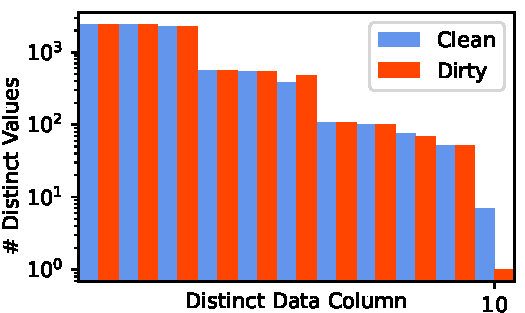
\includegraphics[width=\textwidth]{figures/plot/distinct/beers_distinct/combined.pdf}
    \caption{\label{exp:d1}Bears}
    \label{exp:distincts_bears}
\end{subfigure}
\hfill
\begin{subfigure}{0.4\textwidth}
    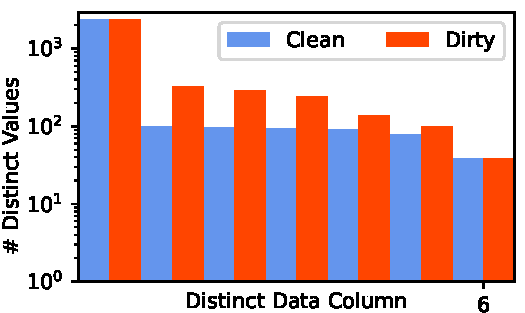
\includegraphics[width=\textwidth]{figures/plot/distinct/flights_distinct/combined.pdf}
    \caption{Flights}
    \label{exp:distincts_flights}
\end{subfigure}
\hfill
\begin{subfigure}{0.4\textwidth}
    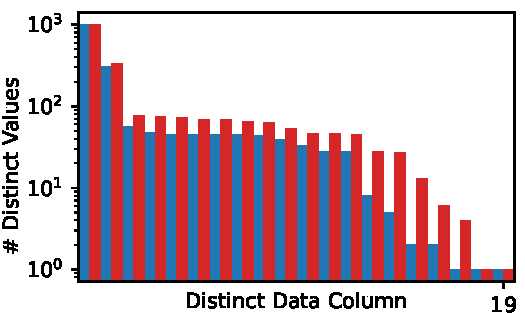
\includegraphics[width=\textwidth]{figures/plot/distinct/hospital_distinct/combined.pdf}
    \caption{Hospital}
    \label{fig:distincts_hospitals}
\end{subfigure}
\hfill
\begin{subfigure}{0.4\textwidth}
    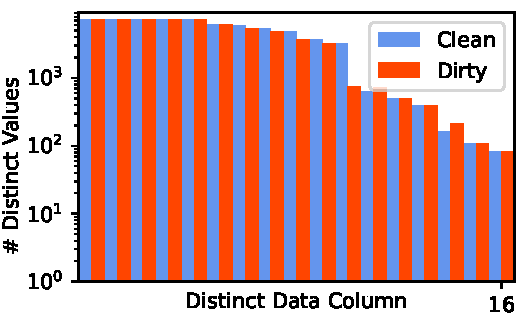
\includegraphics[width=\textwidth]{figures/plot/distinct/movies_distinct/combined.pdf}
    \caption{Movies}
    \label{exp:distincts_movies}
\end{subfigure}
\hfill
\begin{subfigure}{0.4\textwidth}
    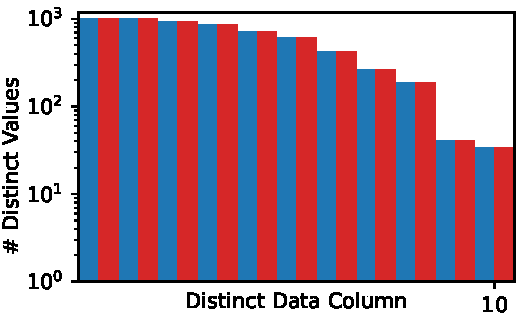
\includegraphics[width=\textwidth]{figures/plot/distinct/rayyan_distinct/combined.pdf}
    \caption{Rayyan}
    \label{exp:distincts_rayyan}
\end{subfigure}
\hfill
\begin{subfigure}{0.4\textwidth}
    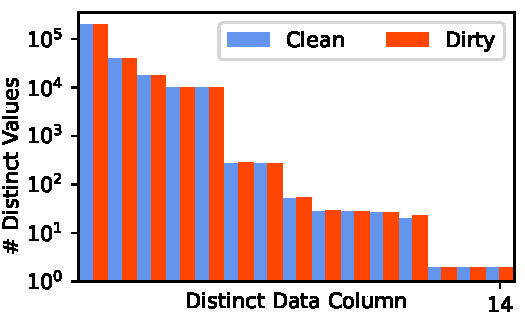
\includegraphics[width=\textwidth]{figures/plot/distinct/tax_distinct/combined.pdf}
    \caption{Tax}
    \label{exp:distincts_tax}
\end{subfigure}
\hfill
% TODO describe 
        
\caption{Distinct values distribution of clean and dirty datasets}
\label{exp:distinct_values_datasets}
\end{figure}
Figure \ref{exp:distinct_values_datasets} shows the number of distinct values and their frequencies in each dataset. 

\subsection{Error distribution}
To preserve the error distribution in generated dataset, error characteristics of the original dirty are %TODO.
\begin{table}[!t]
\caption{\label{tab:dirty_num_errors}Dirty dataset error characteristics}
\begin{tabular}{r|l|l|l|l|l}
\toprule
                     & Outliers & Typos & Missing values & Replacement & Swaps \\ \midrule
beers                & 0        & 254   & 4170           & 0                & 0       \\
flights              & 0        & 2243  & 0              & 0                & 314     \\
hospital             & 0        & 417   & 92             & 0                & 0       \\
movies               & 0        & 982   & 6346           & 141              & 0       \\
rayyan               & 0        & 649   & 75             & 224              & 0       \\
tax                  & 2        & 1367  & 588            & 1200             & 4       \\ \bottomrule
\end{tabular}
\end{table}
% TODO Replacement vs Flipped category vs Flipped value
In Table \ref{tab:dirty_num_errors} number of errors in every dataset.

% TODO Each column which type of error is present in which column.
\begin{figure}[!t]
    \centering 
    \centering
\begin{subfigure}{0.4\textwidth}
    \includegraphics[width=\textwidth]{example-image-a}
    \caption{\label{exp:d1}Bears}
    \label{exp:barplot_error_count_bears}
\end{subfigure}
\hfill
\begin{subfigure}{0.4\textwidth}
    \includegraphics[width=\textwidth]{example-image-a}
    \caption{Flights}
    \label{exp:barplot_error_count_flights}
\end{subfigure}
\hfill
\begin{subfigure}{0.4\textwidth}
    \includegraphics[width=\textwidth]{example-image-a}
    \caption{Hospital}
    \label{fig:barplot_error_count_hospital}
\end{subfigure}
\hfill
\begin{subfigure}{0.4\textwidth}
    \includegraphics[width=\textwidth]{example-image-a}
    \caption{Movies}
    \label{exp:barplot_error_count_movies}
\end{subfigure}
\hfill
\begin{subfigure}{0.4\textwidth}
    \includegraphics[width=\textwidth]{example-image-a}
    \caption{Rayyan}
    \label{exp:barplot_error_count_rayyan}
\end{subfigure}
\hfill
\begin{subfigure}{0.4\textwidth}
    \includegraphics[width=\textwidth]{example-image-a}
    \caption{Tax}
    \label{exp:distincts_tax}
\end{subfigure}
\hfill
\begin{subfigure}{0.4\textwidth}
    \includegraphics[width=\textwidth]{example-image-a}
    \caption{Toy}
    \label{exp:barplot_error_count_toy}
\end{subfigure}
\caption{Number of errors in each dataset}
\label{exp:barplot_error_counts_datasets}
\end{figure}
\section{Scaling up}

Experiments with different scaling up. How close statistics are to actual?
Table with stats before after for each method
copy + random
copy + slice
fully random



\section{Runtime experiments}
Runtime experiments with how long it takes local & distributed. 
Stacked bar charts (size vs time) for different data sizes. 
Expected to be linear (10 TB ?! measure by hours).
\chapter{Conclusions}
% What follows
The framework proposed in this work initiates the large-scale generation of dirty data, in which original real-world observations are used to extract error patterns and create new observations.
The new data generation framework scales existing datasets while preserving error distribution and statistics.
The experiments show linear performance in distributed execution, and super linear in local execution.
The biggest data size generated is 18 GB that corresponds to a scaling factor of 65536x.
Six different datasets with ground truth were used for experiments: five real-world and one synthetic.
Different scaling factors were tested on all datasets.
Thus, it is demonstrated that it is possible to generate large datasets while preserving statistics of a small sample of dirty data.

% Lessons Learned
It is challenging to generate datasets with statistical properties of the original dirty dataset.
In this context, execution and optimization of distributed workloads is a non-trivial and time-consuming task.
Researching the context of data cleaning and studying existing state-of-the-art frameworks also brought many insights of what can be done and improved.
But the faced challenges were handled, and turned into the improvements of the framework and lessons learned.

% Limitations and Future Work - 3 paragraphs
Interesting directions for future work include 
(1) understanding of existing skew of Spark tasks and optimization of the distributed execution
(2) optimization of the local execution, 
(3) more advanced and fine-grained error detection and classification algorithms,
(4) support of more error types, 
(5) integration into data cleaning benchmarks, and
(6) different techniques for scaling up such as random.
 

% % Say what your solution achieves (200 words)
% Hence, this work focuses on data generation, observations of the original clean and dirty data are used to scale up to arbitrary data sizes.
% The biggest scaling factor achieved is 65536x, and the largest data size achieved was 18 GB.
% These results were gained under the constraints of preserving data statistics and error distribution, and, therefore, new algorithms were applied.
% The generator can run either locally, or distributed via Apache Spark.
% As expected, the local execution is faster for small scaling factors up to 42x, 
% while, on the other hand, when scaling to larger sizes the distributed execution performs better.
% % Say what follows from your solution (25 words)
% Starting out, it was challenging to introduce errors preserving characteristics of the original dataset. 
% % since such errors as e.g. outliers change the mean drastically.
% The proposed framework solves the large-scale data generation problem, and provides a solution for cleaning for ML benchmarks by scaling data and its distribution.



\setmaxbibnames{999}
\printbibliography              %% remove, if using BibTeX instead of biblatex
% \include{further_ressources}  %% this is a suggestion: you have to create this file on demand

\appendix


% \chapter{Error counts scaling}
% \label{apendix:error_counts_scaling}

% Error counts for the different datasets:

% \begin{table}[!ht]
% \caption{\label{tab:local_errors_beers} Local error distribution in beers}
% \centering
% \begin{tabular}{r|K|K|K|K|K}
% \toprule
% \colCenter{Scale} & \colCenter{Outliers} & \colCenter{Typos} & \colCenter{MV} & \colCenter{Rep} & \colCenterNoRight{Swaps} \\ \midrule
% \numprint{1}    & \numprint{0}        & \numprint{254}          & \numprint{4170}                 &  \numprint{0}     &  \numprint{0}              \\
% \numprint{2}    & \numprint{0}        & \numprint{508}          & \numprint{8340}                 &  \numprint{0}     &  \numprint{0}              \\
% \numprint{4}    & \numprint{0}        & \numprint{101}          & \numprint{16680}                 &  \numprint{0}     &  \numprint{0}              \\
% \numprint{8}    & \numprint{0}        & \numprint{203}          & \numprint{33360}                 &  \numprint{0}     &  \numprint{0}              \\
% \numprint{16}   & \numprint{0}        & \numprint{406}          & \numprint{66720}                 &  \numprint{0}     &  \numprint{0}              \\
% \numprint{32}   & \numprint{0}        & \numprint{812}          & \numprint{133440}                 &  \numprint{0}     &  \numprint{0}              \\
% \numprint{64}   & \numprint{0}        & \numprint{162}          & \numprint{266880}                 &  \numprint{0}     &  \numprint{0}              \\
% \numprint{128}  & \numprint{0}        & \numprint{325}          & \numprint{533760}                 &  \numprint{0}     &  \numprint{0}              \\
% \numprint{256}  & \numprint{0}        & \numprint{650}          & \numprint{1067520}                 &  \numprint{0}     &  \numprint{0}              \\
% \bottomrule
% \end{tabular}
% \end{table}

% \begin{table}[!ht]
% \caption{\label{tab:local_errors_flights} Local error distribution in flights}
% \centering
% \begin{tabular}{r|K|K|K|K|K}
% \toprule
% \colCenter{Scale} & \colCenter{Outliers} & \colCenter{Typos} & \colCenter{MV} & \colCenter{Rep} & \colCenterNoRight{Swaps}  \\ \midrule
% \numprint{1}             & \numprint{0}        & \numprint{4606}    & \numprint{0}             &  \numprint{314}  &  \numprint{0}              \\
% \numprint{2}             & \numprint{0}        & \numprint{9212}    & \numprint{0}             &  \numprint{628}  &  \numprint{0}              \\
% \numprint{4}             & \numprint{0}        & \numprint{18424}          & \numprint{0}             &  \numprint{1256}     &  \numprint{0}              \\
% \numprint{8}             & \numprint{0}        & \numprint{36848}          & \numprint{0}             &  \numprint{2512}     &  \numprint{0}              \\
% \numprint{16}             & \numprint{0}        & \numprint{73696}          & \numprint{0}             &  \numprint{5024}     &  \numprint{0}              \\
% \numprint{32}             & \numprint{0}        & \numprint{147392}          & \numprint{0}             &  \numprint{10048}     &  \numprint{0}              \\
% \numprint{64}             & \numprint{0}        & \numprint{294784}          & \numprint{0}             &  \numprint{20096}     &  \numprint{0}              \\
% \numprint{128} & \numprint{0} & \numprint{589568}  & \numprint{0} & \numprint{40192} & \numprint{0} \\
% \numprint{256} & \numprint{0} & \numprint{1179136} & \numprint{0} & \numprint{80384} & \numprint{0} \\
% \bottomrule
% \end{tabular}
% \end{table}

% \begin{table}[!ht]
% \caption{\label{tab:local_errors_hospital} Local error distribution in hospital}
% \centering
% \begin{tabular}{r|K|K|K|K|K}
% \toprule
% \colCenter{Scale} & \colCenter{Outliers} & \colCenter{Typos} & \colCenter{MV} & \colCenter{Rep} & \colCenterNoRight{Swaps}  \\ \midrule
% \numprint{1}        & \numprint{0}        & \numprint{417}         & \numprint{92}                &  \numprint{0}       &  \numprint{0}     \\
% \numprint{2}        & \numprint{0}        & \numprint{834}         & \numprint{184}               &  \numprint{0}       &  \numprint{0}     \\
% \numprint{4}        & \numprint{0}        & \numprint{1668}        & \numprint{368}               &  \numprint{0}       &  \numprint{0}     \\
% \numprint{8}        & \numprint{0}        & \numprint{3336}        & \numprint{736}               &  \numprint{0}       &  \numprint{0}     \\
% \numprint{16}       & \numprint{0}        & \numprint{6672}        & \numprint{1472}              &  \numprint{0}       &  \numprint{0}     \\
% \numprint{32}       & \numprint{0}        & \numprint{13344}       & \numprint{2944}              &  \numprint{0}       &  \numprint{0}     \\
% \numprint{64}       & \numprint{0}        & \numprint{26688}       & \numprint{5888}              &  \numprint{0}       &  \numprint{0}     \\ 
% \numprint{128}      & \numprint{0}        & \numprint{53376}       & \numprint{11776}             &  \numprint{0}       &  \numprint{0}     \\
% \numprint{256}      & \numprint{0}        & \numprint{106752}      & \numprint{23552}             &  \numprint{0}       &  \numprint{0}     \\
% \bottomrule
% \end{tabular}
% \end{table}

% \begin{table}[!ht]
% \caption{\label{tab:local_errors_movies} Local error distribution in movies}
% \centering
% \begin{tabular}{r|K|K|K|K|K}
% \toprule
% \colCenter{Scale} & \colCenter{Outliers} & \colCenter{Typos} & \colCenter{MV} & \colCenter{Rep} & \colCenterNoRight{Swaps}  \\ \midrule
% \numprint{1}        & \numprint{0}        & \numprint{982}      & \numprint{6346}       &  \numprint{142}   &  \numprint{0}       \\
% \numprint{2}        & \numprint{0}        & \numprint{1964}     & \numprint{12692}      &  \numprint{284}   &  \numprint{0}       \\
% \numprint{4}        & \numprint{0}        & \numprint{3928}     & \numprint{25384}      &  \numprint{568}   &  \numprint{0}       \\
% \numprint{8}        & \numprint{0}        & \numprint{7856}     & \numprint{50768}      &  \numprint{1136}  &  \numprint{0}       \\
% \numprint{16}       & \numprint{0}        & \numprint{15712}    & \numprint{101536}     &  \numprint{2272}  &  \numprint{0}       \\
% \numprint{32}       & \numprint{0}        & \numprint{31424}    & \numprint{203072}     &  \numprint{4544}  &  \numprint{0}       \\
% \numprint{64}       & \numprint{0}        & \numprint{62848}    & \numprint{406144}     &  \numprint{9088}  &  \numprint{0}       \\
% \numprint{128}      & \numprint{0}        & \numprint{125696}   & \numprint{812288}     &  \numprint{18176} &  \numprint{0}       \\ 
% \numprint{256}      & \numprint{0}        & \numprint{251392}   & \numprint{1624576}    &  \numprint{36352} &  \numprint{0}       \\   \bottomrule
% \end{tabular}
% \end{table}

% \begin{table}[!ht]
% \caption{\label{tab:local_errors_rayyan} Local error distribution in rayyan}
% \centering
% \begin{tabular}{r|K|K|K|K|K}
% \toprule
% \colCenter{Scale} & \colCenter{Outliers} & \colCenter{Typos} & \colCenter{MV} & \colCenter{Rep} & \colCenterNoRight{Swaps}  \\ \midrule
% \numprint{1}         & \numprint{0}        & \numprint{649}       & \numprint{75}       &  \numprint{224}       &  \numprint{0}              \\
% \numprint{2}         & \numprint{0}        & \numprint{1298}      & \numprint{150}      &  \numprint{448}       &  \numprint{0}              \\
% \numprint{4}         & \numprint{0}        & \numprint{2596}      & \numprint{300}      &  \numprint{896}       &  \numprint{0}              \\
% \numprint{8}         & \numprint{0}        & \numprint{5192}      & \numprint{600}      &  \numprint{1792}      &  \numprint{0}              \\
% \numprint{16}        & \numprint{0}        & \numprint{10384}     & \numprint{1200}     &  \numprint{3584}      &  \numprint{0}              \\
% \numprint{32}        & \numprint{0}        & \numprint{20768}     & \numprint{2400}     &  \numprint{7168}      &  \numprint{0}              \\
% \numprint{64}        & \numprint{0}        & \numprint{41536}     & \numprint{4800}     &  \numprint{14336}     &  \numprint{0}              \\ 
% \numprint{128}       & \numprint{0}        & \numprint{83072}     & \numprint{9600}     &  \numprint{28672}     &  \numprint{0}              \\ 
% \numprint{256}       & \numprint{0}        & \numprint{166144}    & \numprint{19200}    &  \numprint{57344}     &  \numprint{0}              \\  \bottomrule
% \end{tabular}
% \end{table}

\newpage
\chapter{Distinct Errors Scaling}
\label{apendix:distinct_errors_scaling}

Scaling the distinct errors for the different datasets.

% \begin{table}[!ht]
% \caption{\label{tab:dist_errors_beer} Local errors distincts in beer}
% \centering
% \begin{tabular}{r|H|H|H|H|H|H}
%               & \multicolumn{2}{c|}{\textbf{Typos}}   & \multicolumn{2}{c|}{\textbf{MV}}  & \multicolumn{2}{c}{\textbf{Distinct}}\\
% \colCenter{Scale} & \colCenter{Est} & \colCenter{Act} & \colCenter{Est} & \colCenter{Act} & \colCenter{Est}   & \colCenterNoRight{Act}   \\ \midrule
% \numprint{1}          &  \numprint{97}      & \numprint{97}          & \numprint{3}  & \numprint{6}  & \numprint{9038}  & \numprint{9038}     \\
% \numprint{2}          &  \numprint{167}     & \numprint{167}         & \numprint{3}  & \numprint{6}  & \numprint{9128}  & \numprint{9116}     \\
% \numprint{4}          &  \numprint{290}     & \numprint{290}         & \numprint{3}  & \numprint{6}  & \numprint{9251}  & \numprint{9241}     \\
% \numprint{8}          &  \numprint{526}     & \numprint{526}         & \numprint{3}  & \numprint{6}  & \numprint{9487}  & \numprint{9474}     \\
% \numprint{16}         &  \numprint{994}     & \numprint{994}         & \numprint{3}  & \numprint{6}  & \numprint{9955}  & \numprint{9938}     \\
% \numprint{32}         &  \numprint{1926}    & \numprint{1923}        & \numprint{3}  & \numprint{6}  & \numprint{10887}  & \numprint{10866}     \\
% \numprint{64}         &  \numprint{3789}    & \numprint{3786}        & \numprint{3}  & \numprint{6}  & \numprint{12750}  & \numprint{12699}     \\ 
% \numprint{128}        &  \numprint{7514}    & \numprint{7405}        & \numprint{3}  & \numprint{6}  & \numprint{16475}  & \numprint{16290}     \\
% \numprint{256}        &  \numprint{14964}   & \numprint{14575}       & \numprint{3}  & \numprint{6}  & \numprint{23925}  & \numprint{23420}     \\
% \bottomrule
% \end{tabular}
% \end{table}

% \begin{table}[!ht]
% \caption{\label{tab:dist_errors_flights} Local errors distincts in flights}
% \centering
% \begin{tabular}{r|H|H|H|H|H|H}
%               & \multicolumn{2}{c|}{\textbf{Typos}}   & \multicolumn{2}{c|}{\textbf{MV}}  & \multicolumn{2}{c}{\textbf{Distinct}}\\
% \colCenter{Scale} & \colCenter{Est} & \colCenter{Act} & \colCenter{Est} & \colCenter{Act} & \colCenter{Est}   & \colCenterNoRight{Act}   \\ \midrule
% \numprint{1}         & \numprint{651}   & \numprint{651}    & \numprint{0}  & \numprint{0}  & \numprint{3512}   & \numprint{3512}    \\
% \numprint{2}         & \numprint{808}   & \numprint{808}    & \numprint{0}  & \numprint{0}  & \numprint{3682}   & \numprint{3682}    \\
% \numprint{4}         & \numprint{1012}  & \numprint{1012}   & \numprint{0}  & \numprint{0}  & \numprint{3886}   & \numprint{3883}    \\
% \numprint{8}         & \numprint{1334}  & \numprint{1334}   & \numprint{0}  & \numprint{0}  & \numprint{4208}   & \numprint{4204}    \\
% \numprint{16}        & \numprint{1940}  & \numprint{1937}   & \numprint{0}  & \numprint{0}  & \numprint{4814}   & \numprint{4796}    \\
% \numprint{32}        & \numprint{3136}  & \numprint{3126}   & \numprint{0}  & \numprint{0}  & \numprint{6010}   & \numprint{5974}    \\
% \numprint{64}        & \numprint{5521}  & \numprint{5473}   & \numprint{0}  & \numprint{0}  & \numprint{8395}   & \numprint{8309}    \\
% \numprint{128}       & \numprint{10151} & \numprint{10012}  & \numprint{0}  & \numprint{0}  & \numprint{13025}  & \numprint{12816}     \\
% \numprint{256}       & \numprint{17301} & \numprint{16968}  & \numprint{0}  & \numprint{0}  & \numprint{20175}  & \numprint{19728}     \\
% \bottomrule
% \end{tabular}
% \end{table}

% \begin{table}[!ht]
% \caption{\label{tab:dist_errors_hospital} Local errors distincts in hospital}
% \centering
% \begin{tabular}{r|H|H|H|H|H|H}
%               & \multicolumn{2}{c|}{\textbf{Typos}}   & \multicolumn{2}{c|}{\textbf{MV}}  & \multicolumn{2}{c}{\textbf{Distinct}}\\
% \colCenter{Scale} & \colCenter{Est} & \colCenter{Act} & \colCenter{Est} & \colCenter{Act} & \colCenter{Est}   & \colCenterNoRight{Act}   \\ \midrule
% \numprint{1}         & \numprint{311}   & \numprint{311}  & \numprint{3}  & \numprint{3}  & \numprint{2094} & \numprint{2094}    \\
% \numprint{2}         & \numprint{568}   & \numprint{568}  & \numprint{3}  & \numprint{6}  & \numprint{2357} & \numprint{2355}    \\
% \numprint{4}         & \numprint{1060}  & \numprint{1058}  & \numprint{3}  & \numprint{6}  & \numprint{2849} & \numprint{2841}    \\
% \numprint{8}         & \numprint{2039}  & \numprint{2037}  & \numprint{3}  & \numprint{6}  & \numprint{3828} & \numprint{3809}    \\
% \numprint{16}        & \numprint{3992}  & \numprint{3977}  & \numprint{3}  & \numprint{6}  & \numprint{5781} & \numprint{5735}    \\
% \numprint{32}        & \numprint{7899}  & \numprint{7839}  & \numprint{3}  & \numprint{6}  & \numprint{9688} & \numprint{9571}    \\
% \numprint{64}        & \numprint{15711} & \numprint{15493}  & \numprint{3}  & \numprint{6}  & \numprint{17200} & \numprint{17181}     \\ 
% \numprint{128}       & \numprint{31336} & \numprint{30223}  & \numprint{3}  & \numprint{6}  & \numprint{33125} & \numprint{31801}     \\ 
% \numprint{256}       & \numprint{62584} & \numprint{59268}  & \numprint{3}  & \numprint{6}  & \numprint{64373} & \numprint{60722}     \\ 
% \bottomrule
% \end{tabular}
% \end{table}

% \begin{table}[!ht]
% \caption{\label{tab:dist_errors_movies} Local errors distincts in movies}
% \centering
% \begin{tabular}{r|H|H|H|H|K|K}
%               & \multicolumn{2}{c|}{\textbf{Typos}}   & \multicolumn{2}{c|}{\textbf{MV}}  & \multicolumn{2}{c}{\textbf{Distinct}}\\
% \colCenter{Scale} & \colCenter{Est} & \colCenter{Act} & \colCenter{Est} & \colCenter{Act} & \colCenter{Est}   & \colCenterNoRight{Act}   \\ \midrule
% \numprint{1}        & \numprint{868}    & \numprint{868}    & \numprint{3}  & \numprint{3}  & \numprint{62444}  & \numprint{62444}    \\
% \numprint{2}        & \numprint{1667}   & \numprint{1667}   & \numprint{3}  & \numprint{6}  & \numprint{69010}  & \numprint{68659}    \\
% \numprint{4}        & \numprint{3227}   & \numprint{3226}   & \numprint{3}  & \numprint{6}  & \numprint{70570}  & \numprint{68547}    \\
% \numprint{8}        & \numprint{6321}   & \numprint{6317}   & \numprint{3}  & \numprint{6}  & \numprint{73664}  & \numprint{72970}    \\
% \numprint{16}       & \numprint{12498}  & \numprint{12494}  & \numprint{3}  & \numprint{6}  & \numprint{79841}  & \numprint{79702}    \\
% \numprint{32}       & \numprint{24846}  & \numprint{24833}  & \numprint{3}  & \numprint{6}  & \numprint{92189}  & \numprint{92066}    \\
% \numprint{64}       & \numprint{49539}  & \numprint{49486}  & \numprint{3}  & \numprint{6}  & \numprint{116882} & \numprint{116613}     \\ 
% \numprint{128}      & \numprint{98924}  & \numprint{98746}  & \numprint{3}  & \numprint{6}  & \numprint{166267} & \numprint{165632}     \\ 
% \numprint{256}      & \numprint{197695} & \numprint{197100} & \numprint{3}  & \numprint{6}  & \numprint{265038} & \numprint{263634}     \\ 

% \bottomrule
% \end{tabular}
% \end{table}


\chapter{Local Min Max scaled difference}
\label{apendix:min_max_local_difference}

% The differences in percent but for min and max

% \begin{figure}[!ht]
%     \centering 
%     \centering
% \begin{subfigure}{0.32\textwidth}
%     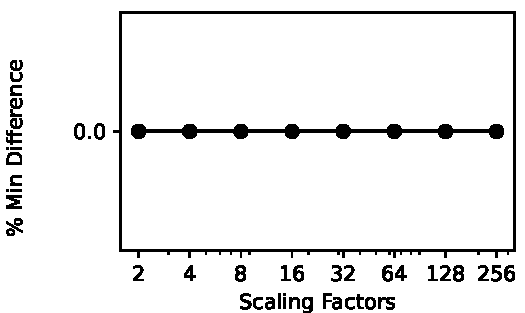
\includegraphics[width=\textwidth]{figures/plot/min/min_diff_beers.pdf}
%     \caption{Bears}
%     \label{exp:min_bears}
% \end{subfigure}
% \hfill
% \begin{subfigure}{0.32\textwidth}
%     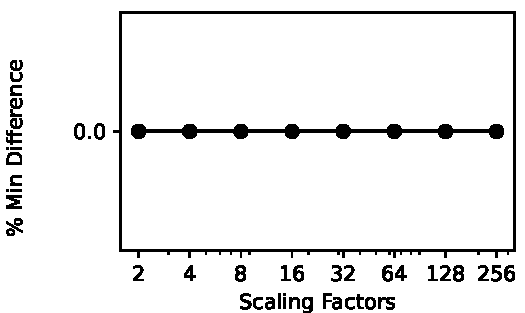
\includegraphics[width=\textwidth]{figures/plot/min/min_diff_flights.pdf}
%     \caption{Flights}
%     \label{exp:min_flights}
% \end{subfigure}
% \hfill
% \begin{subfigure}{0.32\textwidth}
%     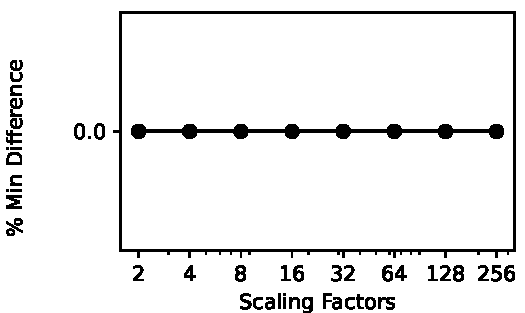
\includegraphics[width=\textwidth]{figures/plot/min/min_diff_hospital.pdf}
%     \caption{Hospital}
%     \label{fig:min_hospitals}
% \end{subfigure}
% \hfill
% \begin{subfigure}{0.32\textwidth}
%     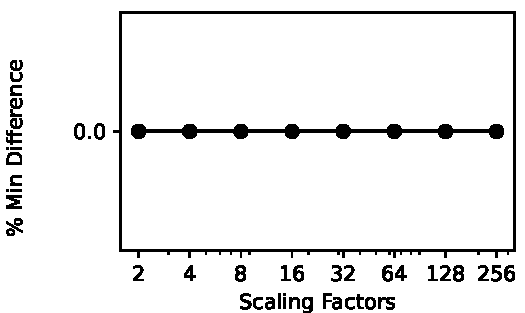
\includegraphics[width=\textwidth]{figures/plot/min/min_diff_movies.pdf}
%     \caption{Movies}
%     \label{exp:min_movies}
% \end{subfigure}
% \hfill
% \begin{subfigure}{0.32\textwidth}
%     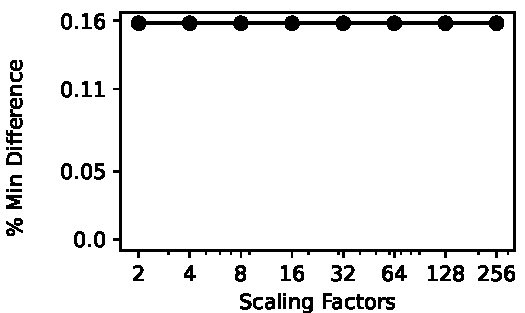
\includegraphics[width=\textwidth]{figures/plot/min/min_diff_rayyan.pdf}
%     \caption{Rayyan}
%     \label{exp:min_rayyan}
% \end{subfigure}
% \hfill
% \begin{subfigure}{0.32\textwidth}
%     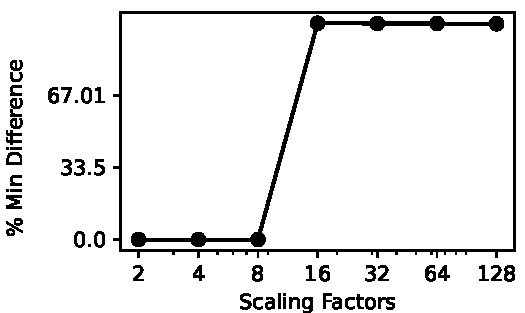
\includegraphics[width=\textwidth]{figures/plot/min/min_diff_tax.pdf}
%     \caption{Tax}
%     \label{exp:min_tax}
% \end{subfigure}
% \hfill
% \caption{Min value difference in percent scaling clean and dirty datasets}
% \label{exp:min_difference_datasets}
% \end{figure}



% \begin{figure}[!ht]
%     \centering 
%     \centering
% \begin{subfigure}{0.32\textwidth}
%     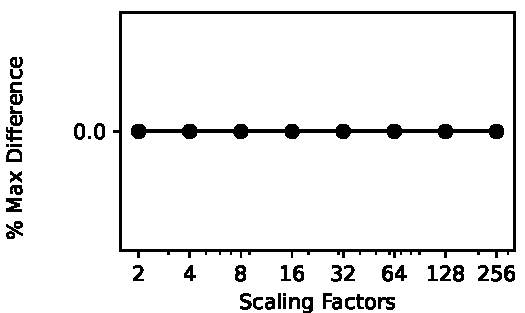
\includegraphics[width=\textwidth]{figures/plot/max/max_diff_beers.pdf}
%     \caption{Bears}
%     \label{exp:max_bears}
% \end{subfigure}
% \hfill
% \begin{subfigure}{0.32\textwidth}
%     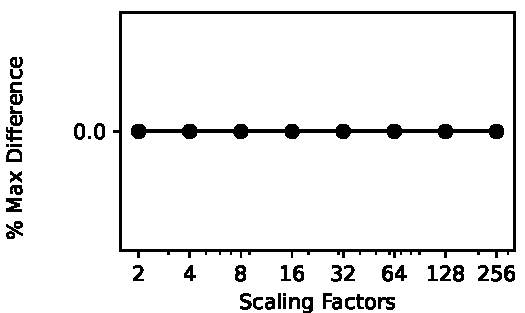
\includegraphics[width=\textwidth]{figures/plot/max/max_diff_flights.pdf}
%     \caption{Flights}
%     \label{exp:max_flights}
% \end{subfigure}
% \hfill
% \begin{subfigure}{0.32\textwidth}
%     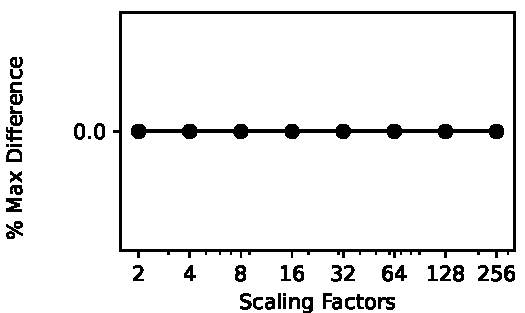
\includegraphics[width=\textwidth]{figures/plot/max/max_diff_hospital.pdf}
%     \caption{Hospital}
%     \label{fig:max_hospitals}
% \end{subfigure}
% \hfill
% \begin{subfigure}{0.32\textwidth}
%     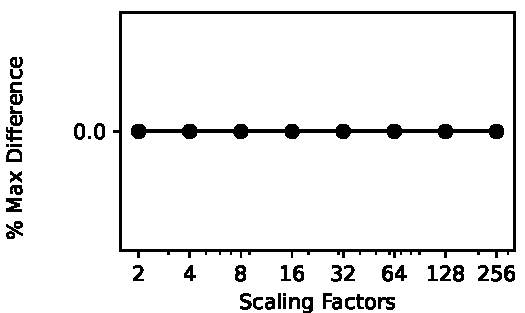
\includegraphics[width=\textwidth]{figures/plot/max/max_diff_movies.pdf}
%     \caption{Movies}
%     \label{exp:max_movies}
% \end{subfigure}
% \hfill
% \begin{subfigure}{0.32\textwidth}
%     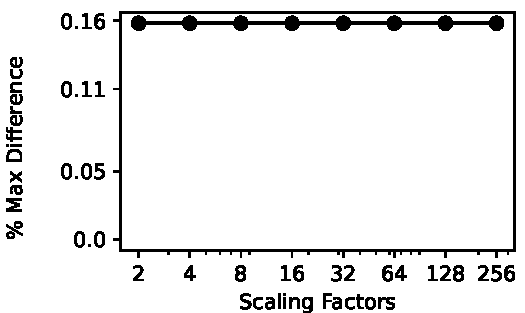
\includegraphics[width=\textwidth]{figures/plot/max/max_diff_rayyan.pdf}
%     \caption{Rayyan}
%     \label{exp:max_rayyan}
% \end{subfigure}
% \hfill
% \begin{subfigure}{0.32\textwidth}
%     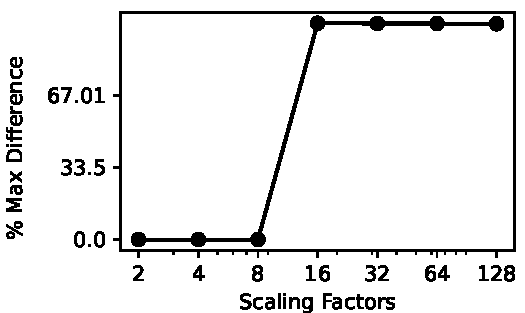
\includegraphics[width=\textwidth]{figures/plot/max/max_diff_tax.pdf}
%     \caption{Tax}
%     \label{exp:max_tax}
% \end{subfigure}
% \hfill
% \caption{Max value difference in percent scaling clean and dirty datasets}
% \label{exp:max_difference_datasets}
% \end{figure}





%%%% end{document}
\end{document}
%% vim:foldmethod=expr
%% vim:fde=getline(v\:lnum)=~'^%%%%\ .\\+'?'>1'\:'='
%%% Local Variables:
%%% mode: latex
%%% mode: auto-fill
%%% mode: flyspell
%%% eval: (ispell-change-dictionary "en_US")
%%% TeX--: "main"
%%% End:
